\documentclass[plainarticle,zihtitle,english,final,hyperref,utf8]{zihpub}
\usepackage[toc,page]{appendix}
\usepackage{setspace}
\usepackage{fancyvrb}
\usepackage{fvextra}
\usepackage{hyperref}
\usepackage{multirow}
\usepackage[table,xcdraw]{xcolor}
\hypersetup{
    colorlinks=true,
    linkcolor=blue,
    filecolor=magenta,      
    urlcolor=cyan,
}
\usepackage{multirow}
\usepackage{graphicx}
\usepackage{csquotes}
\renewcommand{\mkbegdispquote}[2]{\itshape}

\author{Oliver Braun - Eszter Schuffert - Marine Elise Lafin}
\title{\textbf{Possible Use Cases for TurtleBot3 and OpenManipulator-X and its simulation} \\ \bigskip Documentation}
\bibfiles{doku}
\betreuer{David Gollasch}


\begin{document}
\listoftables
\listoffigures
\newpage

\section{Introduction}
The TurtleBot3 and the OpenManipulator-X have recently been acquired by the Chair of Human-Computer-Interaction at the TU Dresden for educational purposes.\\
\newline
It was first of interest to have a look at the possible use case scenarios of this robot to assist various groups of people with certain disabilities, such as a reduced range of motion or blindness. These are based upon the theoretical functionalities and specifications of the TurtleBot3 and the OpenManipulator Arm, as well as observed capabilities. Those use cases should be able to be implemented within small group projects and all are thought to support people within a care context.\\
\newline
The main motivation and inspiration behind the use cases is the job of one of the authors of this paper at the Dresden Uniklinikum hospital, in services with a heavy influx of elderly patients which is an area where a support robot could be helpful (section \ref{sec:appendix}). Therefore, to further access whether the nursing staff would see some of the formulated Use Cases as helpful, a small survey was carried out to analyse whether first of all the TurtleBot3 in itself was seen as suitable by the staff to carry out any tasks in a care environment.
Then, it was researched whether the the three Use Cases were relevant to the chosen demographic - elderly people who are in need of care and support.
Furthermore, the last information which was important, is the personal assessment as to whether or not such a robot would be accepted by the population. This might be a subjective sentiment but will help guide the paper in the right direction to design Use Cases which have a higher probability to be accepted by the wider public.\\
\newline
In this paper, three personas were designed to further aid the description of the proposed Use Cases for TurtleBot3. Their main areas disabilities are visual impairment and mobility issues, furthermore two of the personas are elderly people which suffer from some level of solitude and isolation. The third persona is a working nurse which was based upon a single person known to the authors.\\
\newline
Through those personas, three Use Cases will be explored; the paper will look at the possibility of the TurtleBot distributing/transporting medicine to patients, socialise with its owner through listening to their stories with further functionalities and guiding a person through a known area equipped with beacons.\\
\newline
One limitation of those proposed use cases is that, none could be further studied in relation to the perceived benefit by the group of people whom the robot would assist. The Use Cases should be therefore regarded as theoretical cases which could be implemented within the constraint of a research project. Further research would have to be pursued in order to access the feasibility and benefits of these various use cases.\\
\newline
A further limitation would be that some of the use cases are based upon hardware, such as various sensors, not present at the TU Dresden. Therefore, their limitations could not be assessed accurately. This could possible lead to a malfunctioning robot if the use cases where to be implemented.\\
\newline
Due to the strict confinement and social distancing rules put in place by governments worldwide to slow down the spread of the COVID-19 virus in the Summer semester 2020, the idea to examine the functionalities of the robot and its arm (OpenManipulator) remotely became a focus point. Therefore, several avenues had to be explored to simulate this robot, to be able test possible future programs without physical access to the robot while maintaining successful collaboration between team members.\\
\newline
Based upon the documentation of the TurtleBot3 and its arm \cite{tb3docu} \cite{openmandocu}, attempts were made at simulating it in various ways using the Gazebo simulation software recommended by the TurtleBot developers. It was quickly discovered that the available documentation was either incomplete or inaccurate, and therefore a more exhaustive guide would be of good use for future programmers wishing to simulate the robot. Therefore, a step by step guide will be provided, as well as a complimentary comment as to how to avoid certain known problems or possible encountered dead-ends.\\
\newline
Each simulation environment which was attempted had a clear list of advantages and drawbacks which will be further discussed in this paper to further aid the decision as to which simulation environment to use for the best result. The main focus will be put on the following simulation environments: the standalone installation of Ubuntu with either ROS1 or ROS2, the installation of Ubuntu within the constraints of a Virtual Machine as well as two cloud solutions: AWS (Amazon) and the Gazebo Web client.\\
\newline
Some more possibilities will be presented and links to further literature will be provided to aid any future user in finding a simulation environment for TurtleBot3 and its arm, which fits their needs.\\
\newline
The scope of the paper is limited by the technical difficulties faced during different setups as well as a lack of resources, may it be due to lack of hardware or financial funds. Furthermore, this paper can only assess available possible software versions up until August 2020.\\
\newpage
\section{Capabilities of the Turtlebot}
This chapter focuses on hardware specifications of the TurtleBot3 \textit{waffle\_pi} model and the OpenManipulator-X arm and our own experiences setting up and working with the robot in the lab. First a general overview of selected specifications is listed in table \ref{tab:specifications}. The following links will provide additional information about the \href{https://emanual.robotis.com/docs/en/platform/turtlebot3/specifications/#specifications}{TurtleBot3} and \href{https://emanual.robotis.com/docs/en/platform/openmanipulator_x/specification/#specification}{OpenManipulator-X} specifications.\\
\newline
Understanding the capabilities of a robot is hard without physical contact. Therefore we organized scheduled meetings with the TurtleBot3 to test the set up instructions and get an overall impression of the robot. The instructions for the setup can be found \href{https://emanual.robotis.com/docs/en/platform/turtlebot3/setup/#setup}{here}. Going through the PC Setup and SBC Setup guaranteed us a stable connection between a Remote PC and the TurtleBot's Raspberry Pi. Thankfully, the Hardware Setup was not necessary anymore, because it was already assembled. For future uses it might be advised to reposition interfaces (https://ubuntu.com/blog/building-a-better-turtlebot3), so the Raspberry Pi is more accessible from outside in order to better reach components such as the microSD card slot. Before control could be established the Bringup section of the TurtleBot3 documentation had to be applied. Here we got following error as seen in figure \ref{fig:errorbringup}, which points to connectivity issues. There are some possible solutions if the error output is searched. However, we did not manage to fix them as there were time constraints.\\
\begin{figure}[h!]
  \begin{center}
    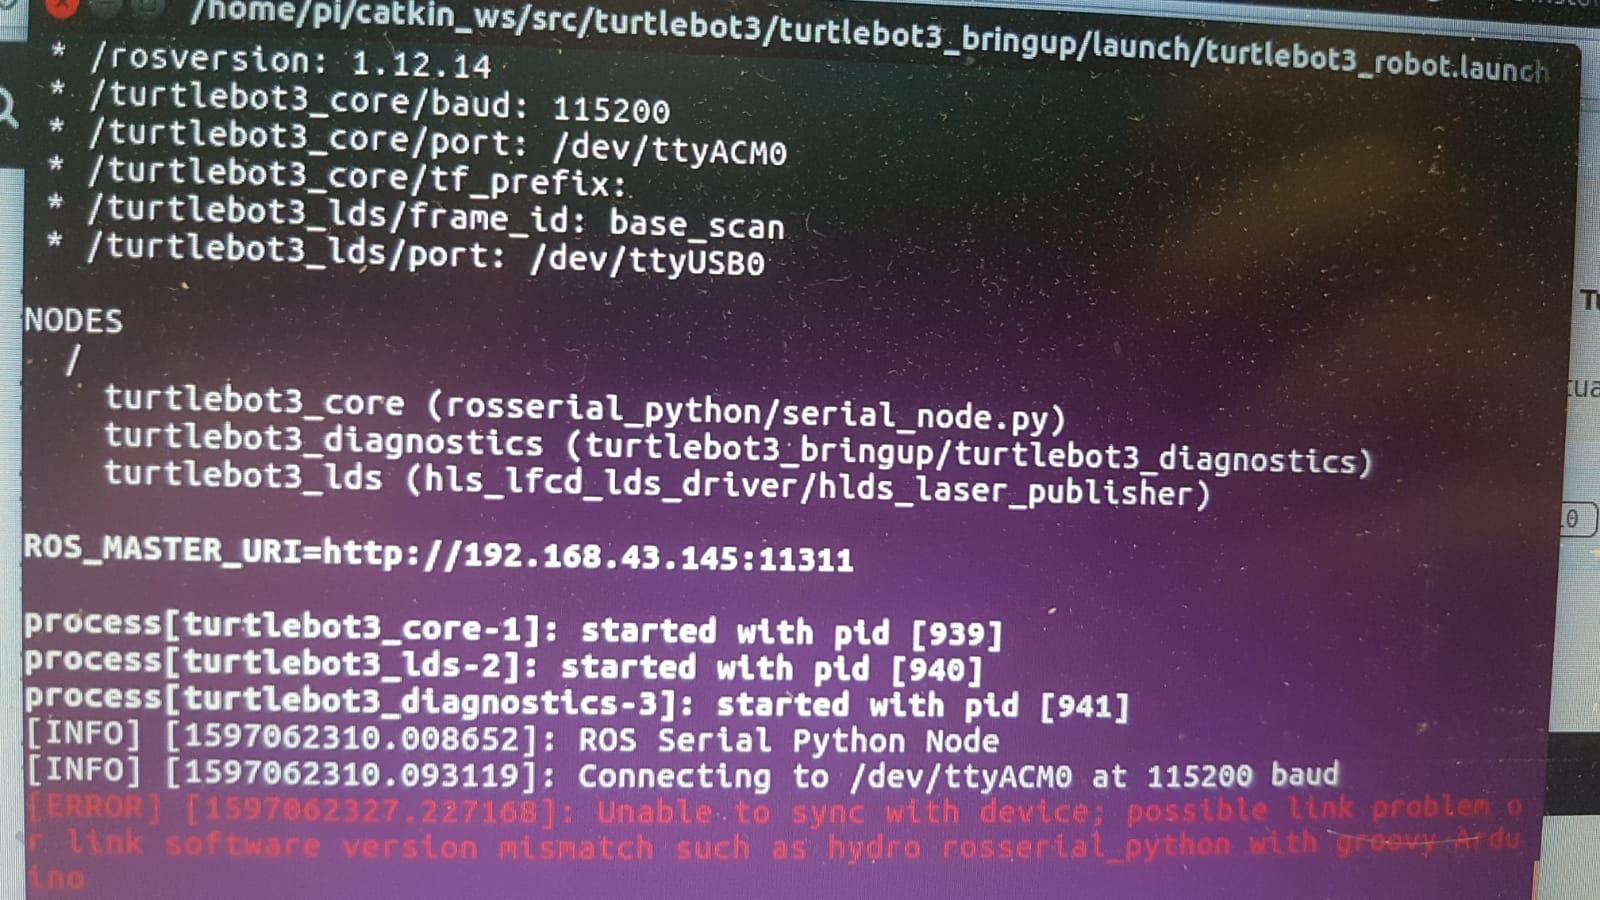
\includegraphics[width=.65\textwidth]{ErrorPhysTurtle.jpeg}
    \caption{Error output after Bringup command}
    \label{fig:errorphys}
  \end{center}
\end{figure}
\label{fig:errorbringup}
\newline
We also tried to put the TurtleBot dimensions in scale to objects to get a better understanding for our developed Use Cases. These can be seen in figure \ref{fig:turtle} and figure \ref{fig:arm}.
\begin{table}[h!]
\centering
\resizebox{\textwidth}{!}{%
\begin{tabular}{|l|l|l|}
\hline
IPS Technology          & TurtleBot3 waffle\_pi             & OpenManipulator-X             \\ \hline
Size                    & 138mm x 178mm x 192mm (L x W x H) & 380mm Reach                   \\ \hline
Weight                  & 1.80 kg                           & 0.70 kg                       \\ \hline
Payload                 & 30 kg                             & 0.50 kg                       \\ \hline
DOF                     & 9 DOF (IMU)                       & 5 DOF (4 DOF + 1 DOF Gripper) \\ \hline
Expected Operating Time & 2 hours                           & -                             \\ \hline
\end{tabular}%
}
\caption{Selected specifications of TurtleBot and OpenManipulator \cite{tbspecificiations}}
\label{tab:specifications}
\end{table}

The overall impression of the physical TurtleBot3 was that it was quite stable so that lifting objects and transporting objects should be possible. The TurtleBot3 itself has a payload of 30 kg and the OpenManipulator 500 g \cite{tbspecificiations}. \\
However, within the 30 kg payload it needs to be considered that components like the arm (700 g) and additional sensors and hardware also need to be deducted from the payload of the TurtleBot itself.\\
Though its small payload, the OpenManipulator itself was quite flexible and that the joints could be moved without any difficulties in different directions. It was also able to touch the floor so it could possibly lift up objects.\\
\newline
Furthermore, the TurtleBot3 is designed in a way that it is easily extensible by further components such as sensors and also it's height could be easily increased in this manner.

\begin{figure}[h!]
  \begin{center}
    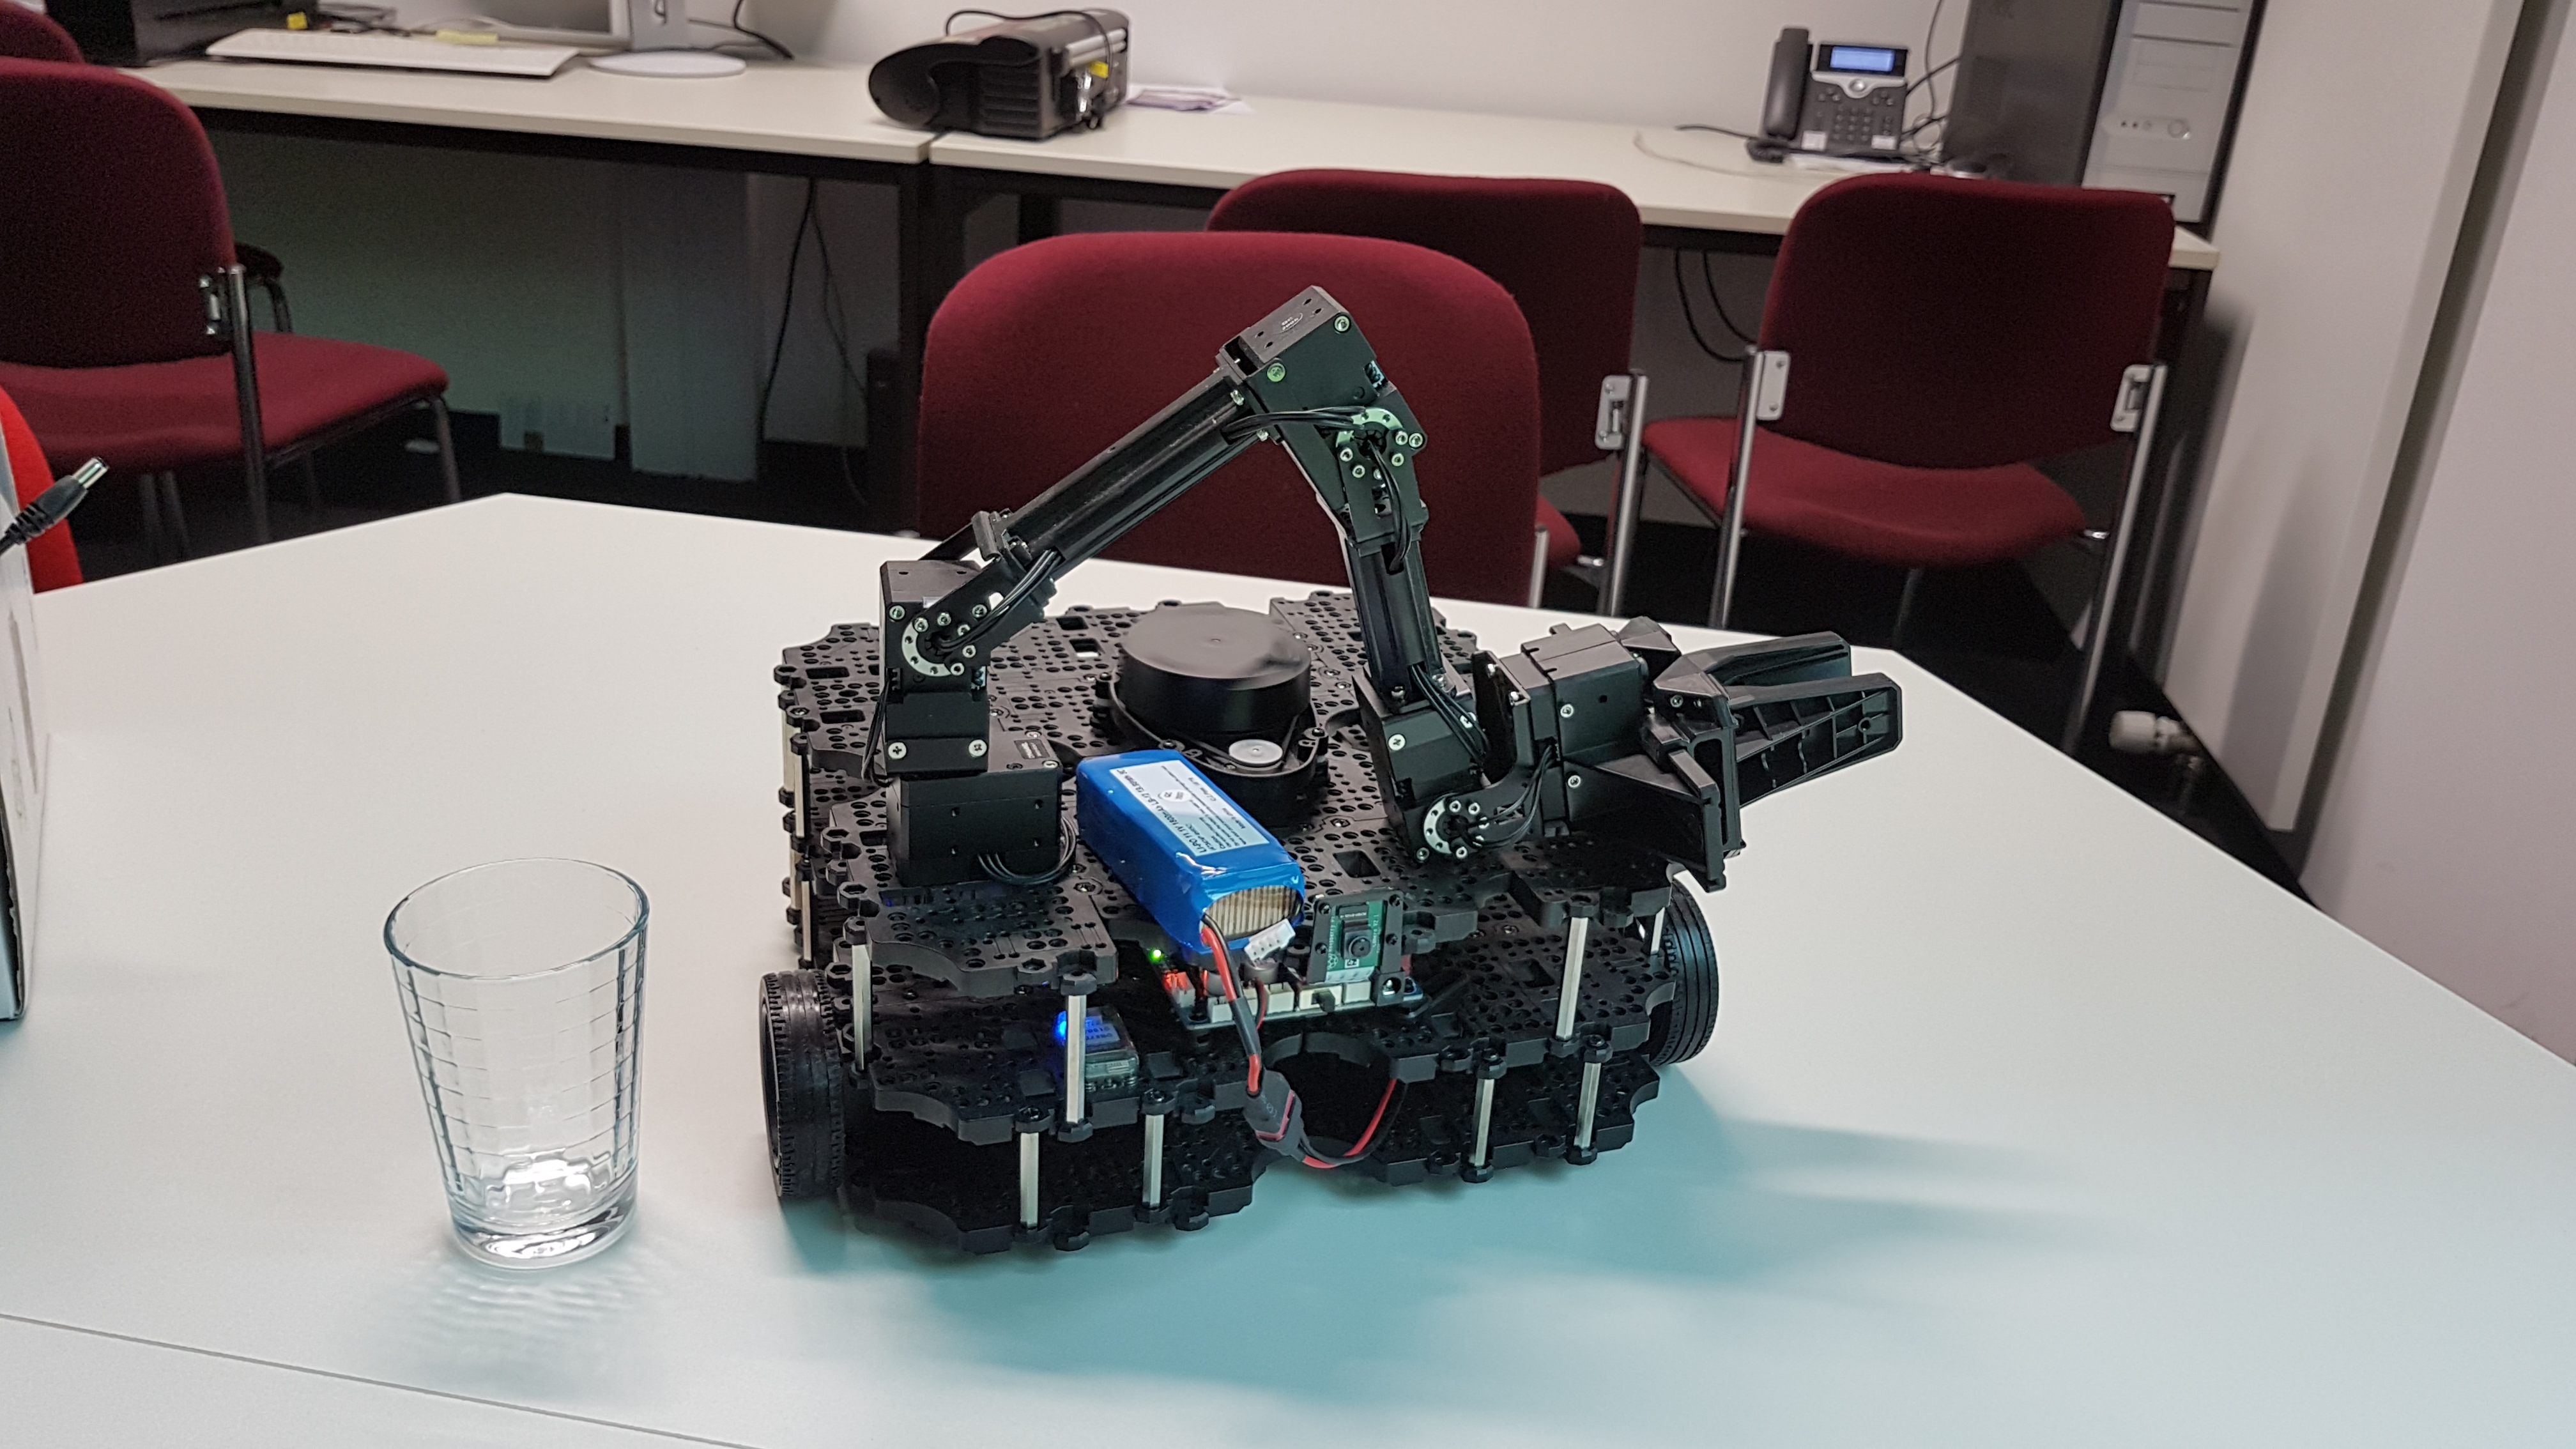
\includegraphics[width=.6\textwidth]{TurtleDimensions.jpg}
    \caption{TurtleBot3 with OpenManipulator-X with drinking glass for scale}
    \label{fig:turtle}
  \end{center}
\end{figure}

\begin{figure}[h!]
  \begin{center}
    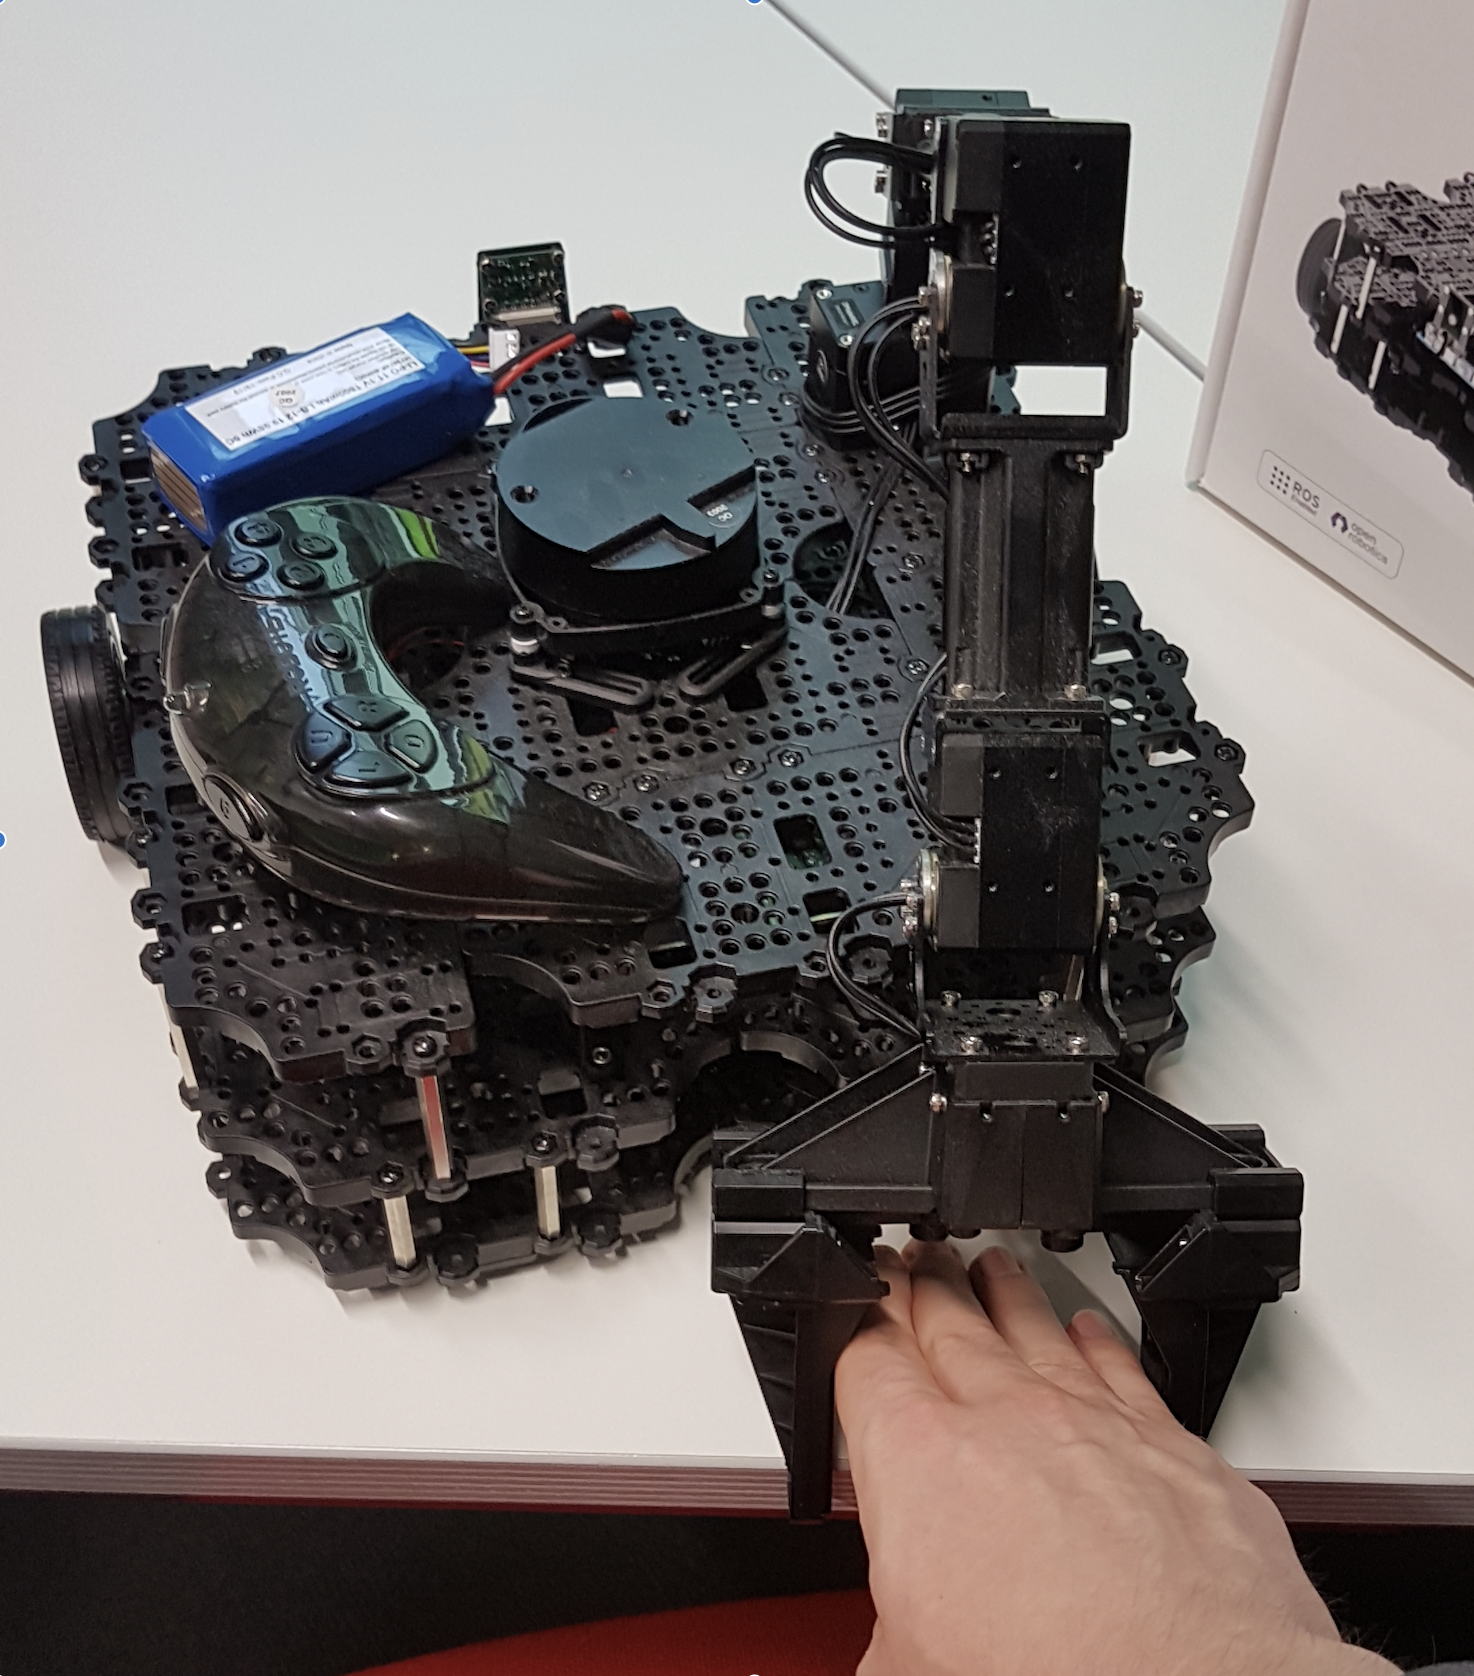
\includegraphics[width=.6\textwidth]{ArmSpannHandQuadrat.png}
    \caption{OpenManipulator-X gripper maximum opening with hand for scale}
    \label{fig:arm}
  \end{center}
\end{figure}


\clearpage
\section{Possible Use Cases}
In this section, possible Use Cases of the TurtleBot will be discussed in order to provide further guidance for their implementation as well as to give an understanding for their theoretical background.\\
\newline
This section is outlined as follows:\\
\newline
In chapter \ref{sec:personas}, three different personas who will be affected by the use cases are introduced. They all have the target group in mind which are elderly people.\\
In chapter \ref{sec:descriptionusecases}, three Use Cases are selected and described in detail. Their theoretical background is based on literature research. Furthermore, the relevance of the use cases for the personas will be determined. Each Use Case will also describe its feasibility of the implementation with the TurtleBot and will discuss whether an expansion of the robot by additional modules is needed. Besides, it will analyze which actions should be performed by the robot.\\
Chapter \ref{sec:sensors} will list the needed sensors based on section \ref{sec:descriptionusecases} and will determine sensor categories as well as any needed additional hardware. Ideal specifications of each hardware module will be described as well.\\
Lastly, in section \ref{sec:conclusion}, the usefulness of the Use Cases as well as their ease of implementation will be consolidated. Additionally, the scope, i.e. how many personas could benefit of the use cases and its scalability will be compared as well.\\
\newline
For the literature research, several search engines such as IEEE Xplore or Google Scholar were used to find relevant papers. The found search of papers was enhanced by reverse search where a closer look was taken at the often cited sources in the initially found literature.

\subsection{Personas}
\label{sec:personas}
According to the WHO \cite{who18}, by 2050, the proportion of elderlys (>60 years) will be almost doubled from 12\% (2015) to 22\%.\\
In high-income nations, this shift of population is especially noticeable. For instance, in Japan, already 30\% of the population are elderly citizens. This trend accompanies several effects such as the issue of the shortcoming of of workers, e.g. in the care facilities \cite{yamazaki12}. The effects of that shortcoming are also noticeable in the results of the interviews in section \ref{sec:appendix}.\\
These ongoing trends underline the relevance of the later discussed Use Cases and reflect that trend.\\
\newline
The personas selected have health conditions that are common within the aging population such as cataracts, back and neck pain. Often, several conditions happen at the same time \cite{who18}. The persona's description and symptoms are based on selected personas from MOOCAP \cite{moo}. They were altered however so that they fit the intended target group (e.g. age). Further, the descriptions focus on the relevant parts as MOOCAP was written with a focus on personas using the computer which is not as relevant for assistant robots. The here described personas are written so that the general impairments in their daily life become clearer.\\
\newline
As a general guideline for finding needed properties for each persona, four categories were defined: \textit{Background of the person} (e.g. what the person did as a previous job, living conditions), \textit{Demography} (e.g. name and age), \texit{Identifications} (e.g. health conditions, symptoms, hobbies, interests, attitudes) and \textit{Problems in Daily Life} (e.g. due to the health conditions).\\
The personas from MOOCAP were selected and the information was classified into these categories. Afterwards, necessary further information was brainstormed based on experiences as working in a hospital and used to enrich the described personas. To properly address the health conditions, information on them was researched in literature as well. Finally, the found categories were consolidated and linked. \\
The last persona, Lisa, was invented in order to have one supporting persona to be also able to address the needs of the opposite site, the people working with the elderly in order to discuss effects like the shortcoming of workers. She is based on experiences with hospital workers.
\newline
For further research, a refinement of those personas is needed by further empirical research. The sample size of the interviewed personas is not representative. Deeper interviews and also interviewing elderly people themselves were not possible due to time constraints.

\subsubsection{Gertrude, 72 - Visually impaired}
\label{sec:gertrude}
\begin{figure}[h!]
  \begin{center}
    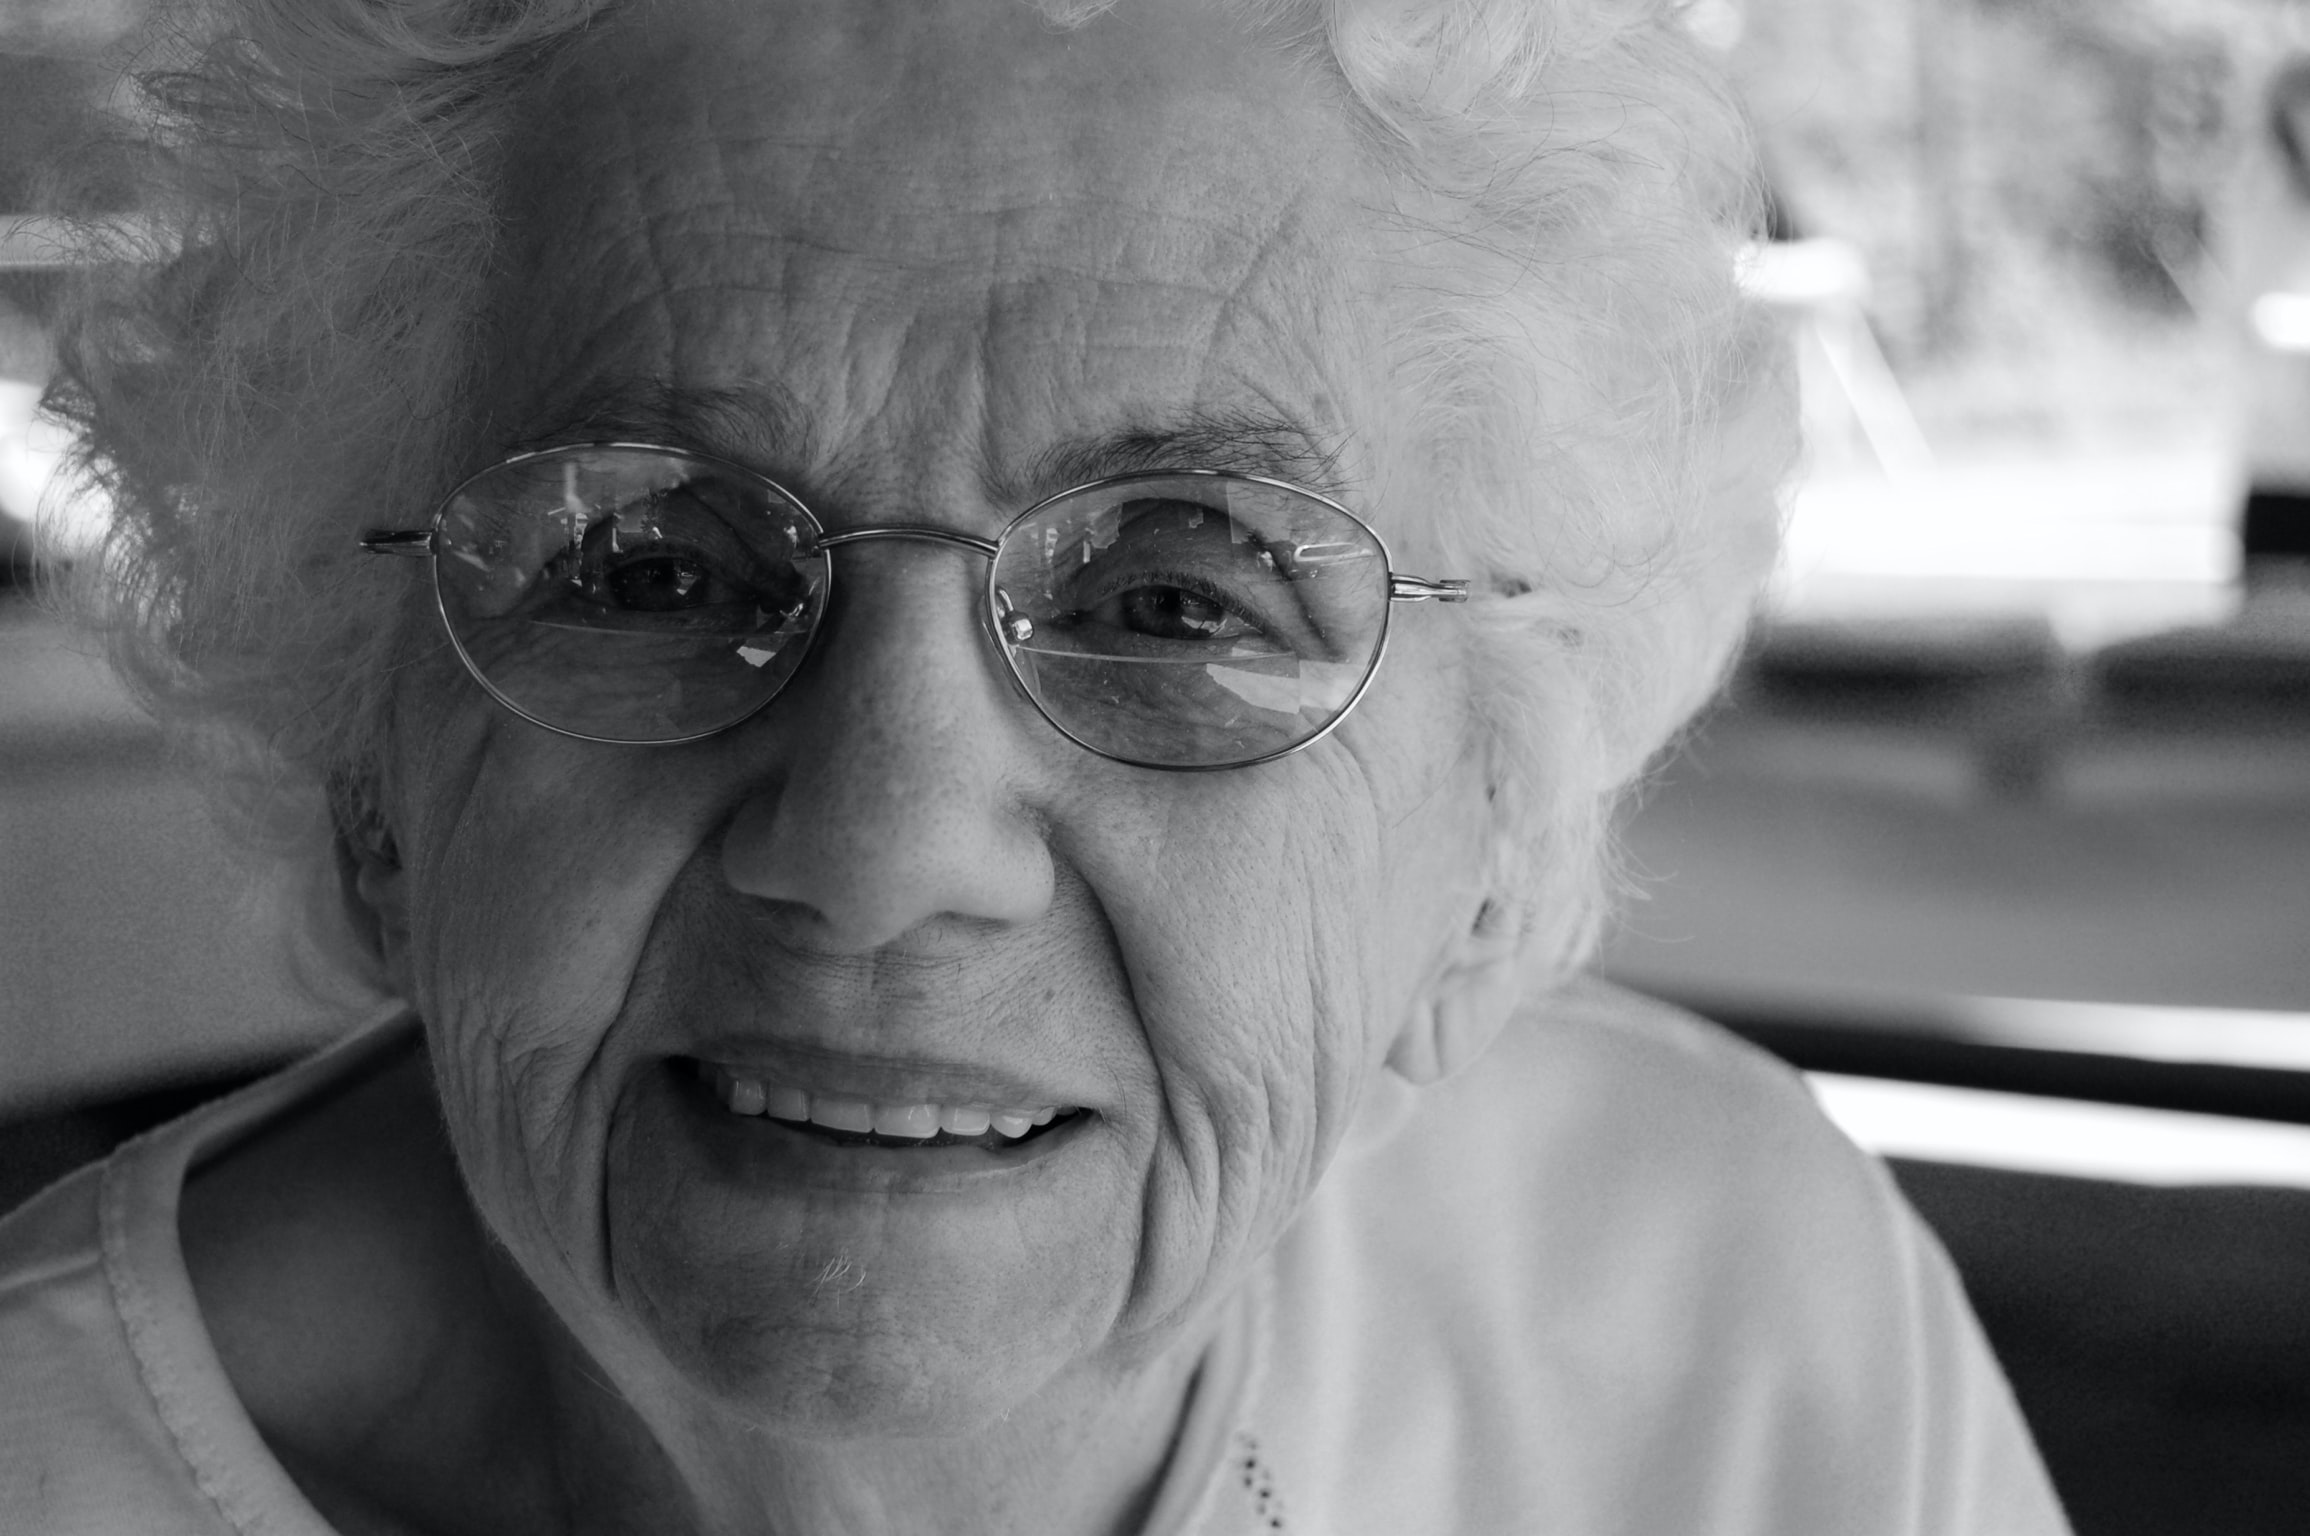
\includegraphics[width=.65\textwidth]{gertrude.jpg}
    \caption{Gertrude, 72 \cite{gertrude}}
    \label{fig:gertrude}
  \end{center}
\end{figure}
\emph{This persona is based upon the persona Monika described in MOOCAP \cite{monika}, her age was altered since our age target age group are elderly people affected by their age. Her illness was changed from macular degenaration to cataracts since cataracts is statistically more prevalent among the elderly generation.\cite{Klein1982}. \\
\newline
Furthermore, Moocap added some more information on how Monika interacts with the environment outside of the comfort of her home. The difficulties she has within her home, her past life and also details about her personality and how she spends her time at home as well as the relationship with her family and friends were not discussed as much in Moocap, so it was decided to enrich Monika with that information. This information is based upon personal experiences with patients who cannot be disclosed due to data privacy reasons.}\\
\newline
Gertrude (figure \ref{fig:gertrude}) is 72 years old and lives on her own in Dresden. She lives in a house with a conservatory at ground level.\\
Gertrude is retired but would like to be as independent as possible. When she was young, she worked as a nurse. Her husband died ten years ago. Her family lives far away in Stuttgart. She has two kids and four grandchildren.\\
Gertrude is still physically active, however, she runs quite slowly. She loves working in her conservatory and arranging the plants there. Additionally, she is a passionate cook. She uses public transport for shopping.\\
\newline
Gertrude is visually impaired as she has cataracts. Due to that, her lenses become cloudy and she tends to have a blurry and less colorful vision. She is also very sensitive to light and has bad night vision \cite{aao19}. 
Furthermore, her spatial vision is affected as well.\\
Cataract can be healed by an operation, which exchanges the lens. However, Gertrude is afraid of complications so she tries to delay it as much as she can. Her doctor says that if the illness is not disturbing her too much in her daily tasks, she can wait until later for surgery \cite{iqwig19}.\\
So far, she can handle most of her tasks without too many issues. She does not want to have a caregiver as she wants to be independent and handle tasks on her own.\\
However, she used to prefer the traditional way over the digital one. For instance, she used to go to the bank office's ATM to handle financial affairs. It closed some time ago so she needs to either travel to the city or use online banking. Due to the complex menus and risks she heard about online banking, so she tries to avoid it.\\
\newline
In her home, sometimes, however, she hits the door frame when she wants to go to the toilet due to her bad spacial vision. 
When working in her conservatory, Gertrude has issues to find the right plants and tools when the sun shines to bright. She also has difficulties to read texts such as tags on her newly bought plants or recipes for cooking.\\
Gertrude also tends to feel very lonely as her family rarely visits or calls her. She wishes to see her grandchildren again and to play with them. She remembered that she told them a lot of stories of her past and also read books to them. Also, she wishes to talk more to other people but most of her friends either moved away or have died.

\subsubsection{Dieter, 82 - Mobility impaired}
\begin{figure}[h!]
  \begin{center}
    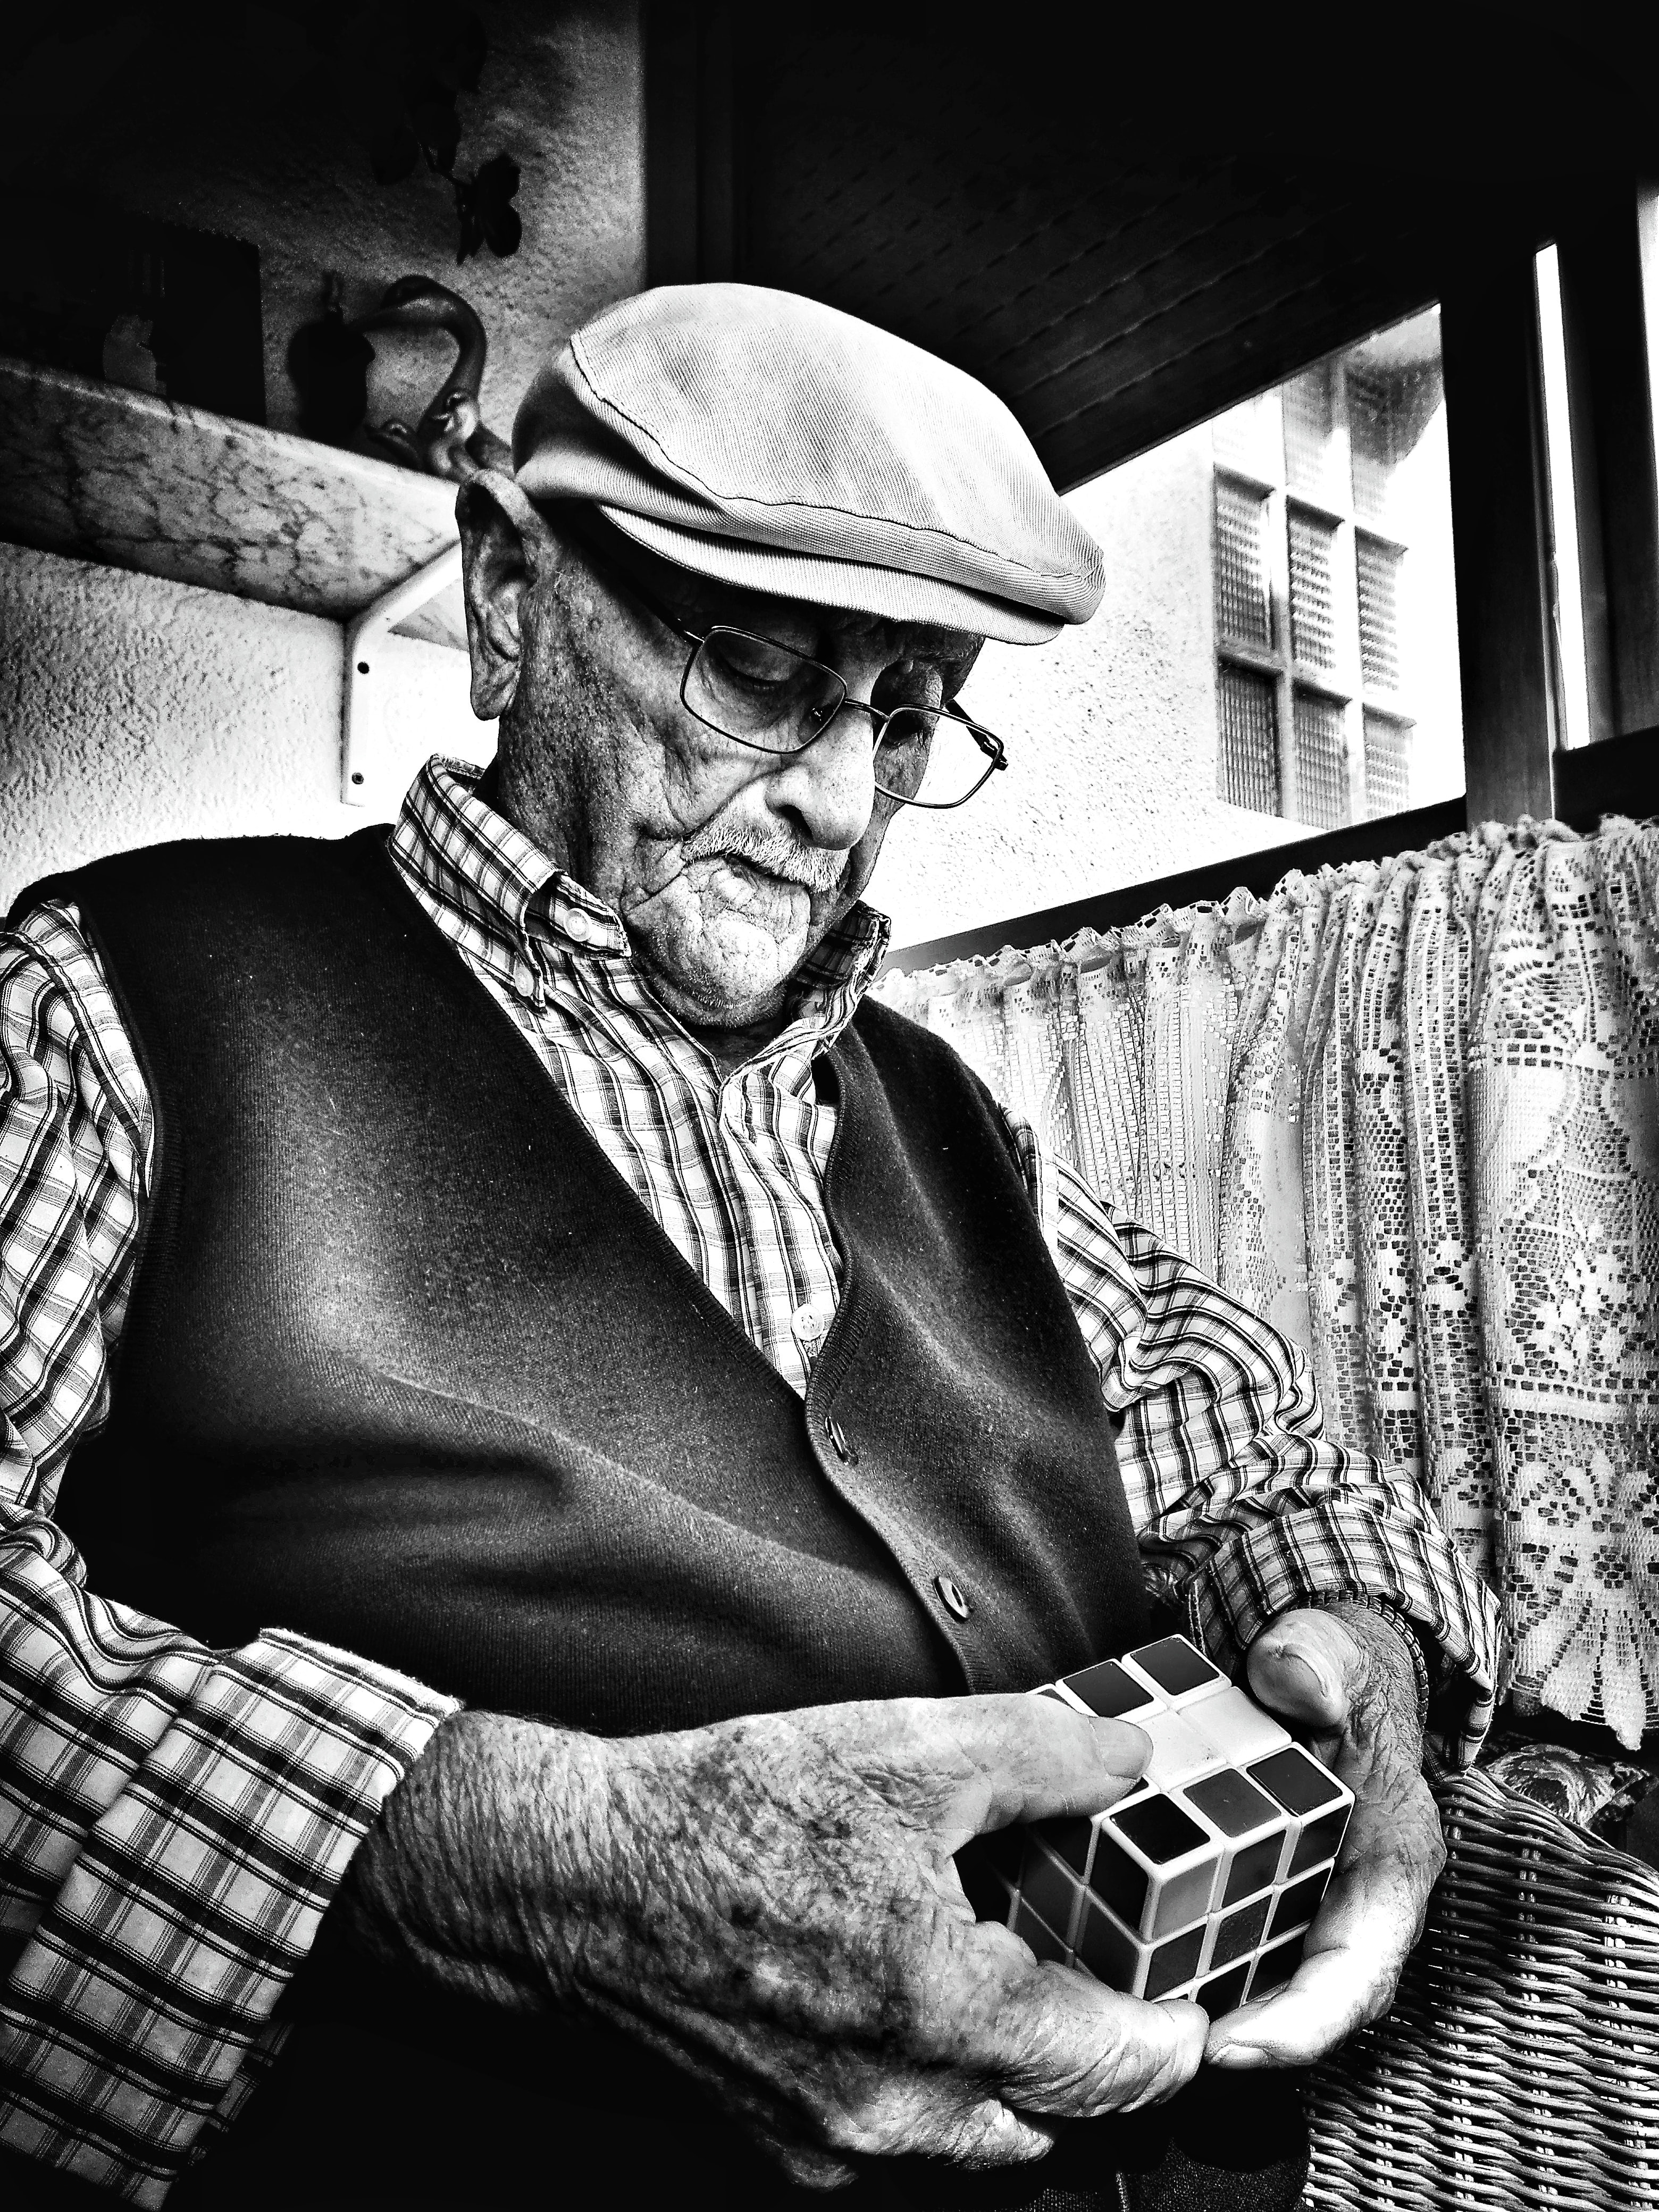
\includegraphics[height=.65\textwidth]{Dieter.jpg}
    \caption{Dieter, 82 \cite{dieter}}
    \label{fig:dieter}
  \end{center}
\end{figure}
\emph{Dieter is based upon  Mary \cite{mary} from MOOCAP and some information about Mary was altered to better fit the needs of this paper. First of all, the gender and age were changed. The gender was changed so that a variety in genders in the selected personas are available. Secondly, the age was changed to fit the intended target group of retired seniors.\\
\newline
Thirdly, the illness was changed from rheumatoid arthritis to osteoarthritis. Osteoarthritis is the most common joint disease amongst elderly people. About 80\% of the seniors are affected by this illness. \cite{ARDEN20063} \cite{rheumanetz}.\\
Both diseases are similar in their symptoms, however, Osteoarthritis is "caused by mechanical wear and tear on joints" while "Rheumatoid arthritis is an autoimmune disease" \cite{healthwise}.\\
\newline
Thus, the symptoms from Mary were taken into consideration for Dieter as well. However, as Mary is not yet retired, the circumstances in which the symptoms occur are different. In MOOCAP, the symptoms of Mary were described in the context of her working environment such as working on a PC. However, Dieter is retired and thus he will experience these symptoms in his daily life. In MOOCAP, the hobbies of the persona were not described, as there was a focus on the interaction with a computer at her job. Hence, the persona needed to be enriched with that information as well as with a personal background and relationship with family, as these are relevant for the use cases. Furthermore, Mary's job needed to be changed as it includes modern technology which was not in use at the time of Dieter's career.\\
\newline
This enriched set of information is based upon personal experiences with patients.
}\\
\newline
Dieter (figure \ref{fig:dieter}) is 82 years old and lives alone in his own house in Dresden. \\
Dieter wants to be as independent as possible even though his family does not live with him. Furthermore, his wife died 3 years ago. When he was still working, he used to be a locomotive driver. Now, he enjoys working on his model railway in his garage where he spends the majority of his time. When he does not feel well, he watches train documentaries on his TV.\\
\newline
Dieter has Osteoarthritis \cite{arthritis}, the most common type of Arthritis which affects mainly people older than 50. Due to that, his fingers and knees feel very stiff, especially in the morning. He also has problems to bend over. His symptoms vary each day. Sometimes, it is very hard for him to wake up. Additionally, his fingers tend to swell. For this reason, he often drops material when he is working on his model railway. His fine motor skills also got worse over time so now there are some gestures, he cannot do anymore such as picking up or adjusting smaller items.\\
\newline
As his conditions make movements quite exhausting for him, he prefers to not move to much and he does not exercise at all. When he was younger, he used to go for a walk outside but now his knee and feet pain got worse over the years.\\
His lack of exercise did lead to more conditions such as high blood pressure. When it gets worse, he feels quite dizzy and his fingers shake \cite{osthoff19}. However, these symptoms seem to be quite stable over the last year.\\
\newline
To make sure that he is fine, he has a care assistant who looks after him daily. She cooks for him and also brings him his medicine against his illnesses. In his whole life, he never cooked as his wife used to do it for him. After she died, he needed a caregiver to do it as it was hard for him to operate with the tools such as the knife. His wife also controlled that he takes his medicine as Dieter tended to forget it. Now, his caregiver has to do it.

\newpage
\subsubsection{Lisa, 45 - Nurse at an elderly care home}
\label{sec:lisa}
\begin{figure}[h!]
  \begin{center}
    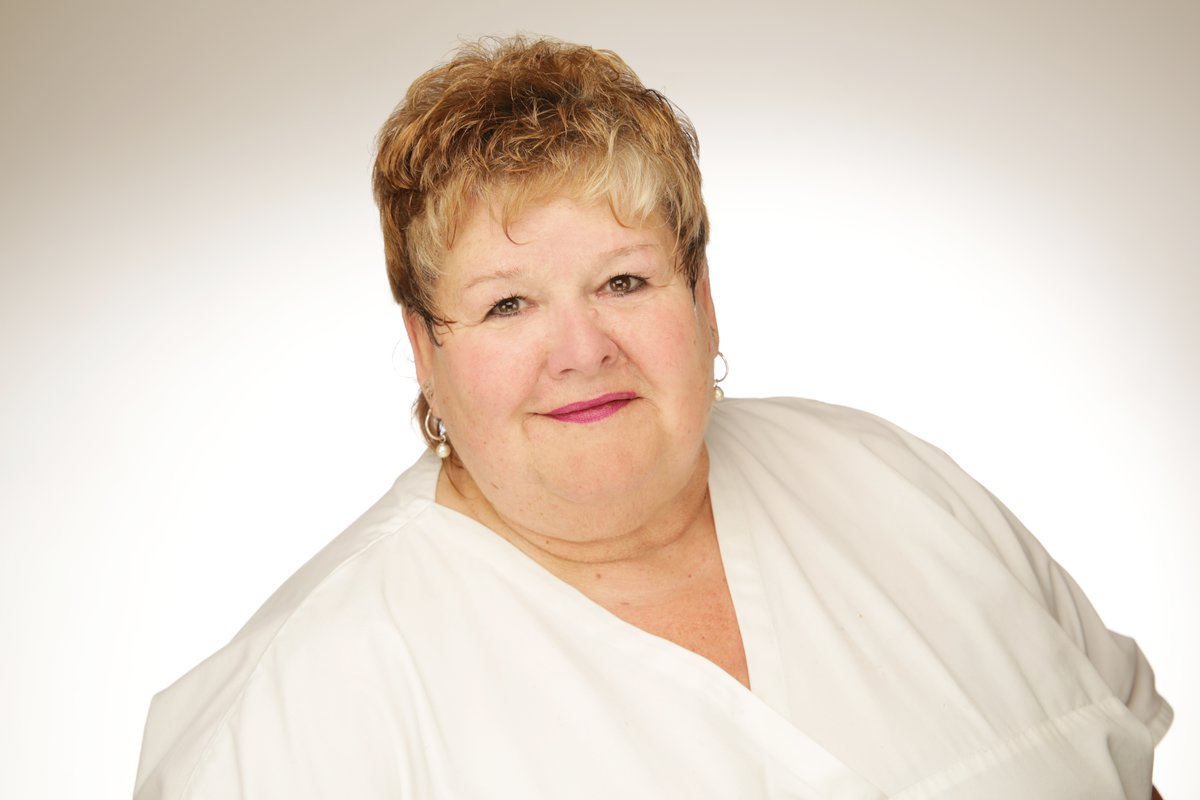
\includegraphics[width=.6\textwidth]{Lisa.jpg}
    \caption{Lisa, Nurse at an elderly care home \cite{lisa}}
    \label{fig:lisa}
  \end{center}
\end{figure}
\emph{This persona is based upon a real life person, all aspects described here denote from her personal experiences. Due to anonymity reasons, her name cannot be cited here.}\\
\newline
Lisa, a 45-year-old nurse, has been working as a nurse in an elderly care home for approximately 10 years now and is a single mom. She lives in an apartment in Dresden with her daughter which she sees rarely due to constant overtime due to a lack of staff being on call. On the weekend, she enjoys some active outdoor activity such as hiking and spending some quality time with her daughter. Furthermore, she needs any free days to rest and catch up on missed sleep due to heavy work hours. \\
\newline
She is chronically tired since she has to work so much, and like many nurses she is under a lot of stress due to a staff shortage, which affects her overall well-being \cite{shapiro2001nurses}. The constant lifting of patients and bending down has put a strain on her back, leading to pretty regular back pains and a general stiffness in the back area which is a common back injury in the nursing branch \cite{doi:10.1002/nur.4770100106}. 
This leads to pain when she strains her back too much or makes walking sometimes painful.\\
\newline
Due to a general lack of nursing staff, a lot of the staff is overworked including Lisa which leaves little time for breaks. She wishes daily for some kind of additional support may it be through new hires or newer technologies. Many of her daily tasks are quite repetitive, such as handing out medicine or changing the bedding of patient.\\
\newline
Lisa has a strong ethical and moral compass which she applies as work, patient care for her is not only a job but also a vocation. It is for her of utmost importance that the rights of her patients be respected.\\

\newpage
\subsection{Description of Use Cases}
\label{sec:descriptionusecases}
In an aging society, there are several effects according to Yamazaki et al.: "A declining population, an increasing proportion of seniors and changes in family structure" \longcitesingle{yamazaki12}{2429}. These are all issues that can be solved, according to the authors, with assistive technology. They categorize the support in three major categories: Labor support to overcome the issue of the shortcoming of workers, healthy lifestyle support and household and care support. These categories are also visualized in figure \ref{fig:yamazaki12}.\\
\begin{figure}[h!]
  \begin{center}
    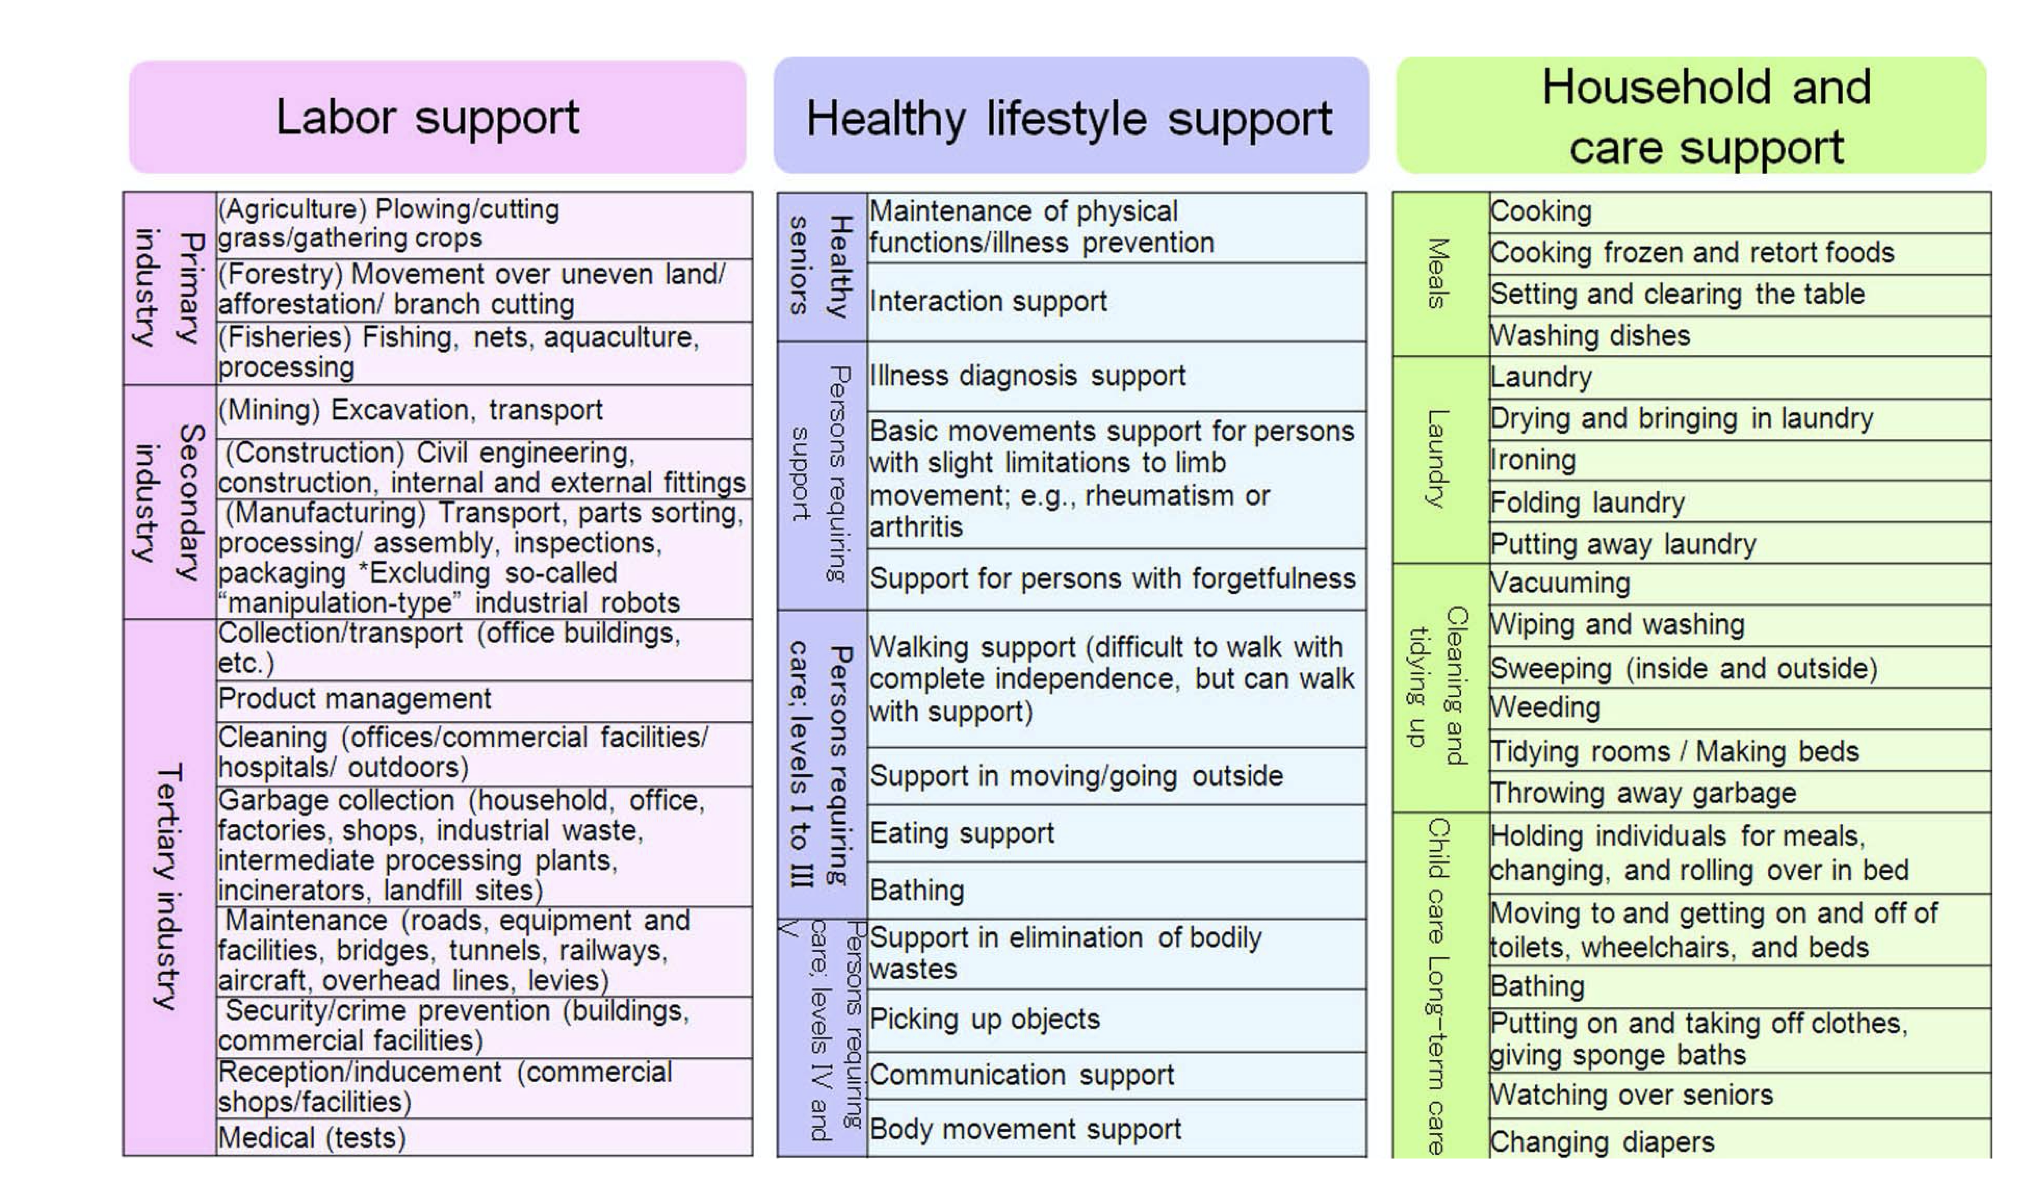
\includegraphics[width=.95\textwidth]{robot_categories.png}
    \caption{Overview of specific tasks and supporting technologies \shortcitesingle{yamazaki12}{2430}}
    \label{fig:yamazaki12}
  \end{center}
\end{figure}
\newline
These defined categories can be used as a guideline to define specific use cases. Their relevance is determined by the special needs of the personas. \\
\newline
However, Yamazaki et al. \cite{yamazaki12} did not define in particular the role of the robot as a personal assistant. However, as Hutson et al. \longcitesingle{hutson11}{578} point out, the existing literature mainly focus on the "healthcare and healthy behavior among the elderly". This would be categorized in the category \textit{Healthy lifestyle support} according to Yamazaki et al. According to the National Institute of Aging \cite{nia19}, there is a connection between social isolation, loneliness and several physical and mental conditions such as high blood pressure and cognitive decline. This shows that there is a need for counteracting this loneliness. Thus, we identified that the use case socializing, in particular with the goal to decrease the feeling of loneliness is relevant to be tackled as a use case. Hutson et al. \cite{hutson11} identified that robots have the potential to improve the well-being of the elderly which goes further than only the identified \textit{healthy lifestyle support} by Yamazaki et al.  \cite{yamazaki12}. Hutson et al. discussed several requirements to be met for a social robot so that they can decrease the feeling of loneliness and therefore improve the elderly people's well-being. These requirements will be objective of section \ref{sec:socializing}. \\
\newline
Transportation of medication is an important part of the daily care taking process. The overall increasing age of the population and less people pursuing the nursing profession leads to overwhelming nursing facilities and stressed out caretakers \cite{yamazaki12}. The solution is that robots can be used to conduct physical labor, therefore helping caretakers by performing automated, mundane tasks. This frees their hands and allows them to focus on other, more complicated tasks. While the main benefactors of these robots are mainly caretakers like Lisa (\ref{sec:lisa}, the overall changes in the nursing home also indirectly affects inhabitants. This use case will be further discussed in section \ref{sec:transporting}.\\
\newline
As see in figure \ref{fig:yamazaki12}, under the category 'Healthy lifestyle support', 'support in moving' is an issue which can be solved with assistive technology.
A guidance robot, also more commonly known as Electronic Traveling Aid (ETA), have been used widely to assist blind people. The use of robots to help the visually impaired is a relatively good alternative to guide dogs, especially indoors for people with either an allergy or for people which would be incapable of taking care of a pet \cite{Alhmiedat2013}. Therefore, underlining the usefulness of a relatively low-cost guiding robot. A Persona such as Gertrude (\ref{sec:gertrude}) could benefit from such a robot.
The use case will be further detailed in section \ref{sec:guiding}.
\newline
\subsubsection{Transportation \& Picking up - Carrier}
\label{sec:transporting}
Transporting and Picking up objects is a field which focuses on automated physical tasks. Robots are capable of performing distinct actions. In the context of figure \ref{fig:yamazaki12}, a robot can perform tasks for tertiary labor support by collecting and transporting objects or as healthy lifestyle support by picking up objects from the ground. For both tasks aging plays a central topic. With an increased age, human face additional issues especially when carrying out physical tasks like picking something up from the ground. A robot hereby has the potential to become a physical extension of the human. An increase in the elderly filling nursing facilities and additionally a shortage in people pursuing the nursing profession also leads to existing caretakers being understaffed and overwhelmed by their task schedule. \\
\newline
In our conducted interviews \ref{sec:appendix} a positive response was received for a helping robot, which transports medication and medical equipment to the right places. This would help them reduce task load and stress significantly, while also giving them more time for other tasks.
Therefore the proposed use case will be to carry and distribute medication and other medical equipment to specified places in the facility. To incorporate the OpenManipulator arm, there will also be a 'giving out' task, where the TurtleBot gives the right object to the recipient.
The use case can be further divided into sub tasks, which will get briefly discussed in regards of functionality and concerns.
\begin{enumerate}
    \item \textbf{Mapping of medication to the recipient}: Care takers need to be able to plan out, which inhabitant gets which medication. The robot needs to recognize this assignment somehow. One possibility is to use designated slots in a special casing, where medication can be placed into. Through an interface the care takers can now determine the slots for the recipients. Another way to map is to use a camera, which points to the payload area. With this camera newly added drugs can be registered and assigned.\\
    \newline
    One problem of this lies in the liability of such a setup. When handling prescriptions it is important that the process is as error prone as possible. While human error especially in such a stressful work environment is inevitable, in the conducted interview one nurse was concerned with the legal handling of errors caused by the robot. This topic is very extensive itself and will therefore be not further discussed. \\
    \item \textbf{Plan routes to recipients}: Planning out a route can either be done manually by the care taker or automatically by preexisting pathing algorithms. Fung et al. \cite{Fung2003} mentioned that in an automatic approach the robot should be able to find an optimal path, which is done based on already available map data. The actual navigation could for example be achieved by using natural landmarks in the hallway like florescent lamps in Fung et al. or predefined paths visible on the ground. The problem with the latter is obstacle avoidance, because the path has to be detected again. Further navigation possibilities will be discussed in the use case Guiding \ref{sec:guiding}.\\
    \item \textbf{Carry and navigate hallways}: Carrying and transporting the payload is going to be the main task of the robot. Here several concerns have to be considered. Firstly the payload has to be secure. Medicines should be fixated in a designated place and should not move even while the robot is turning. Fung et al. also proposes to use a locker with password to eliminate malicious attacks on the payload. \\
    \newline
    Because corridors are usually narrow and might be busy with people, the robot should actively avoid obstacle like objects and humans to guarantee safety for everyone. Especially the elderly might not see the robot, which also needs to be further addressed. A solution to this is to make the robot appear more human. This not only raises awareness, but also adds familiarity instead of an alien robot, where there is no association. Ljungblad et al. \cite{Ljungblad2012} focused in their study on the reception and reaction of the public in a hospital upon seeing a transport robot. They describe an \textit{Utopian Model} where familiarity and time directly influence the perception, which might range from an alien to a working colleague. For example working and interacting directly with the robot steadily improves his reputation towards the person compared to a worker who is only seeing the robot in passing. \\
    \item \textbf{Deliver and give out medication and supplies}: The robot needs to come drive into a recipients room and deliver the designated object. A main concern is that elderly might not want to take medicaments or are not familiar with the robot even after tutorials by the care taker. Zhu et al. \cite{Zhu2012} developed for this reason etiquette strategies for human-robot interaction. Here an interesting strategy is for the robot to leave the room after entering while the recipient is playing for example a game to establish politeness. They also mentioned an etiquette model which splits linguistic politeness into different levels, which are indirect hints, concise requests, compliments or apologies, applied them to the robot and directly compared them on perception and effectiveness. The result was that the lowest response time and the highest score was achieved by the apologise strategy. This study builds a good foundation of robot etiquette.\\
    \newline
    The delivery can be done in various ways. The simplest solution is that the recipient just takes the medicament manually and then presses a certain button or interface to let the robot know that he can continue. Another solution would be to use a robot arm to grab the medicament and either place it into the hand of the recipient or put it on a table. This method adds a lot of complexity, because arm movement has to be very precise and medicament dimensions have to be taken into account. If there is no arm available and the drugs are saved in a locker, there could also be distribution akin to getting a drink from a vending machine, where the target medicament gets put out in a collect area.\\
    \item \textbf{Start, stop, continue and homing mechanisms}: The robot needs a mechanism so care takers and recipients can manually control the schedule. There should be an interface, which lets the robot start, stop and continue a delivery task, so the robot understands when a care taker is done stocking the medicine, when there is a problem in the process or when he needs confirmation that he successfully delivers one medicament. \\
    \newline
    Additionally a homing function is necessary to return to the starting position after fulfilling all the delivery tasks. Following the path algorithms discussed above, this should not be problematic and would just add another checkpoint.
\end{enumerate}
\Paragraph{Limitations of the TurtleBot}
\bigskip
Now that the use case was discussed, the shortcomings that the Turtlebot has for carrying out the specified task are described.\\
\newline
The TurtleBot's main limitation comes with its dimensions. Especially the height makes it difficult for caretakers to stock the robot up or inhabitants to take the medication, compared to already existing transport robots, which people can interact with effortlessly. Another issue is a missing platform to put the medication. Currently there is no extra space on the Turtlebot next to the OpenManipulator and LIDAR sensor. Because the Turtlebot has incredibly small proportions and is therefore hard to see, it might become a liability and even a health hazard in busy hallways as pointed out in Interview A.1. Additionally robots like these are limited in the space that they can explore and can not operate multiple floors without an elevator or manual help.\\
\newline
Other specifications, which can be found in table \ref{tab:specifications}, can also be problematic for the viability of the TurtleBot. While the maximum payload weight of 30kg is more than enough to carry medication in most cases, the OpenManipulator can only lift objects that are 0.5kg or under. Especially if the arm is used to give medication to the right people, this could be potentially problematic, when the medication weighs more. Medication can also come in various forms and shapes. The gripper of the arm might not be viable for some of these medications to grab them without errors. Lastly the TurtleBot lacks a user-friendly interface, making it hard to for example map the medication with the right location. Through necessary hardware and component additions, these problems will get mitigated, making the TurtleBot a viable solution for small carry tasks. \\
\newpage
\subsubsection{Socializing - Listener}
\label{sec:socializing}
For Socializing, there are different approaches which can be differentiated. In particular, a robot can be used to communicate with others (e.g. the care assistant or family) or the robot becomes social itself and interacts with the user. For this use case, the latter will be considered. In the interviews (section \ref{sec:appendix}), nurses were asked about whether they would consider a robot which is used for communication between them and patients useful. Most of them shared the opinion that it would not help them as much. Therefore it was decided to change the focus more on the aspect to diminish loneliness of elderly people rather than aid communication within a care facility.\\
\newline
In literature on the other hand, it has been discussed that a social robot can help to improve the well-being of elderly people. This is also the goal for a socializing use case. There are several possibilities to achieve this such as  general companionship to decrease the feeling of loneliness or by providing mental challenges and interactions \longcite{hutson11}{581f.}.\\
\newline
For Socializing, the concrete use case, \textbf{Listen to the elderly person} is discussed. 
Hutson et al. \cite{hutson11} suggested that the well-being of elderly people is improved when they have someone to talk to. This might decrease their feeling of loneliness. A robot could be used for this purpose. The acceptance of users for actually using the robot increases even more if they get the feeling that they are doing something good. For instance, telling a story that is forwarded to their grandchildren or relatives so that they can read it or have it as a memory when this person dies.
\newline
In regards of the personas, this use case can be both relevant for Dieter as well as for Gertrude. Both don't have a family who visits them and both don't have many friends. However, once they get visits, they love telling them stories about their past.\\
Dieter however, has a care assistant who looks after him daily so the feeling of loneliness might not be as realizable as it is for Gertrude as she is independent and does not need and want to have a caregiver. The interaction with a robot might help decrease the feeling of loneliness for her but also for Dieter, especially, when his caregiver is not there.\\
\newline
Hutson et al. \cite{hutson11} also realized in their research when they investigated the reaction of seniors to social robots that many seniors do talk to the robots even though the robot might not be able to respond properly. Thus, they described the robots as companions for the elderly. \\
However, the description of a general companion might require too much functionality that needs to be considered. Thus, the use case of socializing was limited to that the TurtleBot is listening to the stories told by their owner, the senior, and that it is able to react to it. Furthermore, the TurtleBot should be able to save the story so it could read it to the elderly again. The reason for this is that these collection of stories could be used to recall their own history once they get a cognitive disease which affects their memory such as Alzheimer. \\
Once the story are saved, the TurtleBot should be able to record or transcribe the story so it can be send to the grandchildren or relatives. This should increase the feeling of elderly people that they are doing something good and thus increasing their likeliness to talk to the robot. The collected story could be sent to the others either via existing social media channels (e.g. messenger app bot for services such as Whats App or Telegram or social networks like Facebook) or via a dedicated app. However, the format of how it should be received needs to be researched furtherly as it depends on the personal preferences and concerns (e.g. data privacy) of the sender and receiver.\\
\newline
From this general description, the following basic functionality of this use case derives:
\begin{itemize}
    \item Listen to the story of the elderly
    \item React to the story
    \item Save the story, i.e. transcribe and save recording of the elder's voice
    \item Share the story with others over the Internet
\end{itemize}
\bigskip

\Paragraph{Requirements of a social robot}
\bigskip
To further refine the basic functionality, general requirements for a social robot need to be reviewed.
Bartneck \& Forlizzi defined that a social robot needs at least be autonomous, able to communicate, to interact with humans and able to mimic human activity \longcite{Bartneck2004}{591f.}. \\
Thus, the TurtleBot should be able to operate itself without help of a third party such as a caretaker. In regards to the specific use case, the robot should be able to listen to the human and reacting without that another person operates it to perform these reactions. The reactions should be as human as possible so it feels natural. Humans interact in both ways, verbally as well as non-verbally. Verbal communication includes words while non-verbal communication includes sounds, gestures and facial expressions. The robot needs to be able to capture these expressions and also be able to react the same way. \\
\newline
One way to recognize these reactions is to use an approach where emotion in speech is recognized. This can be achieved using artificial intelligence as discussed inter alia by Huang et al. \longcitesingle{Huang2019}{5866} and Nicholson et al. \longcite{Nicholson1999}{290ff.}. The researchers also aimed to consider emotion that is conveyed through non-verbal speech such as sounds. To be able to implement a system that is able to recognize the emotion via speech, the TurtleBot needs to be enhanced by a microphone that is sensitive enough to capture and record the voice as well as to capture sounds the user makes when interacting with the system. It is needed anyway to be able to listen to the story to the elderly and record it. \\
\newline
To capture the emotions, there are also other approaches possible such as a video-based solution which mostly focuses on the face of the user \longcite{Salah2018}{372f.}. To realize that approach, the system needs to have a camera. The TurtleBot uses a Raspberry Pi Camera Module v2.1 \cite{tbspecificiations} with 8 Megapixels and the possibility to record a 1080p video \cite{raspbicam}. It has to be tested whether this camera is good enough to capture the emotions.\\
\newline
To be able to react to the story, the robot needs to be able to mimic the human activity \longcite{Bartneck2004}{591f.}. For instance, if the story is sad or the person expresses a sad feeling, the TurtleBot must in any way also be able to express an appropriate reaction to it. As mentioned above, humans express their emotions verbally as well as non-verbally. 
\begin{itemize}
    \item \textbf{Verbal expression}: This means expressing emotions in words. It might be possible that the TurtleBot makes positive comments when the senior talks to it. For instance "You've made me \textit{feel really good}" when they say a compliment to the robot while telling it the story \longcitesingle{shimanoff06}{21}. To realize that, the TurtleBot needs to be able to talk. By design, the TurtleBot can only make simple sounds like "Beep" tones \cite{tbspecificiations}. However, this does not allow the expression of words. Thus, the TurtleBot needs to be enhanced by speakers that allow this expression.
    \item \textbf{Non-verbal expression}: As discussed at the beginning of this section, non-verbal expression might occur differently. One is the expression via sounds which also go further than the simple "Beep" tones the TurtleBot is able to express. For that, the speakers are needed as well. \\
    \newline
    Humans also express themselves via facial expressions \longcite{Salah2018}{372f.}. The TurtleBot does not have a display that allows to display a face or an abstraction of a face (eyes, eyebrows, mouth). It can be thought of integrating one. It might also affect the perception of the robot. However, it needs to be tested with humans whether this display makes the users more likely to accept and use this robot or if not. Previous research such as experiments with the iCat which played chess with a human and was able to react with facial expressions to the game was able to convey a more engaging experience \longcite{Leite2008}{80-82}. It has to be tested whether this is also true for this use case and the intended target group of elderly people. \\
    \newline
    Lastly, humans also express themselves via gestures. As the TurtleBot has the OpenManipulator arm, it might be able to mimic simple gestures with it to appear more authentic. 
\end{itemize}
Hutson et al. \longcite{hutson11}{581-586} defined more criteria that need to be met by a social robot to be more accepted by the elderly target group. They defined different categories such as \textit{Functional requirements}, \textit{User Experience requirements} and \textit{Maintenance requirements}:\\
\newline
\textbf{\textit{Functional requirements}}
\begin{enumerate}
    \item \textbf{Device should respond to voice or touch}: When the user interacts with the robot, the device needs to respond in any way, e.g. talking back or simpler sounds such as animal sounds.\\
    \newline
    As discussed above, the TurtleBot needs to be enhanced by components that allow both the detection of emotions as well as the response to it. Regarding the response to touch, the TurtleBot is not designed that the user touches them (e.g. stroking it). Therefore, this requirement won't be considered in this use case but the one that the TurtleBot should respond to voice. For that, a microphone is needed.
    \item \textbf{Recognize mood and alter its mood based on the response}: When the robot interacts with a person, it should be able to recognize the user's mood and adjust its own behavior accordingly. E.g. if the person shouts at the robot, it should be able to respond. The response can be quite different depending on the use case and also the user's needs.\\
    \newline
    As discussed, several approaches to recognize the mood and emotions can be taken, based on visual as well as on audio cues. To capture them, a microphone as well as camera is required. The latter is already included in the TurtleBot. For implementation, Artificial Intelligence approaches can be used.
    \item \textbf{Functions to promote well-being}: For instance, facilitating communication with relatives, providing intellectual stimulation or ability to talk to the device for telling stories which are transmitted to grandchildren or other people such as caretakers\\
    \newline
    In this use case, the function that promotes well-being is that the robot functions as a listener who is able to react to stories the elderly person tells so it decreases the feeling of loneliness.
    \item \textbf{Accurate and reliable reminders}: This means that the robot could also remind the user of important events such as taking medicine\\
    \newline
    This can be another use case for itself and it won't be considered in scope of the socializing use case where the TurtleBot takes mainly the role of an active listener.
\end{enumerate}

\textbf{\textit{User Experience Requirements}}
\begin{enumerate}
    \item \textbf{Pleasing to be touched or stroked}: The robot's look and feel should be pleasant for the user. It needs to be customize as each person has different preferences. \\
    \newline
    The TurtleBot is not designed to have a pleasant look and feel. Customization might need to be rechecked with actual testers of the target group. Thus, requirements in regards to hardware modules or software specifications can't be made.
    \item \textbf{Appearance}: The robot should not resemble a children's toy as it might affect the perception of the user itself. For instance, if the robot would look like a toy, third parties might change their perception of the user such as thinking that (s)he is childish. Also, if the robot looks like a familiar form (e.g. a human or an animal), the user might expect the robot behave exactly the same way.\\
    \newline
    The design of the TurtleBot is neither human-like, toy-like or animal-like. Thus, it probably won't be compared to existing creatures. However, its machine-like appearance might not be familiar enough to be accepted by humans. It has to be tested if its appearance has a negative effect on its usage.
    \item \textbf{Personality traits}: The robot should show personality such as humour and curiosity. For instance, some robots in the study made unexpected comments such as "I need a hug".\\
    \newline
    This is important to consider when the reaction mechanism is implemented. The TurtleBot should show some sort of human reactions to the story the senior tells. For instance, it could also start to make some witty comments if the story is funny, to also convey its own personality.
    \item \textbf{Unexpected behavior}: The robot should not be predictable in the actions so the users don't loose interest.\\
    \newline
    This means for the implementation that the reactions by the robot should not be predictable and there needs to be some sort of randomized and unexpected behavior. For instance, if the robot responds via talking or making sounds, it should not say always the same words and make the same sounds but should have an appropriate set of words and sounds that are used in the situation but can't be predicted. It is recommended to test the implementation with the users to research whether this criteria is met.
    \item \textbf{Controllable}: The robot should be controllable by the user such as adjusting the volume of the voice.\\
    \newline
    This can be achieved via different approaches. One is the possibility of including a switch on the TurtleBot or using a remote control. However, the issue with this approaches is that the elderly person needs to be able to operate this controls or be able to reach the switch. Dieter for instance has Arthritis which causes his fingers to swell and thus finely operating might be hard for him on a few days. Gertrude on the other hand also has difficulties with modern technology, so a choice for a very natural interaction needs to be found.
    To avoid this issue, it is possible to also use voice recognition. The person could say "Be a little bit more quiet" and the TurtleBot adjusts the volume of its speakers accordingly. Using voice control is also quite a natural approach for operating the robot for especially elderly people, like Gertrude, who have difficulties in operating a system that is based on a virtual interface.\\
    A microphone is needed to be able to realize this approach.
\end{enumerate}

\textbf{\textit{Maintenance Requirements}}
\begin{enumerate}
    \item \textbf{Continuously powered}: The robot should not need to be charged often and it should be as low-maintenance intensive in that regards as possible. \\
    \newline
    The robots operating time is two hours \cite{tbspecificiations}. That might not be long enough for this use case. Thus, it could be thought of extending the TurtleBot with a battery that allows longer operating hours. Especially when it is taken into account that in the specifications defined by ROBOTIS, the OpenManipulator is not yet considered. It might be that the OpenManipulator shortens these operating hours even more.
    \item \textbf{Robust}: The robot needs to be robust for accidents, e.g. if the user accidently drops a glass of water.\\
    \newline
    The TurtleBot is not designed in a way that prevents damage by accidents as all the hardware is exposed. It might be possible to build a shell around the TurtleBot. However, this also influences the appearance of the TurtleBot which is based on the user's preferences.  As these might vary across people, it won't be considered in this use case as it is also not part of the core-functionality the robot has to provide.
    \item \textbf{Easy interaction}: The robot should not have any small switches that are hard for the user to operate. If a voice is used, it should be as clear as possible.\\
    \newline
    This was also discussed in the "User Experience Requirements". Thus, voice recognition might be one of the easiest interaction solutions, if it is reliable and accurate. Further, it has to be considered for the implementation that the voice which the TurtleBot uses to respond, is as clear as possible and easy to understand. 
    \item \textbf{Weight}: If the robot is in an unfavorable situation or stuck, it should be possible to move it to another place or it should be light enough to lift it without too many issues.\\
    \newline
    The TurtleBot itself has 1.8 kg \cite{tbspecificiations} and the OpenManipulator 700 g \cite{omspec}. It has to be considered that also additional components will be added for this use case which also have an effect on its weight. Still, the robot will probably weight less than 5 kg and thus weight the same as an average cat. Still, for users like Dieter it still might be too heavy. However, the TurtleBot can drive itself. Thus, it is not required by the TurtleBot user to necessarily lift it to different locations.
    \item \textbf{Independent}: The robot should not require too much care or attention of the user.\\
    \newline
    The TurtleBot does not specify particular care that is needed. Still, it might be that there is some effort required to set-up the TurtleBot for the first usage. For that, a care assistant could help the elderly person. After that, the only care that should be needed is the charging of the TurtleBot. It has to be considered by the implementation that there is no additional care effort.
\end{enumerate}

\bigskip
\Paragraph{Further use-case specific requirements}
\bigskip
As the requirements that derive from the theory of social robot have been discussed, the additional needed specifications that are special for this use case need to be considered as well.
\textit{Listening to the story of the elderly} by using voice recognition via a microphone and appropriately \textit{reacting} to it by considering the emotions and the mood were covered already. Still, this use case consists of three further components:
\begin{itemize}
    \item \textbf{Save the story}: The story needs to be saved so it can be recalled by the elderly at any time. For that, a voice command can be used such as "Please tell me the story of my mother". \\
    \newline
    This voice recognition is also needed so that the TurtleBot could react to the story. Thus, a microphone is needed anyway to implement this use case. To find the appropriate story, the user could be asked for a title or the TurtleBot's algorithm could intelligently tag the story with keywords so it can recall the appropriate one. However, to describe a good method for being able to recall the story by the user is not in scope of this paper as it requires testing with the users.\\
    \newline
    For saving the story, different approaches can be considered. One approach could be that the stories are saved on the TurtleBot or that they are saved in the cloud. The amount of storage needed depends on the decided data that should be stored. For this use case, initially, the storage of audio files and their transcription to text are intended. \\
    The TurtleBot allows the usage of a microSD card. If the user wants to store the data in the cloud, i.e. on a WebServer, the TurtleBot has to have a possibility to connect itself to the Internet. For that, the user has to have an Internet connection available at their home. \\
    The TurtleBot can be furtherly connected to the Internet via the Ethernet port of the build-in Raspberry Pi, however, this is not practicable as it would be too much effort for the user to connect it all the time. Especially, for elderly users this would mean that they need to bend over to reach the TurtleBot to connect it to the Ethernet. A better approach would be to use a WiFi adapter that can be connected to the build-in Raspberry Pi. With it, the TurtleBot could be connected to the Internet and upload the stories to a web server.\\
    \item \textbf{Read the story}: The TurtleBot should be able to read the story to the user if liked. It could be possible to just play the audio files but it might be that the users feel uncomfortable hearing their own voice. Thus, the story needs to transcribed. For that, either a own solution can be build or existing solutions such as the Text-to-Speech API by Google could be used \cite{google}. It has to be considered though that the voice used for this functionality is the same that is used for reacting to the user.\\
    \newline
    It could be that the TurtleBot even saves the conveyed emotional information as well and expresses it while reading the story, e.g. by gestures with the arm and the voice. However, as this adds additional complexity, it has to be tested with users if it is needed. It could even lead to an interaction where the roles of the storyteller and listener are switched. When the story was recorded, the TurtleBot was in the position of the listener who reacts. Now, the TurtleBot becomes the storyteller and the elderly person becomes the listener. The TurtleBot could also start adapting its story telling behavior during the interaction. Also, it might be possible that the TurtleBot starts telling different stories for further entertainment. A deeper description of these possibilities however would be also out of scope.\\
    \newline
    For reading the story, additional components that were not already described are not needed. The microphone and speakers were already described as a requirement when the affective reaction was discussed.\\
    \item \textbf{Send the story}: The TurtleBot should be able to send the story to other people such as to the grandchildren. This would allow a connection of the user with the world and the sense that they are doing something good when they use the TurtleBot. As discussed by Hutson et al. \cite{hutson11}, this feeling could be beneficial for the acceptance of the TurtleBot.\\
    \newline
    It has to be determined by the people who implement this use case in collaboration with the actual end users how the files are received and also in which form. For instance, the sender, the elderly person, might have data privacy concerns so that they would not want the upload to a social media network such as Facebook. Also, it has to be determined how the receiver would like to receive this story. For instance, they might want to receive the story as an audio-file so they can listen to it with the voice of the elderly person or they might want to receive it as a text-based message so they can read it, e.g. when they are in a noisy environment. It also depends on the needs of the receiving person, e.g. disabilities such as blindness or hearing difficulties. Thus, further research for the exact specifications is needed.\\
    \newline
    Independently from the actual implementation solution, the hardware requirements are the same whether a audio-based or a text-based solution is preferred. For this component, a microphone to capture the voice is needed. To send it to the end-user, a WiFi-adapter for the Raspberry Pi is needed as well. However, this component does not add any new hardware components that were not yet already discussed in this section.
\end{itemize}

\bigskip
\Paragraph{Limitations of the TurtleBot}
\bigskip
As the requirements of the behavior of the TurtleBot for this use case and also additional hardware was discussed, the limitations of the TurtleBot when this use case is implemented need to be considered as well. These were already briefly described but not consolidated.\\
\newline
The TurtleBot has some general limitations which do not affect this use case directly. For instance, if it needs to be operated within the house, it has to be used on flat surfaces within one level. However, the limitation that plays a crucial role for this use case is the TurtleBot's appearance. The TurtleBot has a very functional look and feel so it does not feel as organic as a robot which looks like an animal. Also, it does not have a face so it might be harder for the users to interact with it. Hutson et al. \cite{hutson11} found that each user has different preferences for the look and feel of a robot but it might be that this robot is too far away from the appearance of a living creature so it might be hard for the users to form an emotional bond with the TurtleBot.\\
\newline
Also, due to this look and feel, it is not really possible to touch the robot in order to stroke it or to have it on the lap when talking to it as it consists of cold, mechanical components. The robot will be always on the floor and the elderly person will be talking "down" to it. It might not be that much of a problem for the users but it has to be tested with them. It might be possible to improve that machine-like look by adding a shell with a soft coating to it and adding a display so it gets a face but each person has different preferences. Thus, a general recommendation that leads to a high acceptance of the TurtleBot with the OpenManipulator arm cannot be made.\\

\newpage
\subsubsection{Path finder - Guiding}
\label{sec:guiding}

\Paragraph{General requirements of a guidance robot}

A guidance robot has as a main task to lead the user to the required destination while avoiding any obstacles. This can be done in an indoor or outdoor environment, either of the use cases require different technologies. However, in both scenarios, the robot should have a map of the area to navigate within its memory may it be acquired through data exchange or through self-exploration similar to the technology used by vacuuming robots (cite paper vacuum robots).\\
\newline
As mentioned by nurse in the interviews carried out for this paper in \href{sec:appendix}{section 8}, navigating a complex area can be especially difficult for elderly people. This can be due to many features, either through physical limitation such as visual acuity or due to degrading mental faculties. Helping elderly people get around definitely increases their independence, helping them to lead a more fulfilling life and avoiding unnecessary injuries by circumventing any obstacles a person could oversee and trip upon.\\
\newline
In this use case we will focus on indoor guiding since the wheels of the TurtleBot 3 are certainly not made for outdoor activities due to their small diameter of 66 mm \cite{tbspecificiations}. Also, the limited battery life would not be suited for such a task since it has a theoretical life cycle of approximately 2 hours \cite{tbspecificiations} and this without any sensors attached to it. The use case will especially concentrate on making the robot navigate patient’s home, since most nurses in our interviews did not see a need for a guiding robot within the confine of a hospital, citing especially the size as a deterrent since the hospital is a busy environment in which such a device could be easily overseen and even become a hazard (as seen in section  \ref{sec:appendix}). \\
\newline
But it is exactly its small size which could make the robot into an asset in a patient’s home, helping it navigating narrower areas but also not taking up too much space within a private owned home. It should however be noted that due to the TurtleBot’s limited mobility, no stairs can be navigated and therefore the robot can only help the user navigate on one floor. Furthermore, the ability of overcoming smaller obstacles would have to be explored since it is unknown at this point how strong the motors of the wheels are.

\Paragraph{Tracking of objectives}\\
\newline
The robot should be able to navigate the user to a given objective by the user entering the wanted target. Objectives could be hard-coded or either be learned through a machine learning algorithm to define any important landmark which could be relevant to the patient. This could be either achieved through either the use of beacons marking the patient’s home or through the use of a camera recording the robot's environment. 
\begin{itemize}
\item \textbf{Using beacons / RFID Tags}\\
The patient's home would be equipped with beacons which could be base upon several different technologies. One possible solution would be based upon Bluetooth, more precisely the low power version. Similar to technologies are already used in museums \cite{8203530} allowing the museum to track its visitors within their exposition. Applying the same technology, the position of the TurtleBot within the user's home could be triangulated. Another possible solution to help the TurtleBot locate itself would be the use of RFID tags, either with the active or the passive variant. With passive RFID tags, the robot would be equipped with a RFID reader and antennas to locate the tags within the user's home, thus mapping important landmarks of the user's apartment. A similar setup to the one described in the paper "RFID tag bearing estimation for mobile robot localization" \cite{5174666} which would lead to the robot first discovering the locations of the RFID Tags in conjunction with a camera, save their position and thanks to that allow the robot to extrapolate a map of its environment. This would enable for a dynamic allocation of objectives by the user since RFID tags can easily be moved, only requiring an exploration tour by robot to register any new beacons.\\
\newline
Furthermore, a beacon could be given to the user as to enable the robot to find its owner. That would make a call function possible through a voice command so that the user can move without the robot but call it a later time to be guided.\\
\newline
The beacons could be either passive or active, even though active would be preferable for such a scenario since their range is larger and may lead to a more accurate tracking experience. A disadvantage of an active beacon would be the need of an individual power source for each beacon \cite{4560133}. \\
\item \textbf{Using a camera}\\
The robot could explore the patient’s home and either recognize important landmarks through a machine learning algorithm to recognise things such as different rooms or objects such as large closets, or by having them hard coded into the system. The camera equipped with some depth sensors would analyse its surroundings and map everything \cite{6224766}.\\
\newline
Furthermore, the camera could be trained to recognized human figures, enabling the capability to detect its owner. However due to technical limitations, it would be nearly impossible for the robot to distinguish between humans if several persons were to be within the home at the same time.\\
\newline
However, if hard coded, the user could not dynamically change any of the landmarks/objectives the robot would have saved. Another limitation would be that if a machine learning algorithm were to be used, the user would have no influence upon the landmarks recognised by the system, furthermore the system could erroneously attribute objects or rooms to the wrong category. The user should have some interface available to correct or amend any landmark.\\
\end{itemize}

\Paragraph{Determining the navigation target}\\
\newline
The wanted target could be entered through either voice commands or a touch interface attached to the robot. The user could choose a target through a list of targets and the robot would initiate the navigation.\\

\begin{itemize}
    \item \textbf{Voice Commands}\\
    A set of pre-coded voice commands could be registered in the robot, activating simple tasks such as the navigation towards a defined goal or finding its owner within the home. The user would have to be within the microphones recording range and memorize the structure of the commands.\\
    \newline
    This would be a function only accessible to users which could also hear the auditory feedback the robot would provide as well as users which are able to formulate intelligible commands therefore people not suffering from a heavy speech impediment. \\
    \item \textbf{Touch interface}\\
    A touch interface could be attached to the robot displaying all the possible actions which could be performed by the user. The interface would have to be adjusted to be able to be used by visually impaired users by either using larger fonts or a screen reader.\\
    \newline
    This interface would only be accessible to users with some sight or also with the required dexterity to be able to use such a touch screen.
\end{itemize}

\Paragraph{Directional Feedback}\\
\newline
Two main feedback scenarios can be distinguished, as to how the robot could guide the user or notify the user of a change in direction or a possible obstacle. The used scenario depends upon the handicaps of the user. The two main possible feedback scenarios are either through auditory cues which could be comprised of simple beeps up to voice commands or through non-auditory cues such as haptic feedback through a guiding leash/cord. Pulling in this case would guide the user in the right direction, similar to a guiding dog for bling people.
\begin{itemize}
    \item \textbf{Auditory cues}\\
    The robot could emit beeps at very regular intervals as to guide the user in the right direction, it could emit another type of sound to warn the user of a possible obstacle. With a more elaborate setup, the robot could emit more voice commands, first detailing its general movement such as ‘going straight’ or ‘taking a left turn’ as well as being able to warn the user of dangers such as ‘obstacle ahead’ or ‘narrow passage ahead’ to help the user navigate their environment more precisely.\\
    \newline
    However, this scenario is very limited in an indoor environment since it might be difficult for a user to exactly know were the audio signals are stemming from, especially in narrow environments, it would not help the user avoid bumping into walls or door frames. With a system of commands, the user might have more precise indications but the instructions might still be hard to exactly follow since in a narrow environment a lot of small adjustments need to be made to a trajectory.\\
    \item \textbf{Non-auditory cues}\\
    Another way to notify the user of the trajectory taken by the robot would be through the use of a physical leash being bound to the robot and pulling the user in the right direction like a guiding dog would for blind people would. This guiding scenario would especially be useful in tight indoor spaces with a lot of convoluted.\\
    \newline
    This could be combined with the auditory queues to further enhance the guiding of a person.
\end{itemize}

\Paragraph{Navigation}\\
\newline
The TurtleBot would have a predefined route in memory before initiating the navigation, however in case of an unexpected obstacle with its proximity sensors would be able to sense any impromptu object on the route and deviate from the calculated route by doing a minimal detour. The recognizing of an obstacle should be signalised to the user in some ways either through haptic or auditory feedback. \\
\newline

\Paragraph{Limitations of the TurtleBot}\\
\newline
The accuracy of the sensors is not quite known as of yet, therefore it is hard to define how accurately the Robot would be able to map its environment. Furthermore, the processing power is limited by the Raspberry Pi, which means that the machine learning algorithm would have to be either very optimised and lightweight or would require an ongoing internet connection to communicate with a remote computing server.\\
\newline
Furthermore, it is pretty difficult to predict the impact the numerous sensors would have on the TurtleBot’s sensors, especially since its capacity is already only rated two hours. This would force the robot to be regularly recharged leading to a high electricity consumption. 


\newpage
\subsection{Additionally needed Hardware}
\label{sec:sensors}
TurtleBot3 is an extensible 'Sandbox robot', which itself only has a low number of sensors in the form of a camera and LIDAR. To accomplish the specified use cases, necessary sensors or hardware need to be added. In the following section an overview of these sensors is provided, which includes specific properties to look out for and a potential selection. Other upgrade-able components will also be considered beyond sensors. An overview of this hardware can be seen in table \ref{tab:additional-hardware}.

\begin{table}[h!]
\resizebox{\textwidth}{!}{%
\begin{tabular}{|
>{\columncolor[HTML]{EFEFEF}}l |l|c|l|}
\hline
\cellcolor[HTML]{C0C0C0}\textbf{Hardware}                                               & \cellcolor[HTML]{C0C0C0}\textbf{Transportation \& Pick-Up} & \multicolumn{1}{l|}{\cellcolor[HTML]{C0C0C0}\textbf{Socializing}} & \cellcolor[HTML]{C0C0C0}\textbf{Guiding} \\ \hline
\textit{Microphone}                                                                     &                                                            & x                                                                 &                                          \\ \hline
\textit{Speakers}                                                                       &                                                            & x                                                                 & \multicolumn{1}{c|}{x}                   \\ \hline
\textit{Display}                                                                        & \multicolumn{1}{c|}{x, or Button}                          & optional                                                          &                                          \\ \hline
\multicolumn{1}{|c|}{\cellcolor[HTML]{EFEFEF}\textit{Battery (longer operating hours)}} & \multicolumn{1}{c|}{x}                                     & x                                                                 &        \multicolumn{1}{c|}{x}                                  \\ \hline
\textit{microSD Card}                                                                   &                                                            & optional                                                          &                                          \\ \hline
\textit{WiFi USB Adapter}                                                               &                                                            & x                                                                 &                                          \\ \hline
\textit{Button}                                                                         & \multicolumn{1}{c|}{x, or Interface screen}                & \multicolumn{1}{l|}{}                                             &                                          \\ \hline
\textit{Distance or IR sensor}                                                          & \multicolumn{1}{c|}{x}                                     & \multicolumn{1}{l|}{}                                             & \multicolumn{1}{c|}{x}                   \\ \hline
\textit{Markers}                                                                        & \multicolumn{1}{c|}{x}                                     & \multicolumn{1}{l|}{}                                             & \multicolumn{1}{c|}{x}                   \\ \hline
\textit{GPS}                                                                            &                                                            & \multicolumn{1}{l|}{}                                             & \multicolumn{1}{c|}{x}                   \\ \hline
\textit{High Resolution Camera}                                                         & \multicolumn{1}{c|}{}                                      & optional                                                          & \multicolumn{1}{c|}{x}                   \\ \hline
\textit{Guiding Cord}                                                                    &                                                            & \multicolumn{1}{l|}{}                                             & \multicolumn{1}{c|}{x}                   \\ \hline
\textit{RFID Tags \& RFID antenna}                                                                    &                                                            & \multicolumn{1}{l|}{}                                             & \multicolumn{1}{c|}{x}                   \\ \hline
\end{tabular}%
}
\caption{Overview of additionally required hardware}
\label{tab:additional-hardware}
\end{table}

Each component can be specified as follows:
\begin{itemize}
    \item \textbf{Microphone}\\
    The microphone is required for the Socializing use case as the TurtleBot needs to be able to recognize speech. It needs to be able to pick up audio cues which the user says such as words as well as onomatopoeias such as "mhm". It can be connected via USB or Bluetooth to the Raspberry Pi. Also it needs to be quite small so it fits into the small TurtleBot.\\
    A suitable component would be for instance \href{https://www.conrad.de/de/p/seeed-studio-101020023-sound-sensor-1369545.html}{this one}.
    \item \textbf{Speakers}\\
    Speakers are required for the socializing and guiding use case as the TurtleBot needs to be able to talk with them using sophisticated sounds such as human language. It has to be able to talk with high Decibel so that hearing damaged individuals don't have any issues in understanding the robot. It also needs to be quite small and connectable via USB or Bluetooth.\\
    A suitable component would be \href{https://www.rasppishop.de/Lautsprecher-USB-Stromversorung-Raspberry}{this one}.
    \item \textbf{Display}\\
    For transportation \& picking up, a display is needed so that basic actions of the robot can be triggered such as confirming start or delivery. For the socializing use case, a display can be used to better mimic the human expressions via showing an abstraction of a human face (eyebrows, eyes, mouth). For the latter use case, it is important the display is big enough so that elderly people can see it without too many issues. At the same time it should not be too big or too heavy as it needs to carried by the TurtleBot. For the transportation use case, it needs to support touch as well.\\
    A suitable component for both cases would be \href{https://www.amazon.de/Raspberry-Bildschirm-kapazitiver-Touchscreen-Monitor/dp/B07YCBWRQP/}{this display}.
    \item \textbf{Battery}\\
    The build-in battery of the TurtleBot lasts only for two hours. That is too short for all of the defined use cases. The \href{https://www.mybotshop.de/ROBOTIS-OP-TB3-LIPO-Battery-111V-1800mAh-LB-012}{original battery} has 1,800 mhA. It is recommended to use a battery which allows the robot to be operated longer. However, as the exactly needed battery life requirements of the final end-user, a concrete recommendation cannot be made.\\
    \item \textbf{micro SD card}\\
    The TurtleBot at the TU Dresden has currently a microSD card with 16 GB. For the socializing use case, if large amounts of data should be stored, that might not be enough. However, it is decided that the data should be stored on a web server, a bigger SD card is not needed. At the market, microSD cards up to 1TB are available.
    \item \textbf{WiFi USB adapter}\\
    For the socializing use case, there should be a way that the recorded data is saved on a server and/or transmitted via the Internet to the grandchildren and relatives. For the connection, a WiFi USB adapter is required so that the TurtleBot can still operate independently.\\
    A possible component could be a \href{https://www.amazon.de/TP-Link-TL-WN823N-Adapter-geringe-geeignet/dp/B0088TKTY2/}{WiFi stick}.\\
    \item \textbf{Button}\\
    For the transporting use case, alternatively to the display, a button could be used to trigger the basic actions of the robots. An additional case for the button is recommended. It needs to be responsive and error-prone.\\
    A suitable component for this could be \href{https://www.reichelt.de/entwicklerboards-taster-modul-debo-button-p239110.html}{this one}.\\
    \item \textbf{Distance or IR sensor and Markers}\\
    The use cases transportation \& picking up as well as guiding require navigation as well as obstacle avoidance. For that, several approaches are possible. One is to use distance or IR sensors together with respective markers for navigation. Extensible space within the TurtleBot is needed, especially vertically. Horizontal space needs to be created as well so it can be reached comfortably.\\
    Possible components are \href{https://emanual.robotis.com/docs/en/parts/sensor/dms-80/}{this distance sensor}, \href{https://emanual.robotis.com/docs/en/parts/sensor/irss-10/}{this IR sensor} with the respective \href{https://www.asmc.de/clawgear-patch-ir-reflective-2er-pack}{reflective markers}.\\
    \item \textbf{GPS}\\
    If the guiding use case requires navigation outdoors, a GPS sensor is required for navigation.\\
    A possible sensor would be \href{https://www.superdroidrobots.com/shop/item.aspx/66-channel-ls20031-gps-receiver-module-mt3339-chipset/1647/}{this one}.\\
    \item \textbf{High Resolution Camera}\\
    For the socializing use case, if the robot should react to the senior based on their facial expressions or if a video of the person talking to the robot should be recorded, e.g. if wished for distribution to relatives and grandchildren, a high resolution camera is needed. For the guiding use case, the navigation could be improved by a camera as well.\\
    A suitable component would be \href{https://www.reichelt.de/raspberry-pi-kamera-8mp-v2-1-imx219pq-rasp-cam-2-p170853.html}{this camera}.\\
    \item \textbf{Guiding Cord}\\
    For the guiding use case, if people who are at the same time visually impaired and hard of hearing, a guiding cord could be used. A normal cord would be enough for testing purposes.
    \item \textbf{RFID Tags & RFID Antenna}\\
    The Rasberry Pi 3 does not have native support for RFID Tags and would therefore require antennas to be able to sense RFID Tags within a enclosed space. It has to have an approriate range to function well within an apartment, considering the possibility of think walls. The Rasperry Pi can be amended to support RFID Tag reading as detailed in the \href{https://maker.pro/raspberry-pi/tutorial/how-to-use-a-long-distance-rfid-reader-with-raspberry-pi-to-play-videos}{following tutorial}.
\end{itemize}

\newpage
\subsection{Conclusion}
\label{sec:conclusion}
After the personas and use cases will be discussed, the ease of their implementation, scalability and their potential benefit for the personas will be consolidated. Furthermore, the limitations of the research for this section will be addressed.\\
\newline
The personas themselves are based on existing personas but enhanced by further information on various diseases. Besides, information from the interviews conducted with the hospital workers (\ref{sec:appendix}) was used. However, it has to be considered that the personas might not actually reflect the intended target group and their needs in reality. For that, people who have this illnesses need to be contacted and interviewed more deeply. Moreover, the sample size of the interviewed hospital workers needs to be increased to show more representative findings.\\
\newline
The use cases themselves are quite theoretical and give as well practical implications for a potential implementation as well as a direction for further empirical research.\\
\newline
The use case \textit{Transportation \& Picking Up} is especially relevant for personas like Lisa who are faced with the consequences of a population whose share of elderly people is increasing more and more leading to factors such as shortage for people who are working in care facilities. \\
\texit{Socializing} deals with the issue of seniors with a feeling of loneliness which might lead to further health-related conditions. This loneliness is due to life events such as death of partners, family members, friends and relatives who don't have time for visiting the person. This affects Gertrude and Dieter. Thus, a social robot who listen and reacts similar a human being could help improving their well-being by limiting this feeling.\\
Lastly, \textit{Guiding} is relevant for people who have difficulties in navigating in an complex area such as a building due to various health conditions such as physical and visual limitations. In particular, the persona Gertrude would benefit from such a robot as it could help her with orientation in her house as she has difficulties due to her viusal impairment.\\
\newline
As a limitation for all use cases, a concrete functionality outline with concrete implementation implications could not be made. For instance, for \textit{Transportation \& Picking Up} several approaches for delivering and supplying are possible. For \textit{Socializing}, the recognition of the mood and emotion as well as the reaction could be done in different ways and also carried out by different Artificial Intelligence approaches. For \textit{Guiding}, the orientation within the house could be done in several ways (beacons or camera). These alternatives are only a few among the many that occur throughout all of the use cases. Each alternative choice within them is quite complex itself so a suggestion whether one or the other approach is better suitable for carrying out a particular use case could not be made. \\
\newline
To answer these questions, it would have been necessary to carry out more research which verifies that the identified requirements and functionality is relevant for the identified target group. Furthermore, preferences of them need to be taken into account as well. For that, deeper empirical research needs to be conducted. Lastly, the different technical implementation possibilities need to be compared in detail with the needs of the target group, their feasibility, the respective advantages and disadvantages, legal limitations and concerns such as data privacy. \\
\newline
Hence, a final conclusion about whether which use case is the most feasible or most scalable cannot be made. However, this research mainly aimed to give implications for further research and implementation by providing a theoretical foundation and providing guidance for the extension of the TurtleBot with additional hardware components so that MVP solutions for further research could be carried out.
\newpage
\section{Setup of the TurtleBot3 simulation in different environments}
In this section, the setup of the TurtleBot3 and OpenManipulator is explained. In the following table, a short overview of the possibilities and limitations are shown in table \ref{tab:possible setups}:

\begin{table}[h!]
\resizebox{\textwidth}{!}{%
\begin{tabular}{|l|l|l|l|l|}
\hline
\multirow{2}{*}{}          & \multicolumn{2}{l|}{\textbf{ROS 1}}            & \multicolumn{2}{l|}{\textbf{ROS 2}}            \\ \cline{2-5} 
                           & \textbf{TurtleBot3} & \textbf{OpenManipulator} & \textbf{TurtleBot3} & \textbf{OpenManipulator} \\ \hline
\textbf{Standalone Ubuntu} & yes                & yes                       & yes                & no                        \\ \hline
\textbf{Ubuntu VM}         & yes (except macOS) & yes (except macOS)        & yes                & no                        \\ \hline
\textbf{Amazon AWS}        & yes                & no                        & theoretically      & no                        \\ \hline
\textbf{Gazebo Web}        & theoretically      & theoretically             & theoretically      & no                        \\ \hline
\end{tabular}%
}

\caption{Possible Setups of the TurtleBot3 Simulation Environments}
\label{tab:possible setups}
\end{table}

\subsection{Standalone Ubuntu}
\label{sec:standalone-ubuntu}
In the following section, we will show the setup on a PC where Linux is installed as a Dualboot. The used PC had 8 GB RAM and a dedicated Nvidia graphics card.\\
\subsubsection{ROS 1}
This section explains the setup of ROS 1 under Ubuntu version 16.04.\\
\newline
\textbf{1. Install Ubuntu 16.04}\\
\newline
You first need a bootable USB stick with Ubuntu 16.04 on it. You get can get Ubuntu from \href{https://releases.ubuntu.com/16.04/}{here} \cite{ubuntu16}.\\
Then, you need to install it. For that, plug the USB stick into your PC and hit the key needed for bringing up the boot menu fast. In our case it was F12 but it is different for every PC. Then, select that you want to boot from the USB stick. Now, the Ubuntu setup starts and you can complete your installation.\\
\newline

\textbf{2. Install ROS 1 and dependent packages}\\
\newline
For that, you can follow the TurtleBot3 documentation of the \href{https://emanual.robotis.com/docs/en/platform/turtlebot3/pc\_setup/\#install-ubuntu-on-remote-pc}{section 6.1.2} which has the following commands \cite{ros1doc}: 

\begin{Verbatim}[breaklines=true, breakanywhere=true, baselinestretch=1,fontsize=\scriptsize,numbers=left,frame=single,stepnumber=5,xleftmargin=1cm,xrightmargin=1cm]

$ sudo apt-get update
$ sudo apt-get upgrade
$ wget https://raw.githubusercontent.com/ROBOTIS-GIT/robotis_tools/master/install_ros_kinetic.sh && chmod 755 ./install_ros_kinetic.sh && bash ./install_ros_kinetic.sh

\end{Verbatim}

Afterwards, you need to basically follow the steps of section 6.1.3. However, there are some differences that need to be made. Therefore, we will include all the steps of the mentioned section as well as the additional ones here as well.\\
\newline
First, you need to install the dependent packages and clone the needed repositories:
\begin{Verbatim}[breaklines=true, breakanywhere=true, baselinestretch=1,fontsize=\scriptsize,numbers=left,frame=single,stepnumber=5,xleftmargin=1cm,xrightmargin=1cm]
$ sudo apt-get install ros-kinetic-joy ros-kinetic-teleop-twist-joy ros-kinetic-teleop-twist-keyboard ros-kinetic-laser-proc ros-kinetic-rgbd-launch ros-kinetic-depthimage-to-laserscan ros-kinetic-rosserial-arduino ros-kinetic-rosserial-python ros-kinetic-rosserial-server ros-kinetic-rosserial-client ros-kinetic-rosserial-msgs ros-kinetic-amcl ros-kinetic-map-server ros-kinetic-move-base ros-kinetic-urdf ros-kinetic-xacro ros-kinetic-compressed-image-transport ros-kinetic-rqt-image-view ros-kinetic-gmapping ros-kinetic-navigation ros-kinetic-interactive-markers
        
$ cd ~/catkin_ws/src/
$ git clone https://github.com/ROBOTIS-GIT/turtlebot3_msgs.git
$ git clone -b kinetic-devel https://github.com/ROBOTIS-GIT/turtlebot3.git
    \end{Verbatim}
    
Now, it is important that you source your environment. This command is important to remember. If you get any build errors after installing new packages, you can try to use it:
\begin{Verbatim}[breaklines=true, breakanywhere=true, baselinestretch=1,fontsize=\scriptsize,numbers=left,frame=single,stepnumber=5,xleftmargin=1cm,xrightmargin=1cm]
$ source /opt/ros/kinetic/setup.bash
    \end{Verbatim}

Then, you can build all the packages:

\begin{Verbatim}[breaklines=true, breakanywhere=true, baselinestretch=1,fontsize=\scriptsize,numbers=left,frame=single,stepnumber=5,xleftmargin=1cm,xrightmargin=1cm]
$ cd ~/catkin_ws && catkin_make
    \end{Verbatim}

The build should complete now without any errors.\\
\newline

\textbf{3. Simulation of the TurtleBot3}\\
\newline
To see the simulated TurtleBot, you need to clone a few more repositories (as seen  \href{https\://emanual.robotis.com/docs/en/platform/turtlebot3/simulation/\#ros-1-simulation}{in section 11.1}) \cite{ros1sim}:

\begin{Verbatim}[breaklines=true, breakanywhere=true, baselinestretch=1,fontsize=\scriptsize,numbers=left,frame=single,stepnumber=5,xleftmargin=1cm,xrightmargin=1cm]
$ cd ~/catkin_ws/src/
$ git clone https://github.com/ROBOTIS-GIT/turtlebot3_simulations.git
$ cd ~/catkin_ws && catkin_make
    \end{Verbatim}

Before you can start your simulation, you now need to source your setup.bash file:
\begin{Verbatim}[breaklines=true, breakanywhere=true, baselinestretch=1,fontsize=\scriptsize,numbers=left,frame=single,stepnumber=5,xleftmargin=1cm,xrightmargin=1cm]
$ cd catkin_ws/devel
$ source setup.bash
    \end{Verbatim}

This is another command that can be used if a simulation error occurs, e.g. when the launch file cannot be found.\\
\newline
Now, you can test your simulation in Gazebo like this:

\begin{Verbatim}[breaklines=true, breakanywhere=true, baselinestretch=1,fontsize=\scriptsize,numbers=left,frame=single,stepnumber=5,xleftmargin=1cm,xrightmargin=1cm]
$ export TURTLEBOT3_MODEL=waffle_pi
$ roslaunch turtlebot3_gazebo turtlebot3_empty_world.launch
    \end{Verbatim}
    
You might need to wait a couple of minutes at the first launch. You should now see your TurtleBot in the Gazebo simulation environment.\\
\newline

\textbf{4. Setup OpenManipulator}\\
\newline
To be able to interact with the arm, you need to complete the steps of installing the OpenManipulator first:\\
\newline
Again, the first step is to install the dependent ROS packages \cite{ros1omub}:
\begin{Verbatim}[breaklines=true, breakanywhere=true, baselinestretch=1,fontsize=\scriptsize,numbers=left,frame=single,stepnumber=5,xleftmargin=1cm,xrightmargin=1cm]
$ sudo apt-get install ros-kinetic-ros-controllers ros-kinetic-gazebo* ros-kinetic-moveit* ros-kinetic-industrial-core
$ cd ~/catkin_ws/src/
$ cd ~/catkin_ws/src/
$ git clone https://github.com/ROBOTIS-GIT/DynamixelSDK.git
$ git clone https://github.com/ROBOTIS-GIT/dynamixel-workbench.git
$ git clone https://github.com/ROBOTIS-GIT/dynamixel-workbench-msgs.git
$ git clone https://github.com/ROBOTIS-GIT/open_manipulator.git
$ git clone https://github.com/ROBOTIS-GIT/open_manipulator_msgs.git
$ git clone https://github.com/ROBOTIS-GIT/open_manipulator_simulations.git
$ git clone https://github.com/ROBOTIS-GIT/robotis_manipulator.git
$ cd ~/catkin_ws && catkin_make
\end{Verbatim}

Then, you can start the simulation \cite{ros1omsim}:
\begin{Verbatim}[breaklines=true, breakanywhere=true, baselinestretch=1,fontsize=\scriptsize,numbers=left,frame=single,stepnumber=5,xleftmargin=1cm,xrightmargin=1cm]
$ roslaunch open_manipulator_gazebo open_manipulator_gazebo.launch
    \end{Verbatim}
\label{code:openman}

You should now see the OpenManipulator arm in the simulation environment.\\
\newline
\textbf{5. Setup OpenManipulator with the TurtleBot}\\
\newline
As seen in section 12.2, you first need to complete the Software setup:
\begin{Verbatim}[breaklines=true, breakanywhere=true, baselinestretch=1,fontsize=\scriptsize,numbers=left,frame=single,stepnumber=5,xleftmargin=1cm,xrightmargin=1cm]
$ cd ~/catkin_ws/src/
$ git clone https://github.com/ROBOTIS-GIT/turtlebot3_manipulation.git
$ git clone https://github.com/ROBOTIS-GIT/turtlebot3_manipulation_simulations.git
$ cd ~/catkin_ws && catkin_make
\end{Verbatim}

Then, you can proceed to this next section, where you can start the simulation in Gazebo:\\
\begin{Verbatim}[breaklines=true, breakanywhere=true, baselinestretch=1,fontsize=\scriptsize,numbers=left,frame=single,stepnumber=5,xleftmargin=1cm,xrightmargin=1cm]
$ roslaunch turtlebot3_manipulation_gazebo turtlebot3_manipulation_gazebo.launch
    \end{Verbatim}

Now, you should see the TurtleBot with the OpenManipulator on it, in the Gazebo simulation environment.
\newpage

\subsubsection{ROS 2}

The basis of the setup is the documentation which can be found \href{https://emanual.robotis.com/docs/en/platform/turtlebot3/ros2_setup}{here} \cite{ros2setup}. To successfully setup the TurtleBot3, the completion of the following steps is required:\\
\newline
\textbf{1. Install Ubuntu 18.04}\\
\newline
First, install Ubuntu 18.04. You can get the \textbf{Desktop} image from \href{http://releases.ubuntu.com/18.04/}{this website} \cite{ubuntu18}.
\newline

\textbf{2. Install ROS 2}\\
\newline
The ros-dashing-desktop version of ROS 2 is needed. The following setup is based on the \href{https://index.ros.org/doc/ros2/Installation/Dashing/Linux-Install-Debians/}{ROS 2 documentation} \cite{ros2docuros}.
\begin{itemize}
    \item \textbf{Setup Sources} \\
    The ROS 2 apt repositories are added to your system. Furthermore, the repository needs to be added to the sources list.
    \begin{Verbatim}[breaklines=true, breakanywhere=true, baselinestretch=1,fontsize=\scriptsize,numbers=left,frame=single,stepnumber=5,xleftmargin=1cm,xrightmargin=1cm]
$ sudo apt update && sudo apt install curl gnupg2 lsb-release
$ curl -s https://raw.githubusercontent.com/ros/rosdistro/master/ros.asc | sudo apt-key add -
$ sudo sh -c 'echo "deb http://packages.ros.org/ros2/ubuntu `lsb_release -cs` main" > /etc/apt/sources.list.d/ros2-latest.list'
    \end{Verbatim}
        
    \item \textbf{Install ROS 2 packages} \\
         When prompted, press Y to proceed.
         
    \begin{Verbatim}[breaklines=true, breakanywhere=true, baselinestretch=1,fontsize=\scriptsize,numbers=left,frame=single,stepnumber=5,xleftmargin=1cm,xrightmargin=1cm]
$ sudo apt update
$ sudo apt install ros-dashing-desktop
$ sudo apt install ros-dashing-ros-base
    \end{Verbatim}
        
    \item \textbf{Environment setup} \\
        This step is needed to source the setup script
        \begin{Verbatim}[breaklines=true, breakanywhere=true, baselinestretch=1,fontsize=\scriptsize,numbers=left,frame=single,stepnumber=5,xleftmargin=1cm,xrightmargin=1cm]
$ source /opt/ros/dashing/setup.bash
        \end{Verbatim}
        
    \item \textbf{Install argcomplete (optional)} \\
    If you want autocompletion for ROS 2 commandline tools, you should install the argcomplete package with the following command:
    \begin{Verbatim}[breaklines=true, breakanywhere=true, baselinestretch=1,fontsize=\scriptsize,numbers=left,frame=single,stepnumber=5,xleftmargin=1cm,xrightmargin=1cm]
$ sudo apt install python3-argcomplete
    \end{Verbatim}
\end{itemize}

\newpage
\textbf{3. Install Dependencies}\\
\newline
This step will install the dependencies that are needed, before the TurtleBot dependencies itself can be installed.
When prompted, press Y to continue.
\begin{itemize}
    \item \textbf{Colcon} \\
        Colcon is a command line tool. It is used for building and testing.
        \begin{Verbatim}[breaklines=true, breakanywhere=true, baselinestretch=1,fontsize=\scriptsize,numbers=left,frame=single,stepnumber=5,xleftmargin=1cm,xrightmargin=1cm]
$ sudo apt install python3-colcon-common-extensions
        \end{Verbatim}

    \item \textbf{Cartographer dependencies} \\
    Cartographer is a system that provides real-time simultaneous localization and mapping (SLAM) in 2D and 3D across multiple platforms and sensor configurations \cite{cartographer}.
    \begin{Verbatim}[breaklines=true, breakanywhere=true, baselinestretch=1,fontsize=\scriptsize,numbers=left,frame=single,stepnumber=5,xleftmargin=1cm,xrightmargin=1cm]
$ sudo apt install -y \
 google-mock \
 libceres-dev \
 liblua5.3-dev \
 libboost-dev \
 libboost-iostreams-dev \
 libprotobuf-dev \
 protobuf-compiler \
 libcairo2-dev \
 libpcl-dev \
 python3-sphinx
    \end{Verbatim}

    \item \textbf{Gazebo 9} \\
    Gazebo is the simulation environment.
    \begin{Verbatim}[breaklines=true, breakanywhere=true, baselinestretch=1,fontsize=\scriptsize,numbers=left,frame=single,stepnumber=5,xleftmargin=1cm,xrightmargin=1cm]
$ curl -sSL http://get.gazebosim.org | sh
    \end{Verbatim}
    If Gazebo 11 was previously installed, it needs to be uninstalled:
    \begin{Verbatim}[breaklines=true, breakanywhere=true, baselinestretch=1,fontsize=\scriptsize,numbers=left,frame=single,stepnumber=5,xleftmargin=1cm,xrightmargin=1cm]
$ sudo apt remove gazebo11 libgazebo11-dev
$ sudo apt install gazebo9 libgazebo9-dev
$ sudo apt install ros-dashing-gazebo-ros-pkgs
    \end{Verbatim}
    
    \item \textbf{Install Cartographer} \\
    \begin{Verbatim}[breaklines=true, breakanywhere=true, baselinestretch=1,fontsize=\scriptsize,numbers=left,frame=single,stepnumber=5,xleftmargin=1cm,xrightmargin=1cm]
$ sudo apt install ros-dashing-cartographer
$ sudo apt install ros-dashing-cartographer-ros
    \end{Verbatim}
    
    \item \textbf{Navigation 2} \\
    This package is used for the movement of the robot \cite{navigation2}.
    \begin{Verbatim}[breaklines=true, breakanywhere=true, baselinestretch=1,fontsize=\scriptsize,numbers=left,frame=single,stepnumber=5,xleftmargin=1cm,xrightmargin=1cm]
$ sudo apt install ros-dashing-navigation2
$ sudo apt install ros-dashing-nav2-bringup
    \end{Verbatim}
    
    \item \textbf{VSC tool} \\
    This is a versioning control system (VCS) which is helpful when working with multiple repositories.
    \begin{Verbatim}[breaklines=true, breakanywhere=true, baselinestretch=1,fontsize=\scriptsize,numbers=left,frame=single,stepnumber=5,xleftmargin=1cm,xrightmargin=1cm]
$ sudo apt install python3-vcstool
    \end{Verbatim}
\end{itemize}

\textbf{4. Install git}\\
    \begin{Verbatim}[breaklines=true, breakanywhere=true, baselinestretch=1,fontsize=\scriptsize,numbers=left,frame=single,stepnumber=5,xleftmargin=1cm,xrightmargin=1cm]
$ sudo apt-get install git
    \end{Verbatim}
    
\newpage
\textbf{5. Install TurtleBot3 dependencies}\\
    \begin{Verbatim}[breaklines=true, breakanywhere=true, baselinestretch=1,fontsize=\scriptsize,numbers=left,frame=single,stepnumber=5,xleftmargin=1cm,xrightmargin=1cm]
$ mkdir -p ~/turtlebot3_ws/src
$ cd ~/turtlebot3_ws
$ wget https://raw.githubusercontent.com/ROBOTIS-GIT/turtlebot3/ros2/turtlebot3.repos
$ vcs import src < turtlebot3.repos
$ colcon build --symlink-install
    \end{Verbatim}
    
\textbf{6. Save bash command for setup}\\
    \begin{Verbatim}[breaklines=true, breakanywhere=true, baselinestretch=1,fontsize=\scriptsize,numbers=left,frame=single,stepnumber=5,xleftmargin=1cm,xrightmargin=1cm]
$ echo 'source ~/turtlebot3_ws/install/setup.bash' >> ~/.bashrc
$ echo 'export ROS_DOMAIN_ID=30 #TURTLEBOT3' >> ~/.bashrc
$ source ~/.bashrc
    \end{Verbatim}
    
\textbf{7. Simulation}\\
\newline
When the setup has been completed, everything is ready for the TurtleBot simulation
\begin{itemize}
    \item \textbf{Add the Gazebo Path}
    \begin{Verbatim}[breaklines=true, breakanywhere=true, baselinestretch=1,fontsize=\scriptsize,numbers=left,frame=single,stepnumber=5,xleftmargin=1cm,xrightmargin=1cm]
$ echo 'export GAZEBO_MODEL_PATH=$GAZEBO_MODEL_PATH:~/turtlebot3_ws/src/turtlebot3/turtlebot3_simulations/turtlebot3_gazebo/models' >> ~/.bashrc
$  source ~/.bashrc
    \end{Verbatim}
    
    \item \textbf{Simulate in the empty world}
    \begin{Verbatim}[breaklines=true, breakanywhere=true, baselinestretch=1,fontsize=\scriptsize,numbers=left,frame=single,stepnumber=5,xleftmargin=1cm,xrightmargin=1cm]
$ export TURTLEBOT3_MODEL=waffle_pi
$ ros2 launch turtlebot3_gazebo empty_world.launch.py
    \end{Verbatim}
    
    It is also possible, to simulate other versions of the turtlebot. Then, \texttt{waffle\_pi} needs to be replaced with \texttt{burger} or \texttt{waffle}.
\end{itemize}

In case there are errors, you might try to source ROS:
        \begin{Verbatim}[breaklines=true, breakanywhere=true, baselinestretch=1,fontsize=\scriptsize,numbers=left,frame=single,stepnumber=5,xleftmargin=1cm,xrightmargin=1cm]
$ source /opt/ros/dashing/setup.bash
        \end{Verbatim}
Then, build everything again with colcon
        \begin{Verbatim}[breaklines=true, breakanywhere=true, baselinestretch=1,fontsize=\scriptsize,numbers=left,frame=single,stepnumber=5,xleftmargin=1cm,xrightmargin=1cm]
$ colcon build--symlink-install 
        \end{Verbatim}
\newpage
The first time, the simulation might need longer to start (1 minute) and your screen may remain black as seen in figure \ref{fig:blackros2vm}.
\begin{figure}[h!]
  \begin{center}
    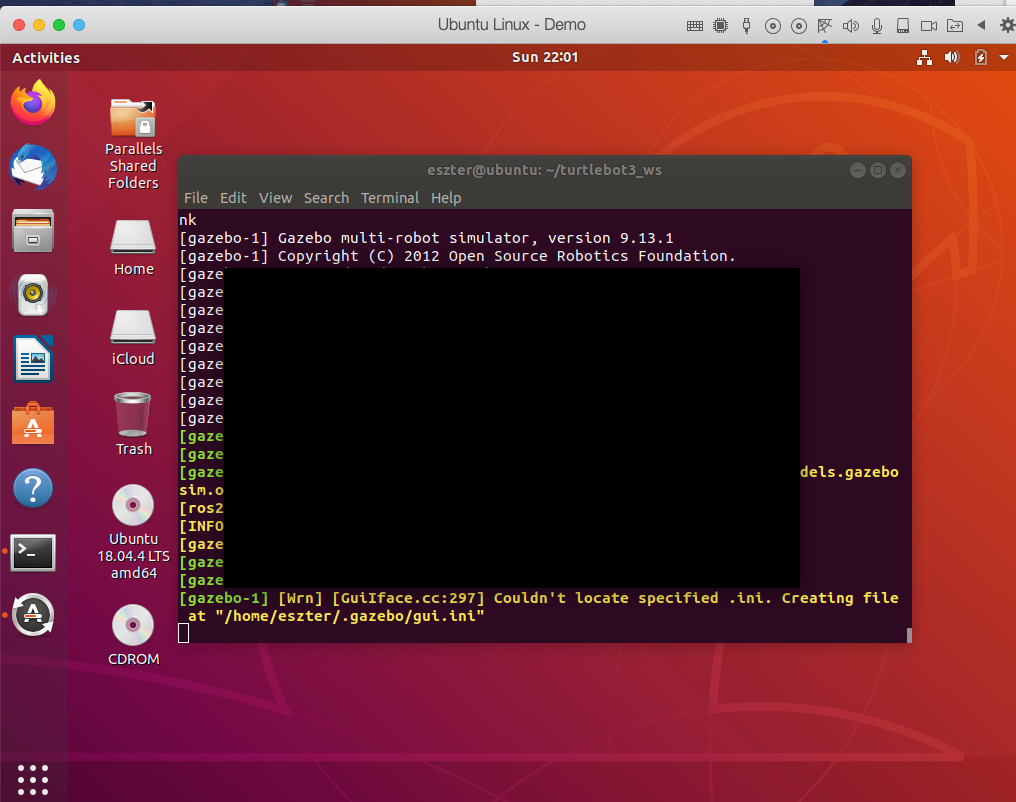
\includegraphics[width=.65\textwidth]{BlackScreen.png}
    \caption{Black Screen at Start of Gazebo}
    \label{fig:blackros2vm}
  \end{center}
\end{figure}
\newline
However, after that you should be able to see the TurtleBot. It is possible to zoom and look at the TurtleBot from different angles and also add more objects to the simulation as seen in figure \ref{fig:gazebo2vm}.\\
\begin{figure}[h!]
  \begin{center}
    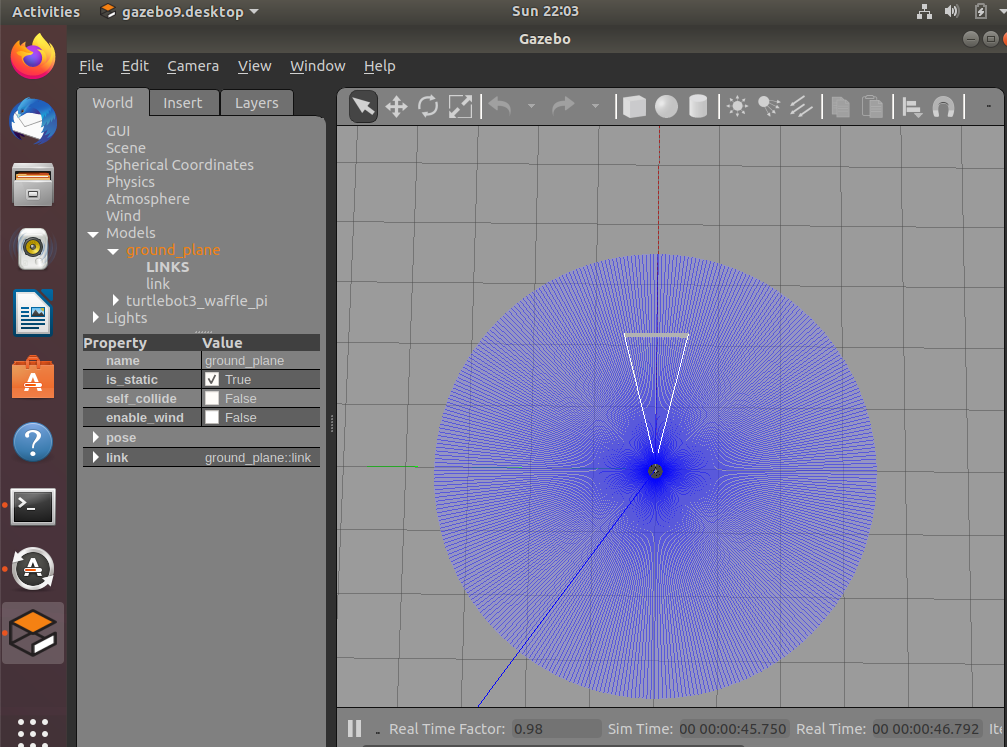
\includegraphics[width=.65\textwidth]{TurtlebotROS2Simulation.png}
    \caption{TurtleBot 3 Simulation}
    \label{fig:gazebo2vm}
  \end{center}
\end{figure}
\newline 
If you want to navigate the TurtleBot with your keyboard, you need to use Teleoperation as seen in section \ref{sec:teleoperation}. 

\newpage
\subsection{VM}
For all installations, a setup of the VM is needed. Any VM on the market can be used. Good experiences have been made with Parallels Desktop (macOS), Virtualbox (Windows, macOS) and VMWare (Windows).
\newline

It should be noted that the \textit{3D / hardware acceleration} setting should be disabled in each virtual machine software since it seems to cause issues when launching instances of the gazebo software. The exact denomination and position of this setting within the respective virtual machine software should be found within the documentation of the used VM application.\\
\newline
To make sure that the Gazebo software really does not use hardware acceleration, the following command should be used to avoid any unexpected crashes.
\begin{Verbatim}[breaklines=true, breakanywhere=true, baselinestretch=1,fontsize=\scriptsize,numbers=left,frame=single,stepnumber=5,xleftmargin=1cm,xrightmargin=1cm]
$ export LIBGL_ALWAYS_SOFTWARE=1
    \end{Verbatim}
    

\subsection{Teleoperation}
\label{sec:teleoperation}
Teleoperation is a command-line tool that can be used to navigate the TurtleBot and arm in the simulation environment \cite{teleop2}. With that, you can navigate the robot with your keyboard. It works the same in ROS1 as in ROS 2. In AWS, it works the same basically but starting it is a little bit different. Therefore, in the AWS section \ref{code:openman}, it is explained once again.
\newline

\textbf{TurtleBot3}\\
\newline
For that, you need to open a new terminal window and use the following commands:
\begin{Verbatim}[breaklines=true, breakanywhere=true, baselinestretch=1,fontsize=\scriptsize,numbers=left,frame=single,stepnumber=5,xleftmargin=1cm,xrightmargin=1cm]
 $ export TURTLEBOT3_MODEL=waffle_pi
 $ ros2 run turtlebot3_teleop teleop_keyboard
    \end{Verbatim}
Again, you can use here also the other Turtlebot models (\texttt{waffle},\texttt{burger}). 
You can now navigate the TurtleBot3 using your keyboard with the keys W (up), A (left), S (down), D (right).

To end both the simulation and the Gazebo, use Ctrl and C in each terminal window.\\
\newline
\textbf{OpenManipulator}\\
\newline
Teleoperation for the OpenManipulator can be launched with the following command \cite{openmanipulatorteleop}:
\begin{Verbatim}[breaklines=true, breakanywhere=true, baselinestretch=1,fontsize=\scriptsize,numbers=left,frame=single,stepnumber=5,xleftmargin=1cm,xrightmargin=1cm]
$ roslaunch open_manipulator_teleop open_manipulator_teleop_keyboard.launch
    \end{Verbatim}

You can control now every single joint (e.g. changing their angles) and also the gripper only with your keyboard. Keep in mind, that for using Teleoperation in the simulation environment for the OpenManipulator, you also have to start its simulation environment (as seen in section \ref{code:openman}).

\newpage 
\subsection{Cloud Solutions}
\subsubsection{AWS}
\label{sec:aws}
The Amazon AWS environment allows various simulations using Gazebo, all of this happening in the cloud with the help of \href{https://aws.amazon.com/de/robomaker/}{RoboMaker} \cite{robomaker}. This enables the developers to work remotely and carry out all their work in the cloud without the need to install anything on their machines or requiring any particular hardware. \\
\newline
AWS features:
\begin{itemize}
    \item Development Environment
    \item Simulation Environment (Gazebo)
    \item Fleet management
\end{itemize}
The latter is not needed for setting up the TurtleBot but it might be helpful for companies who might need to monitor multiple robots.
In this documentation, only the development and simulation environment will be discussed.
The downside of AWS is that it is not free.\\
\newline

\Paragraph{AWS Educate}
As a student, it is possible to use AWS Educate. For non-partner institutions, students will be provided a \$30 credit which can be spent within AWS. It should also be noted that the functionalities within AWS Educate are limited. 
Students get access to a AWS Educate Starter account, which is managed by a third party service - Vocareum.
The usage is limited to a year. Once the year is over or the credits are used up, the overall project cannot be accessed anymore. \\
Another downside of AWS Educate is that, while students are able to create other users, it is not possible to attach a login profile or associate keys, as the access is limited. Therefore, the \$30 credits need to be shared among the students.\\
It also needs to be mentioned, that the AWS Free Tier is not applicable for student accounts. Therefore, the AWS Educate account can only be used to discover basic functionalities of AWS but should not be used for sophisticated development.\\
To register for AWS Educate, students need to register \href{https://www.awseducate.com/login?startURL=\%2Fregistration}{here} \cite{awseducatereg}. For registration, only the name of the student, the year of matriculation and graduation year, name of the institution and university e-mail address is necessary.\\
\newline
\newpage
\Paragraph{Pricing}
For a non-AWS-Educate account, running fees are to be expected. Those will be furthered broken down in the following section. It is assumed that the fleet management is not needed within the project.
\begin{itemize}
    \item \textbf{Development Environment} \\
    The development environment in itself is free. However, fees for using Cloud9, where the development environment runs, apply. 
    The prices depend on the chosen instance. E2C (Elastic Compute Store) is needed. Within E2C, several instances can be chosen. However, the \textbf{E2C micro instances} are free for one year and for a total of 750 hours. However, they only have a small amount of consistent CPU resources and only 613 MB RAM. This might not suffice for the TurtleBot application. 
    In the Robomaker example calculation, a m4LargeInstance is used, which is not included in the free tier. It costs \$0.1 per hour \cite{awsprice}.
    \item \textbf{Storage for the development environment}\\
    The virtual machine incl. TurtleBot and ROS needed 22 GB of storage. It should be considered that files for Ubuntu OS were included as well in the VM. However, it is unclear whether only the storage for the application itself and the installed dependencies is needed, or also for the development environment. AWS could not give a response as they never responded to our e-mail.\\
    For storage, Amazon EBS (Elastic Block Store) is needed. In the free tier, 30GB of storage are included. It should be enough for the TurtleBot application. If the storage is extended, fees of \$0.1 per hour are charged \cite{awsebs}.
    \item \textbf{Simulation}
    The simulation can be used for free for 25 hours for a month. It ends when either the month ends or the 25 hours are used up. After that, the pricing depends on the selected region. The cheapest option is the region US East (N. Virginia) \cite{awsprice}. It costs \$0.40 per hour.
\end{itemize}
As an example, a student group of three people want to use Amazon AWS for a TurtleBot project which runs for 12 weeks. It is assumed that they work in total 12 hours per week on the project and the simulation runs while they are working. They spend a total of 144 hours on the project.
Hence, for the E2C m4Large instance for the development environment they are charged 144*0.1=\$14.4
It is assumed that the 30 GB storage is enough for the project so no additional fees apply, as they are staying within the free tier.
Still, the simulation needs to be paid.
There are two possible scenarios (AWS did not give an answer which scenario would apply in a real life situation):
\begin{itemize}
    \item \textbf{Simulation Free Tier applies to the project}\\
    Per month, they are working 56 hours on the project. Therefore, they will reach the 25 hour limit in the third week of their project. These 25 hours can be deducted from the overall needed hours. Therefore, they still need 119 hours. Therefore, 119*0.4=\$47.6 will be charged for the simulation.
    \item \textbf{Simulation Free Tier applies per person}\\
    In this case, the 56 hours are less than the 75 hours they have. Therefore, they have 8 weeks left that need to be covered. In 8 weeks, they program 8 * 12 = 96 hours. For those 96 hours, 96*0.4=\$38.4 are charged.
\end{itemize}
This example allows four possible scenarios (taking the free tier into consideration):
\begin{itemize}
    \item M4Large instance \& 119 hours simulation needed: \$14.4+\$47.6 = \$62
    \item Micro Instance \& 119 hours simulation needed: \$0+\$47.6 = \$47.6
    \item M4Large instance \& 96 hours simulation needed: \$14.4+\$38.4 = \$52.8
    \item Micro Instance \& 96 hours simulation needed: \$0+\$38.4 = \$38.4
\end{itemize}
Therefore, in this example, the project would cost anywhere from \$38.40 to \$62.
\newline
\newpage
\Paragraph{A short note on AWS Educate Credits}
After using AWS with an Educate account, the credits are not deducted immediately, but only a few days later. This complicates the process of monitoring any used credits. As the AWS Educate account is restricted in its functionalities since it is managed by a third party, it is not possible to view the total session time, which in itself was a much needed piece of information.
Thus, it is not transparent how long one student worked in total or per session on a project, and an overview of how many credits were used during a certain session is unavailable. 
That makes it hard to make any estimations as to how long, the 30 Credits a student gets, will be last for within the AWS simulation environment. \\
\newline
In this project, the amount of available credits were not enough to find a suitable solution for the setup of the OpenManipulator arm. All attempts failed. All required packages specified in the documentation of ROBOTIS were downloaded as well as the launch files were specified as required. However, it seems like in order for the arm to work properly within AWS, the project structure needs to be different.\\
\newline
For instance, in the usual setup, all the needed dependencies usually are cloned into the folder catkin\_ws. In Amazon AWS, this folder does not exist. Instead, AWS uses two different folders, one is robot\_ws and the other one is simulation\_ws. \\
Every dependency for the robot is cloned into robot\_ws and every dependency for the simulation of the robot needs to be in simulation\_ws.\\
The issue with OpenManipulator is that the project is designed in a way that this split of dependencies cannot be done without splitting the designed project structure as some dependencies are needed for both the simulation as well as for the robot.\\
Amazon AWS, however, does not allow duplicates in the whole project structure. Hence, having the files in both folders, would create an error. Probably, it is needed to restructure the whole OpenManipulator project from the developers. Unfortunately, we didn't figure it out within our limited AWS Educational credits budget.\\
\newline

Then we attempted to split the project files but got the errors that the launch files could not be found though, although they were correctly specified and existed in the folder linked by the RoboMakerSettings.json file.\\
As our credits were deducted faster than we initially expected, we decided to ask the developers of the OpenManipulator which files are needed for the simulation, and which correspond to the robot. While they responded, they could not give a satisfying answer stating that that they did have any personal experience RoboMaker on AWS and were therefore unable to aid us further as we already tried their suggestion \cite{robotisforumaws}:
\newline
\begin{displayquote}
Hi,
Unfortunately, we haven't created Turtlebot3 example on AWS so there isn't much information about the platform.

If you are trying to implement the TurtleBot3 with OpenMANIPULATOR-X, you might want to try with the [ROS1] Manipulation section information which use different packages.
Thank you.
\end{displayquote}

\newpage
\Paragraph{Setup of TurtleBot in AWS}
The setup shown uses the TurtleBot sample application in AWS and an AWS Educate Starter account.\\ The distribution used will be ROS-Kinetic (ROS 1).\\
\newline
This steps are similar to the ones in \href{ https://robomakerworkshops.com/workshop/}{this tutorial} but modified for AWS Educate users \cite{workshopaws}.\\
\newline
\textbf{0. Setup a cloudformation stack}\\
\newline
To get started, you need to create a cloudformation stack. To do that, open the \textbf{AWS Management Console}. Type in \textbf{CloudFormation} into the Search field.\\
Press the \textbf{Create Stack} button on the top right corner. Choose \textbf{With new resources (standard)}. 
\begin{enumerate}
    \item \textbf{Create stack}\\
    Choose template is ready and then choose upload a template. Download a template from \href{https://s3.amazonaws.com/assets.robomakerworkshops.com/cfn/bootstrap.cfn.yaml}{this website} and save it as a *.yml file \cite{workshopawsyml}.\\
    Upload then this file.
    \item \textbf{Specify stack details}\\
    Leave everything as it is but fill in the field \textbf{s3BucketName} and \textbf{Stack Name}. You can choose any name you want. 
    \item \textbf{Configure stack options}\\
    Dont change anything here and continue to the next step.
    \item \textbf{Review}\\
    Scrolll down to the bottom, tick the capabilities checkbox and then press the button \textbf{Create stack}.\\
\end{enumerate}
You may now wait some minutes until the creation is finished. When the status changes to \textbf{CREATE\_COMPLETE} navigate to the \textbf{Outputs} tab of your stack and save the values of the keys \textbf{RoboMakerS3Bucket} and \textbf{SimulationRole}.\\
It will look like this:

\begin{Verbatim}[breaklines=true, breakanywhere=true, baselinestretch=1,fontsize=\scriptsize,numbers=left,frame=single,stepnumber=5,xleftmargin=1cm,xrightmargin=1cm]
        RoboMakerS3Bucket: testrobot-us-east-1-rmw-assets
        SimulationRole: arn:aws:iam::664267161887:role/robomaker-simulation-role-us-east-1
    \end{Verbatim}

All your data will be saved in this stack you just created.\\ 
\newline
\textbf{1. Setup the Development Environment}\\
\newline
Open the \textbf{AWS Management Console}. In the search field, search for \textbf{AWS RoboMaker} and open it. Go to the section \textbf{Development Environment} and click on the button \textbf{Create environment}. \\
\newline 
In the next screen, you can configure your environment as seen in figure \ref{fig:devEnvAWS}.
\begin{figure}[h!]
  \begin{center}
    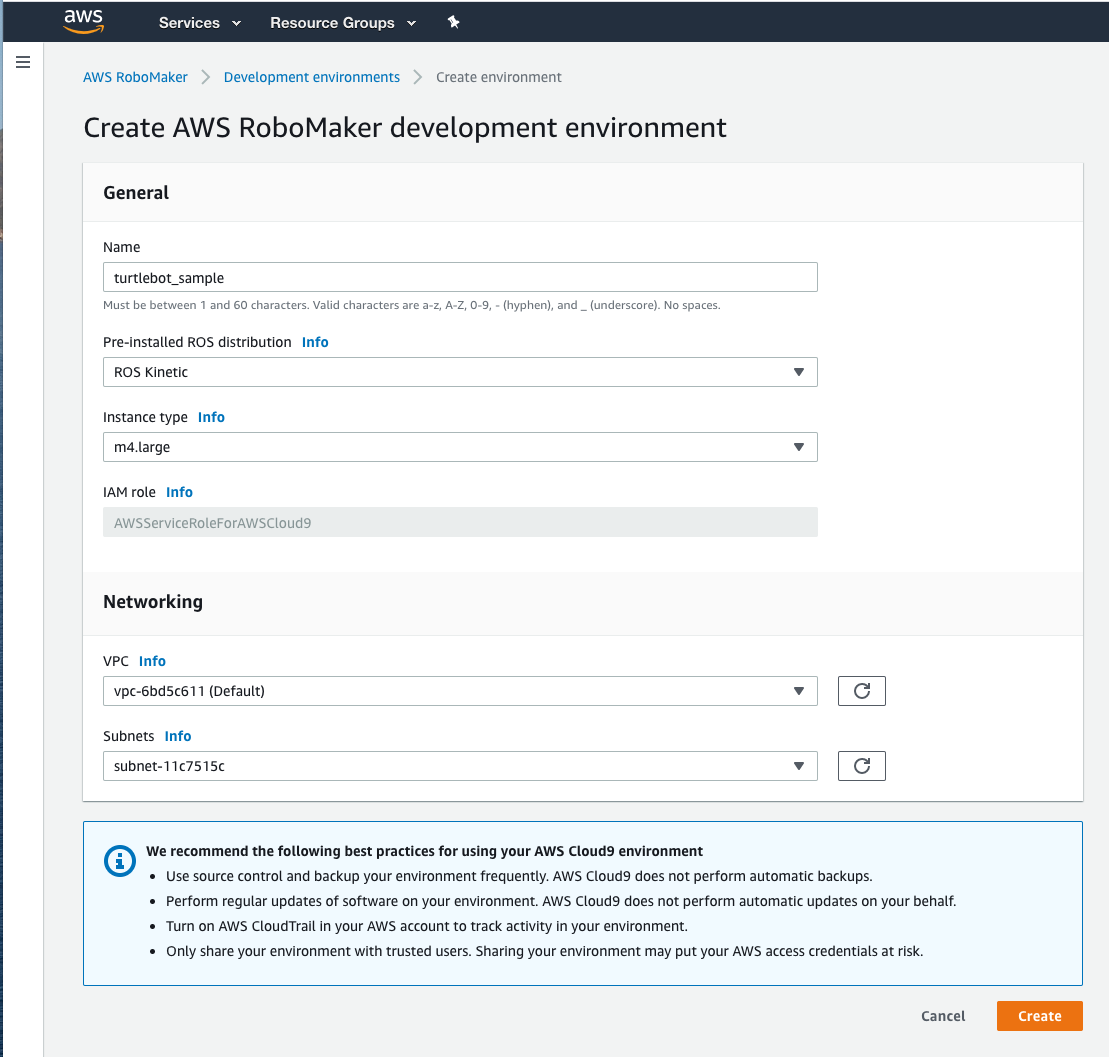
\includegraphics[width=.75\textwidth]{development_environment.png}
    \caption{AWS Development Environment Setup}
    \label{fig:devEnvAWS}
  \end{center}
\end{figure}
In the Name field, the desired name should be entered. The pre-installed ROS-distribution is the one that you want to use for development. In this example, ROS 1 (Kinetic) is used. To use ROS 2, you just need to select ROS Dashing.\\
The instance type is depending on the tasks you want to perform and on your budget. \\
Be aware that \textbf{only the Micro Instance is included in the Free Tier}. 
For Networking choose the Default settings.\\
To continue, press \textbf{Create}.\\
\newline
You might now wait a few minutes until the development environment is setup. Fortunately, the TurtleBot is included in the Sample Application of AWS. Therefore, you can use it as a starting point. To clone the application, press the \textbf{Resources} button, select \textbf{Download samples} and select \textbf{Hello World}. It may take a few minutes as well.\\
\newline
Now, you need to specify the roboMakerSettings.json file. Open it. \\
Search for the s3Bucket property. Once you found it, paste in the value from CloudFormation you created in step 1. Do that for every s3Bucket entry you find in the file.\\
For example:
\begin{Verbatim}[breaklines=true, breakanywhere=true, baselinestretch=1,fontsize=\scriptsize,numbers=left,frame=single,stepnumber=5,xleftmargin=1cm,xrightmargin=1cm]
"simulationApp": {
          "name": "RoboMakerHelloWorldSimulation",
          "s3Bucket": "testrobot-us-east-1-rmw-assets",
    \end{Verbatim}
Next, you need to specify the iamRole. Paste in the value from the key SimulationRole you saved before:
\begin{Verbatim}[breaklines=true, breakanywhere=true, baselinestretch=1,fontsize=\scriptsize,numbers=left,frame=single,stepnumber=5,xleftmargin=1cm,xrightmargin=1cm]
"simulation": {
          "outputLocation": "awsrobomakerhelloworld-159273180411-bundlesbucket-1rvtpu1por607",
          "failureBehavior": "Fail",
          "maxJobDurationInSeconds": 28800,
          "iamRole": "arn:aws:iam::664267161887:role/robomaker-simulation-role-us-east-1"
        }
    \end{Verbatim}
    
\newpage
Lastly, you need to specify your robot model in the launch file. Open the file empty\_world.launch from simulation\_ws -> src -> hello\_world\_simulation -> launch directory.\\
Specify the robot model in the file like this (exchange the Spawn Robot section):
\begin{Verbatim}[breaklines=true, breakanywhere=true, baselinestretch=1,fontsize=\scriptsize,numbers=left,frame=single,stepnumber=5,xleftmargin=1cm,xrightmargin=1cm]

<include file="$(find turtlebot3_description_reduced_mesh)/launch/spawn_turtlebot.launch">
      <arg name="model" value="waffle_pi" />
    </include>
  
\end{Verbatim}
Once this is done, everything is ready for the simulation.
\newline

\textbf{2. Simulating the robot}\\
\newline
To start the simulation, you first need to bundle and build the project. For that, you need to first build the robot. Click on Run -> Build -> HelloWorld Robot and wait until the process is finished.\\
Then click Run -> Build -> HelloWorld Simulation and wait again until it is done.\\
Next, you need to bundle the whole application. For that press Run -> Bundle -> Hello World robot.
The whole process will take up to 15 minutes.\\
\newline
Now, you can go back to your Robomaker console. Go to the \textbf{Simulation Jobs} section. You will see that a process has started. \\
Wait until the status changes to \textbf{Running}. Press then on the simulation job. You should now see a page where you can see details about your job. To view the simulation in Gazebo, scroll down to the \textbf{Simulation application tools} section and press the \textbf{Connect} button in the \textbf{Gazebo} tile. \\
This is also shown in figure \ref{fig:connectGazeboAWS}.
\begin{figure}[h!]
  \begin{center}
    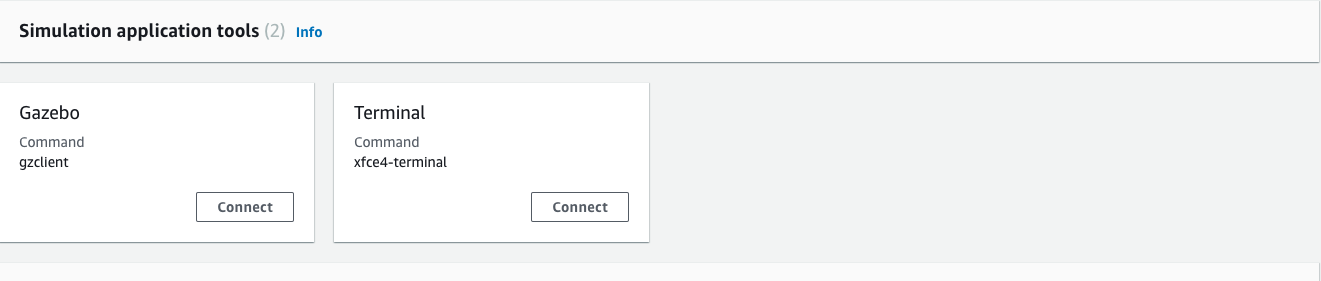
\includegraphics[width=.85\textwidth]{gazebo_connect.png}
    \caption{Connect Gazebo to the Simulation}
    \label{fig:connectGazeboAWS}
  \end{center}
\end{figure}
You should now see your robot running in a new browser window.
\newline

\newpage
\textbf{3. Controlling the TurtleBot}\\
\newline
To start controlling the TurtleBot with Teleop and use the keys of your keyboard, select the simulation job and start Gazebo (as described in the previous step). Leave the window with the simulation open and then select \textbf{Terminal} in the Robot application tools section.
This is also shown in figure \ref{fig:connectTerminalAWS}.\\
\begin{figure}[h!]
  \begin{center}
    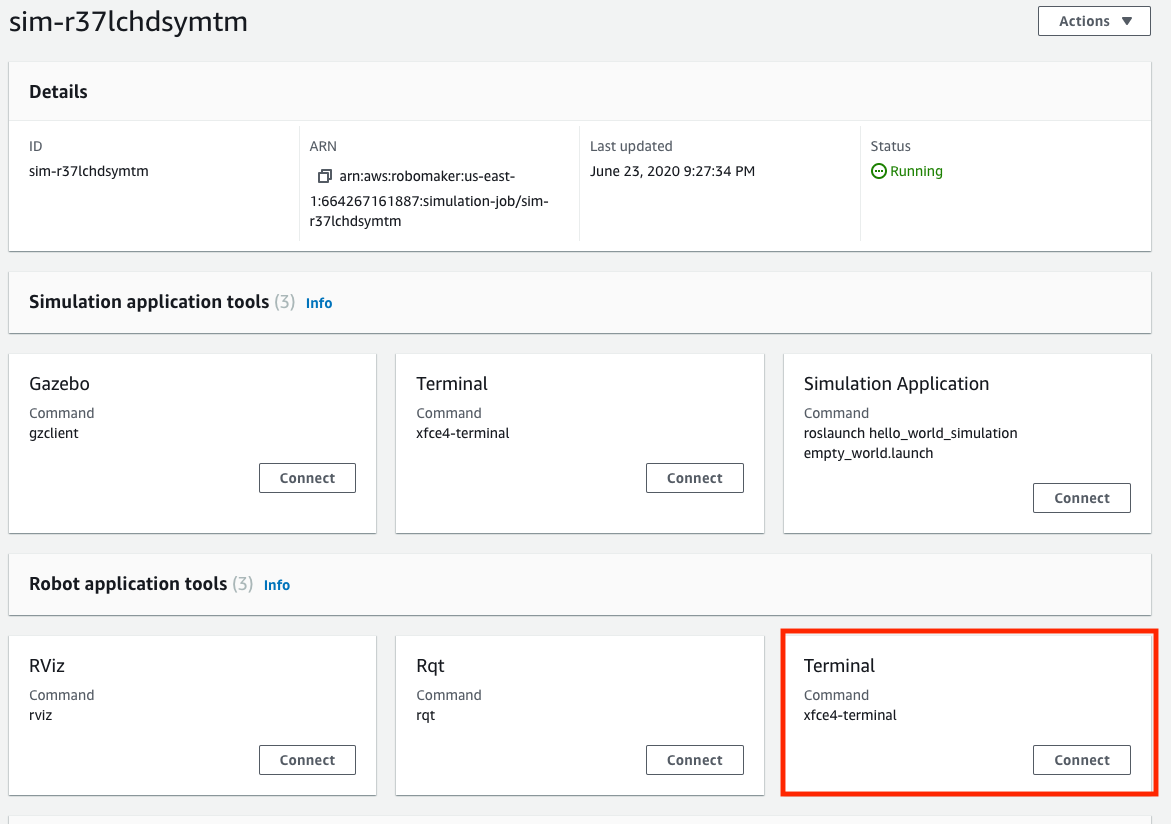
\includegraphics[width=.85\textwidth]{terminal_aws_connect.png}
    \caption{Connect Terminal to simulation}
    \label{fig:connectTerminalAWS}
  \end{center}
\end{figure}

In the upcoming terminal, you can now use \textbf{Teleop} to control the TurtleBot application:\\
\begin{Verbatim}[breaklines=true, breakanywhere=true, baselinestretch=1,fontsize=\scriptsize,numbers=left,frame=single,stepnumber=5,xleftmargin=1cm,xrightmargin=1cm]
$ export TURTLEBOT3_MODEL=waffle_pi
$ roslaunch turtlebot3_navigation turtlebot3_navigation.launch map_file:=$HOME/map.yaml

\end{Verbatim}
You can now control the TurtleBot with your keyboard using the keys A (left), W (up), S (down), D (right). You should be able to see the effect in the Gazebo environment.
\newline

\textbf{4. Stop the simulation}\\
\newline
To stop the simulation, you can either do it from the simulation jobs panel. For that, select your simulation job and press the Cancel button.\\
To stop it from the development environment, open it and choose Simulation -> Stop Simulation\\
\newline
It is very important that you stop your simulation job when it is not needed anymore as costs will apply and credits will be deducted.\\

\newpage
\subsubsection{Gazebo Web}
\label{sec:gazeboweb}
\newline
Gazebo Web is a WebGL client, which provides a Graphical User Interface and visualizations for gazebo simulations in a web browser. For this,2 or more workstations are required. One of the workstations has to set up and run the Gazebo Web server structure consisting of gazebo and NodeJS dependencies. The other workstations can then connect to the server to interact with the simulations.\\
\newline
Due to the Client-Server architecture of the Gazebo Web environment, the only requirement client workstations need to fulfill is having a modern web browser, which supports WebGL and websocket. Therefore the biggest advantage over other simulation options is that the client workstations can be platform-independent, require minimal installation and even support mobile devices. Compared to AWS Cloud, development of the environment and running own code in Gazebo Web is still done locally on the server workstation, but this also means that development and changes can only be done at the centralized server.\\
\newline
Gazebo Web is officially developed by Gazebo, which means constant updates, support for gazebo versions 7 or greater and a large, helpful community.\\ 
\Paragraph{Setup of the Gazebo Web Server}\\
The basis of how to set up gzweb can be found \href{http://gazebosim.org/gzweb.html}{here}. At the bottom of the page you can find further resources to help if you encounter issues in the setup. 
\newline

\textbf{1. Requirements and Dependencies}\\
\newline
All the installation steps focus and need to be implemented on the server. The server workstation first needs to run on ubuntu server version 16.04/18.04 for ROS1/ROS2 respectively. Now after setting up the server, dependencies for gazebo and NodeJS need to be installed. First we install the gazebo packages:\\
\begin{Verbatim}[breaklines=true, breakanywhere=true, baselinestretch=1,fontsize=\scriptsize,numbers=left,frame=single,stepnumber=5,xleftmargin=1cm,xrightmargin=1cm]
$ sudo apt install gazebo7 libgazebo7-dev

\end{Verbatim}
\newline
If you are using ROS2 just substitute the 7 with 9 to get the correct version of gazebo. Now we need to install the rest of the dependencies:\\
\begin{Verbatim}[breaklines=true, breakanywhere=true, baselinestretch=1,fontsize=\scriptsize,numbers=left,frame=single,stepnumber=5,xleftmargin=1cm,xrightmargin=1cm]
$ sudo apt install libjansson-dev nodejs npm nodejs-legacy libboost-dev imagemagick libtinyxml-dev mercurial cmake build-essential

\end{Verbatim}
If they are errors coming up, it is advised to ignore the nodejs-legacy dependency. There might also be conflicts with dependencies of these dependencies. It is therefore recommended to look at the error output and manually install the dependencies that can be seen there.
\newline

\textbf{2. Build Gazebo Web}\\
\newline
To build Gazebo Web Server, we first have to clone the repository and switch to the 1.4.0 release branch:\\
\begin{Verbatim}[breaklines=true, breakanywhere=true, baselinestretch=1,fontsize=\scriptsize,numbers=left,frame=single,stepnumber=5,xleftmargin=1cm,xrightmargin=1cm]
$ cd ~; git clone https://github.com/osrf/gzweb
$ cd ~/gzweb
$ git checkout gzweb_1.4.0

\end{Verbatim}
\newline
In the next steps models and assets (for example the turtlebot wafflepi model), which are used in the simulation have to be gathered and put in the directory "http/client/assets". Furthermore it is important to source the Gazebo setup.sh file:\\
\begin{Verbatim}[breaklines=true, breakanywhere=true, baselinestretch=1,fontsize=\scriptsize,numbers=left,frame=single,stepnumber=5,xleftmargin=1cm,xrightmargin=1cm]
$ source <YOUR_GAZEBO_PATH>/share/gazebo/setup.sh

\end{Verbatim}
\newline
Now it is time to download the specified models from the web:\\
\begin{Verbatim}[breaklines=true, breakanywhere=true, baselinestretch=1,fontsize=\scriptsize,numbers=left,frame=single,stepnumber=5,xleftmargin=1cm,xrightmargin=1cm]
$ npm run deploy --- -m

\end{Verbatim}
To only download local models in the Gazebo model path, simply put local behind the above command. We encountered an error message during the last command, which we could not solve in time, because we only had a single machine, which fulfilled the server requirements and we had to re-purpose it in the end. We did not test the following step therefore.
\newline

\textbf{3. Running the server and connecting clients}\\
\newline
Now that everything is set up, the server can be started by the following command:\\
\begin{Verbatim}[breaklines=true, breakanywhere=true, baselinestretch=1,fontsize=\scriptsize,numbers=left,frame=single,stepnumber=5,xleftmargin=1cm,xrightmargin=1cm]
$ gzserver --verbose

\end{Verbatim}
\newline
The verbose at the end is to see Debug messages. Furthermore gzserver can be also replaced by gazebo. For the next step another terminal has to be opened and following command has to be executed to start the HTTP and Websocket servers:\\
\begin{Verbatim}[breaklines=true, breakanywhere=true, baselinestretch=1,fontsize=\scriptsize,numbers=left,frame=single,stepnumber=5,xleftmargin=1cm,xrightmargin=1cm]
$ npm start

\end{Verbatim}
\newline
Add -p PORTNUMBER to modify the listening port (Default: 8080). The next step is to connect the clients to the server:\\
\begin{Verbatim}[breaklines=true, breakanywhere=true, baselinestretch=1,fontsize=\scriptsize,numbers=left,frame=single,stepnumber=5,xleftmargin=1cm,xrightmargin=1cm]
$ http://localhost:8080

\end{Verbatim}
Here the client is a web browser on the server workstation. To connect a not local client from the network, substitute localhost with the IP address of the server. If the port was modified, substitute the default port with the current one. To stop the server from running, go to the server workstation and press Ctrl+C in the terminals.
\newpage
\section{Comparison of different simulation environments}
\subsection{Usability of different environments}

Some important factors in the decision in which setup environment to use to simulate the TurtleBot 3 are clearly the ease of use and functionality of each simulation environment. Furthermore, the set-up time as well as the compatibility with diverse hardware, should be considered. With that key information in mind, a recommendation as to the optimal workflow can be formulated for future users of the TurtleBot and OpenManipulator arm simulations.

\subsubsection{General Gazebo Simulation Limitations}
Before going through the criteria for every simulation, we would first like to discuss general limitations of gazebo simulation environments in conjuncture with the TurtleBot3 waffle\_pi model and OpenManipulator-X arm, which affects all of the discussed simulation environments. While it was already explained how difficult the set up of these environments can be, this Section focuses more on the usability in these gazebo environments after the installation. The following remarks are a direct result of testing with a laptop, which contains an SSD and an Nvidia graphics card (recommended specifications) running on Ubuntu 16.04 and following the install procedure for section \ref{sec:standalone-ubuntu}.\\ 
\newline
Performance during the testing can be described as inconsistent and unstable at times. The simulation was already lagging sometimes despite adding only minimal objects. Crashes occurred irregularly, especially after leaving the simulation open for a couple of minutes. While crashes are not a problem, because it is very easy to start up the simulation again, the resulting reset of the environment means that all progression is lost, which can be frustrating, especially after spending time positioning the TurtleBot3. This also brings us to the next area: Controlling the TurtleBot3 with Teleoperation and OpenManipulator-X arm with ROBOTIS GUI Controller. Generally the control can be considered clunky. Through Teleop the TurtleBot3 wheel acceleration gets manipulated, making the driving feel more unnatural compared to for example racing simulators. The OpenManipulator-X arm can be manipulated by a graphical user interface, where changes of joint radii are input and send to the arm. The arm then executes the changes in the specified time. When a radius is changed resulting in a collision with another object, the send command gets rejected. This means precise handling is necessary. Because both console for Teleop and GUI for the arm have to be open, the screen becomes convoluted, which can seen in figure \ref{fig:gazsim1}.
\newline
\begin{figure}[h!]
  \begin{center}
    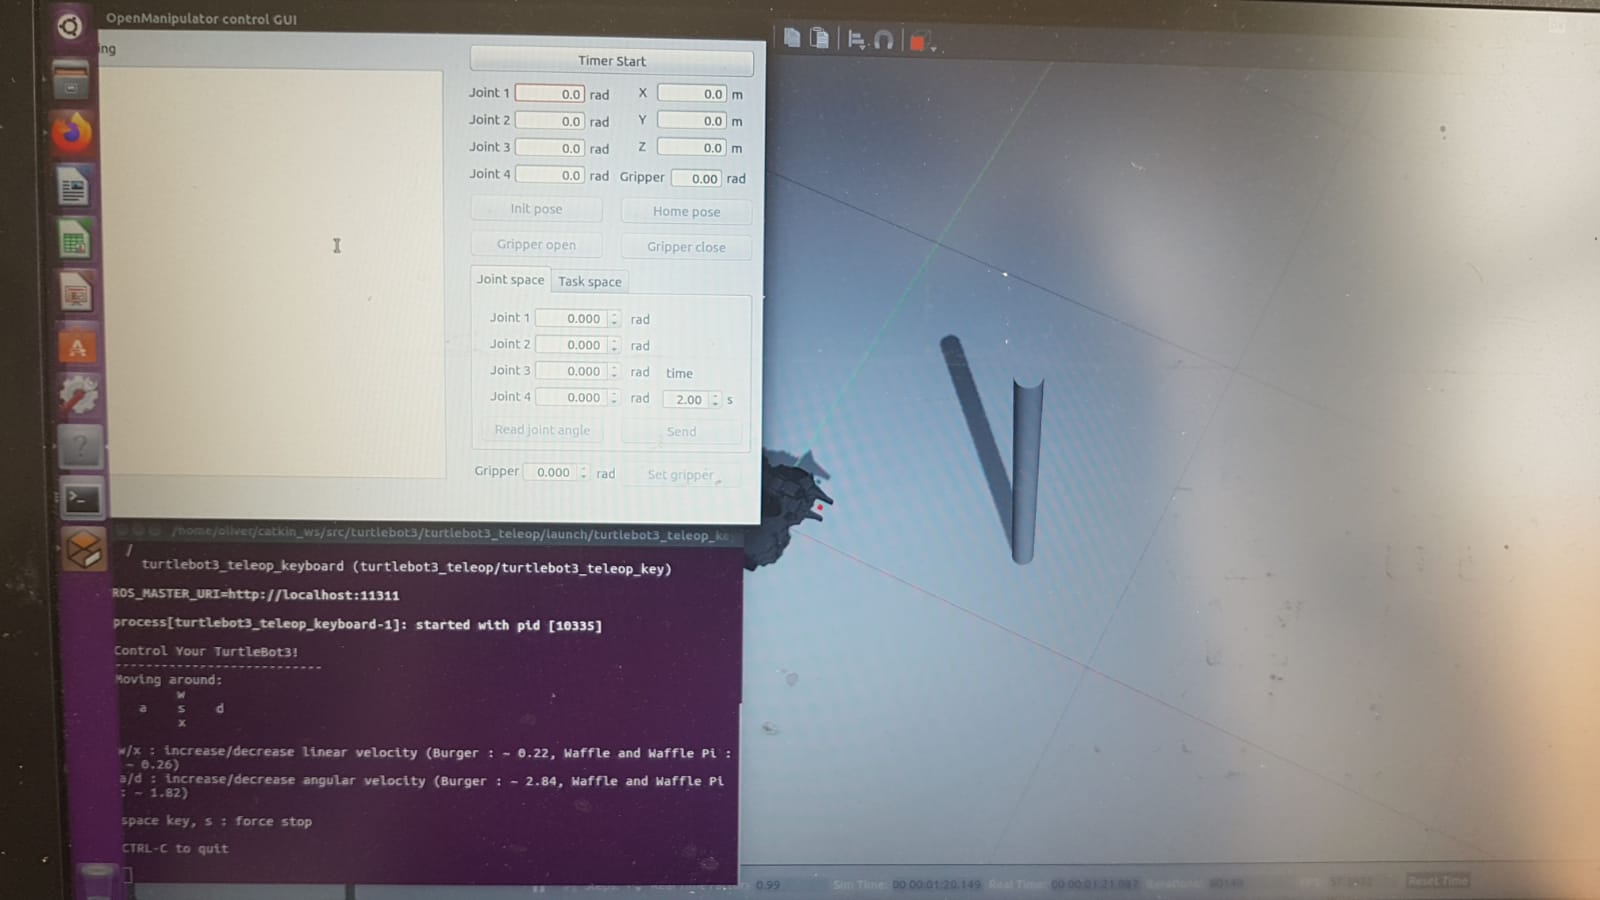
\includegraphics[width=.75\textwidth]{GazeboSim1.jpeg}
    \caption{Simulation Interface with teleop console and arm GUI}
    \label{fig:gazsim1}
  \end{center}
\end{figure}\\
The next area of interest are the objects themselves. The model of the TurtleBot3 waffle\_pi needs to be downloaded from the TurtleBot3 package. This model inhibits incorrect properties making it painful to use. An example of this is a scenario where a smaller object gets grabbed by the arm. If the arm extends far from the waffle\_pi, the waffle\_pi tilts over in that direction. This is not normal behavior, because the physical equivalent is robust and does not tilt as easily. This might be caused by inaccurate physical properties of the arm. Standard models from Gazebo, which includes a ball, cuboid and cylinder can be added, edited and fused to form more complex structures. The model editor for this is easy and intuitive to use. Importing models also works with a little familiarization period. 
\newline
\begin{figure}[h!]
  \begin{center}
    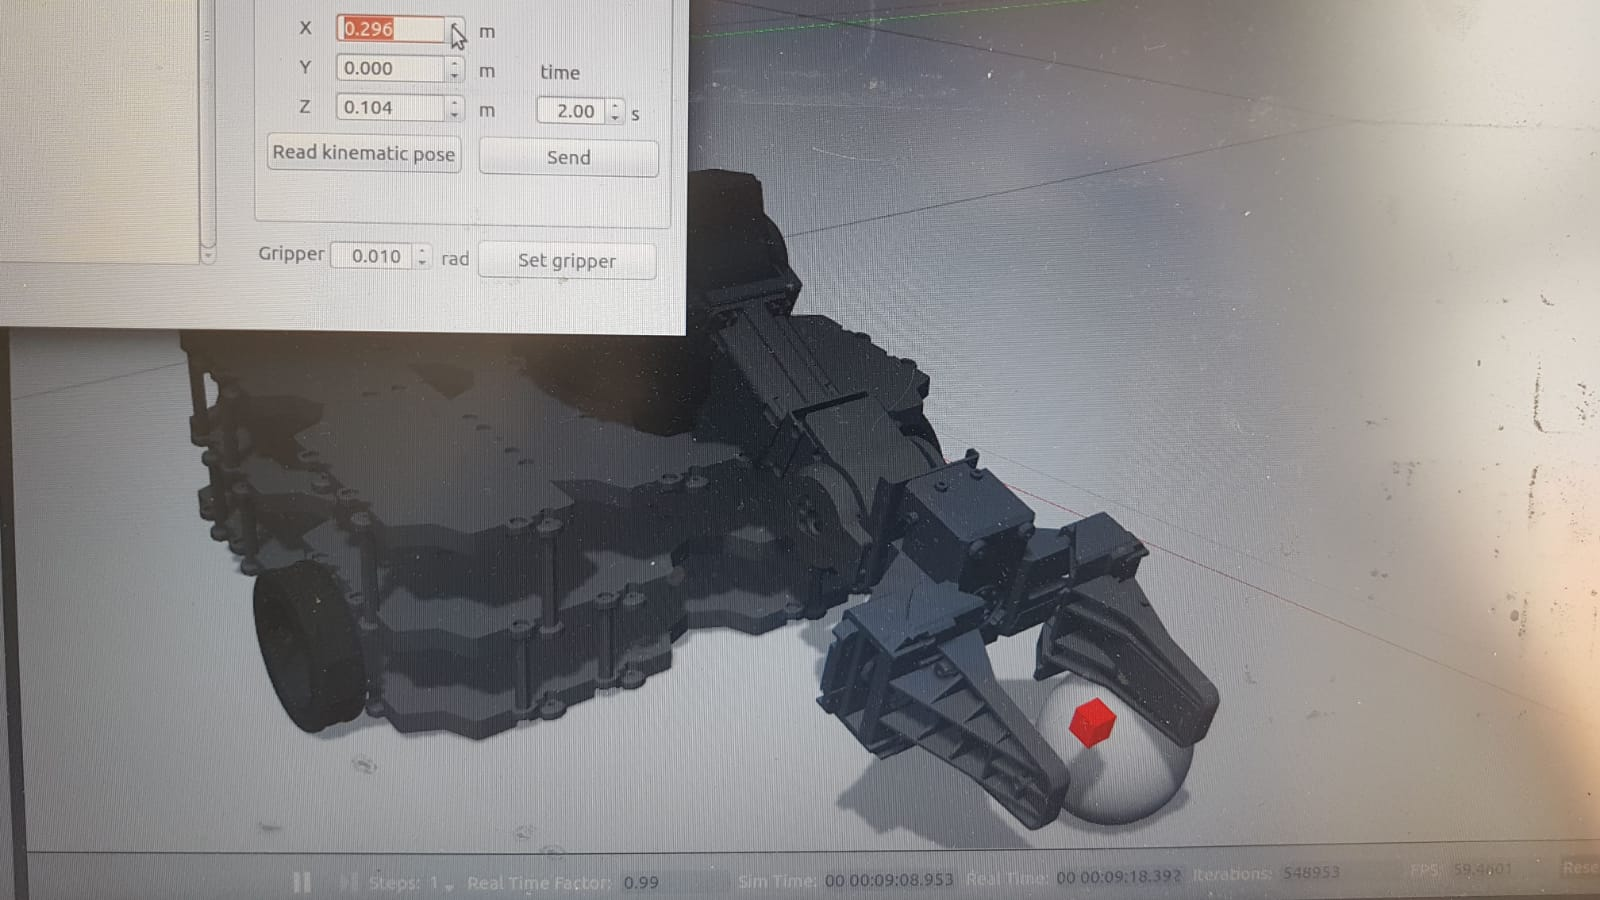
\includegraphics[width=.75\textwidth]{GazeboSim2.jpeg}
    \caption{TurtleBot gets tilted while grabbing a ball}
    \label{fig:gaztilt}
  \end{center}
\end{figure}

\subsubsection{Set-up time}

When it comes to setting up the simulation environments, except when using AWS, it is imperative to download and install the appropriate Ubuntu version. The download should be expected to approximately take around an hour depending on the available internet speed, the install itself averaged at 30 min. 
For the setup of the Open-Manipulator arm as well as the TurtleBot 3 itself, around an hour and thirty minutes were necessary respectively to complete the setups. Those times were the same for both Ubuntu versions and did not differ within the different install environments, such as VMs or standalone installations. This means that the installation of the TurtleBot under ROS 2 amounted to a shorter setup time, since the Open-Manipulator Arm did not have to be installed due to its incompatibly with the OpenManipulator Arm. \\
\newline
However, it should be noted in case of an error during the setup, it is easier to roll back to a previous version of the operating system on a VM than it is a dual boot or a standalone installation. Furthermore, reinstalling Linux in a dual boot can lead to problems with the bootloader setup affecting any other operating systems present on the drive of the Linux installation. This makes the installation process more tedious in dual boot systems, clearly putting VMs at a clear advantage when it comes to reinstallation time, closely followed by the standalone installation. \\
\newline
In AWS, the setup of ROS 1 without the OpenManipulator arm, took half an hour. No times could be recorded for the setup of the OpenManipulator arm since the installation could not be completed due to technical issues. 
Due to unsuccessful setup of Gazebo Web cause by unresolved node dependencies and a failing TurtleBot integration, we are unable to formulate any kind of estimates as to necessary setup time.\\
\newline
This leads to the conclusion that when it comes to the set-up time, AWS clearly is the fastest solution to implement by a clear margin. However, if an implementation of the simulation environment with a functioning OpenManipulator-X needs to be achieved, the best solution is to use a VM with a ROS 1 installation since in case of an error occurring during the installation, less time is lost if a re-installation of the OS is necessary. \\
\newline

\begin{table}[h!]
\centering
\begin{tabular}{l|cc|cc|cc|c|c}
\textbf{Environments} & \multicolumn{2}{c|}{\textbf{VM}} & \multicolumn{2}{c|}{\textbf{Standalone Ubuntu}} & \multicolumn{2}{c|}{\textbf{Dual-Boot}} & \textbf{AWS} & \textbf{Gazebo Web} \\ \hline
\textbf{ROS Version} & \textit{ROS 1} & \textit{ROS 2} & \textit{ROS 1} & \textit{ROS 2} & \textit{ROS 1} & \textit{ROS 2} & \textit{ROS 1} & - \\
\textbf{\begin{tabular}[c]{@{}l@{}}Functioning Open \\ Manipulator Arm\end{tabular}} & yes & no & yes & no & yes & no & no & - \\
\textbf{\begin{tabular}[c]{@{}l@{}}Average total \\ Set-up time (in h)\end{tabular}} & 3:00 & 2:30 & 3:00 & 2:30 & 3:00 & 2:30 & 0:30 & \multicolumn{1}{l}{Failed Set-up}
\end{tabular}
\caption{Set-up times of the TurtleBot Simulation Environments}
\label{tab:setup_times}
\end{table}

\subsubsection{Compatibility with different hardware}

In the available documentation for the TurtleBot 3 simulation environments, no exact minimum hardware requirements are listed. However, throughout the different attempt at setting up the simulation environments, some clear hardware limitations became apparent.\\


\textbf{1. Standalone/Dual Boot}\\
In case of the standalone installations of Ubuntu of course requires a separate drive for the OS, if a dual boot set-up is preferred, the installation drive should be large enough to be able to fit the two operating systems and the TurtleBot and OpenManipulator-X installation. A minimum of 5 GB of hard-drive space should be available. \\
\newline
Regarding graphics, using an integrated graphical unit lead to crashes thus leading to the conclusion that a dedicated graphics card is needed in order to run as intended. 
When using ROS 1, Linux 16.04 is mandatory. However, this might lead to issues with newer AMD graphic cards as no stable drivers are available for older Linux versions. Thus, the system might be unstable. Graphical glitches could be observed as well as crashed at the start-up of the gazebo simulation environment. It is therefore recommended to use a Nvidia graphics card for compatibility. Gazebo seems to generally run more smoothly with a Nvidia GPU than with an AMD, therefore even for ROS 2 a Nvidia GPU is preferred.\\
\newline
As for the processing unit, any relatively modern quadcore should do the trick. No notable difference could be observed between using an AMD or Intel CPU. \\
\newline
Furthermore, the simulation also seems to be very RAM hungry, leading to a recommendation of using at least 8GB to guarantee as smooth workflow.\\

\textbf{2. VM with ROS 1 and ROS 2}\\
When using a VM setup using ROS 1, a dedicated graphical unit is required. A Nvidia GPU is recommended but not required, since the system did run on an AMD GPU, but more stability is guaranteed with a Nvidia graphics card. \\
\newline
For a Virtual Machine running ROS 2, no dedicated GPU is necessary.\\
\newline
As a general rule of thumb, when using a VM installation, a good quad core CPU is needed at least 4 GB of RAM but it is preferred to use 8 GB.\\
\newline
Furthermore, ROS 1 in combination with Ubuntu 16 in a VM on macOS cannot be used. In our tests, Gazebo crashed at the start. The tests were conducted on a 13" MacBook Pro (16 GB RAM, no dedicated graphics card) and on an iMac (32 GB RAM, dedicated AMD graphics card with 8 GB video memory) on macOS Catalina 10.15 using the Parallels VM software. \\
However, ROS 2 in combination with Ubuntu 18 was running fine despite the general known issue, that the OpenManipulator cannot be simulated in ROS 2 and only the TurtleBot3.\\
\newline

\textbf{3. AWS and Gazebo Web}\\
Since both simulation environments use external computational power to run, there are no hardware requirements since only a browser is needed to run the simulation.\\
However, the host PC of Gazebo Web should meet the meet the hardware requirements detailed in the section \ref{sec:standalone-ubuntu}.

\begin{table}[h!]
\resizebox{\textwidth}{!}{
\centering
\begin{tabular}{c|l|ll|ll|c|c}
\multicolumn{1}{l|}{\textbf{Environments}} & \multicolumn{1}{c|}{\textbf{Hardware}} & \multicolumn{2}{c|}{\textbf{Standalone/Dual Boot}} & \multicolumn{2}{c|}{\textbf{VM}} & \textbf{\begin{tabular}[c]{@{}c@{}}AWS \& \\ GzWeb\end{tabular}} & \textbf{\begin{tabular}[c]{@{}c@{}}GezWeb, \\ Host PC\end{tabular}} \\ \hline
\multicolumn{1}{l|}{\textbf{Ros Version}} &  & \textit{ROS 1} & \textit{ROS 2} & \textit{ROS 1} & \textit{ROS 2} &  & - \\ \cline{1-6} \cline{8-8} 
 & CPU & \begin{tabular}[c]{@{}l@{}}Modern \\ quadcore\end{tabular} & \begin{tabular}[c]{@{}l@{}}Modern \\ quadcore\end{tabular} & \begin{tabular}[c]{@{}l@{}}Modern \\ quadcore\end{tabular} & \begin{tabular}[c]{@{}l@{}}Modern \\ quadcore\end{tabular} &  & \multicolumn{1}{l}{\begin{tabular}[c]{@{}l@{}}Modern \\ quadcore\end{tabular}} \\ \cline{2-6} \cline{8-8} 
 & GPU & \begin{tabular}[c]{@{}l@{}}Nvidia \\ GPU\end{tabular} & \begin{tabular}[c]{@{}l@{}}Dedicated \\ graphics\end{tabular} & \begin{tabular}[c]{@{}l@{}}Dedicated \\ graphics\end{tabular} & \begin{tabular}[c]{@{}l@{}}Integrated \\ graphics\end{tabular} &  & \multicolumn{1}{l}{\begin{tabular}[c]{@{}l@{}}Nvidia \\ GPU\end{tabular}} \\ \cline{2-6} \cline{8-8} 
 & RAM & 4 GB & 4 GB & 4 GB & 4 GB &  & \multicolumn{1}{l}{8 GB} \\ \cline{2-6} \cline{8-8} 
\multirow{-4}{*}{\textbf{\begin{tabular}[c]{@{}c@{}}Required\\ minimum\end{tabular}}} & Storage & 5 GB & 5 GB & 5 GB & 5 GB &  & \multicolumn{1}{l}{16 GB} \\ \cline{1-6} \cline{8-8} 
\cellcolor[HTML]{DCD8D8} & \cellcolor[HTML]{DCD8D8}CPU & \multicolumn{1}{c}{\cellcolor[HTML]{DCD8D8}-} & \multicolumn{1}{c|}{\cellcolor[HTML]{DCD8D8}-} & \multicolumn{1}{c}{\cellcolor[HTML]{DCD8D8}-} & \multicolumn{1}{c|}{\cellcolor[HTML]{DCD8D8}-} &  & \cellcolor[HTML]{DCD8D8}- \\ \cline{2-6} \cline{8-8} 
\cellcolor[HTML]{DCD8D8} & \cellcolor[HTML]{DCD8D8}GPU & \multicolumn{1}{c}{\cellcolor[HTML]{DCD8D8}-} & \cellcolor[HTML]{DCD8D8}Nvidia GPU & \cellcolor[HTML]{DCD8D8}Nvidia GPU & \multicolumn{1}{c|}{\cellcolor[HTML]{DCD8D8}-} &  & \cellcolor[HTML]{DCD8D8}- \\ \cline{2-6} \cline{8-8} 
\cellcolor[HTML]{DCD8D8} & \cellcolor[HTML]{DCD8D8}RAM & \cellcolor[HTML]{DCD8D8}8 GB & \cellcolor[HTML]{DCD8D8}8 GB & \cellcolor[HTML]{DCD8D8}8 GB & \cellcolor[HTML]{DCD8D8}8 GB &  & \cellcolor[HTML]{DCD8D8}- \\ \cline{2-6} \cline{8-8} 
\multirow{-4}{*}{\cellcolor[HTML]{DCD8D8}\textbf{\begin{tabular}[c]{@{}c@{}}Recommended\\ minimum\end{tabular}}} & \cellcolor[HTML]{DCD8D8}Storage & \multicolumn{1}{c}{\cellcolor[HTML]{DCD8D8}-} & \multicolumn{1}{c|}{\cellcolor[HTML]{DCD8D8}-} & \multicolumn{1}{c}{\cellcolor[HTML]{DCD8D8}-} & \multicolumn{1}{c|}{\cellcolor[HTML]{DCD8D8}-} & \multirow{-9}{*}{\textit{\begin{tabular}[c]{@{}c@{}}No \\ requirements,\\    only browser \\ needed\end{tabular}}} & \cellcolor[HTML]{DCD8D8}-
\end{tabular}}
\caption{Recommended and required minimum hardware requirements for simulation environments}
\label{tab:simulation_requirements}
\end{table}


\subsubsection{Ease of use}
The ease of use is determined by how well the simulation environment runs but also by how user friendly the experience is. For such a system, the set-up should be easily reproduced without any major problems and should be accessible to a large user base regardless of their hardware, previous experience with simulation environments and financial means.\\

\textbf{1. Standalone/Dual Boot Linux installation}\\
When it comes to the standalone Ubuntu installation, the setup is relatively time consuming as it might be, the set-up is quite simple and not many issues arise during the process. Only a few additional commands are needed to get the simulation to function, which are not detailed in the available resources quoted by the TurtleBot developers but detailed in this paper in the previous set-up sections. \\
\newline
Even on lower hardware, no lagging could be perceived and the system felt responsive, this creates a comfortable environment for programming purposes. However, since dedicated graphical units are required for both ROS 1 and ROS 2, this implementation of a simulation environment is less accessible to the average user.\\
\newline
An advantage of using a standalone Ubuntu installation is the complete control over the file system. However, if some errors are committed in the setup of the simulation environment and the OS has to be reinstalled, it is time consuming and in the case of a dual boot, can even mess up other operating systems on the system.\\

\textbf{2. Virtual Machine}\\
One major advantage of VMs is, in case of an error, how easily the system can be reverted without any damage to other OS or files on the computer. Linux does not even have to be reinstalled within the VM since the state of the virtual machine can simply be reverted to a prior stable state. This simplifies the installation process immensely. Since resources need to be allocated to the Virtual machine such as RAM or processor cores, it also simplifies the process to pinpoint any problems in the simulation which could be linked to hardware limitations.\\
\newline
However, VMs can be prone to lag time if the main operating system uses up too much resources which does affect the workflow. The allocating of resources to the VM can also be quite a finicky process which requires a lot of trial and error.\\

\textbf{3. AWS and Gazebo Web}\\
When it comes to AWS, for now only the TurtleBot 3 can be simulated, the arm is currently not working. However, the setup in itself of the simulation environment is much simpler as first: neither Linux nor ROS do have to be installed, and second in case of an error, the set-up can be easily binned and reattempted. The setup in itself is also quite simple if the steps enumerated in the AWS set-up section above are followed.\\
\newline
The high level of compatibility of AWS should also be complimented. Tools such as the command line, git and testing software make for a highly flexible experience. Due to the online nature of the AWS ecosystem, code can be run from anywhere on pretty much any hardware, as long as an internet connection is available. Running multiple instances of a simulation is also a possibility, increasing productivity.\\
\newline
However, the AWS system in itself is quite complex and the file structure of the system is inaccessible, reducing the user’s incremental control on their project. It should also be noted that with an AWS educate account, a number of functions such as the IAM (Identity \& Access Management, needed for user management) are unavailable, thus further limiting the control over the project. As an example, collaboration is due to the restricted access in IAM hardly possible.\\
\newline
AWS is also a service which requires payment to be fully used. Some free credits are available to students for research purposes, but the time that those credits buy within the AWS environment do not suffice for any deeper usage other than exploring AWS’s basic functionalities.  For any long-term usage of the AWS service, it should be taking into consideration that it is quite expensive.\\
\newline
It should also be noted that currently the OpenManipulator arm cannot be simulated at this point in AWS.\\
\newline
As for Gazebo Web, thus far, the simulation environment could not be made to run correctly due to dependency issues, rendering it unfit for simulation purposes of the TurtleBot3 and its arm. In itself, it is an interesting system, since it circumvents the need of each project participant having the required hardware to run gazebo. It should therefore in theory simplify collaboration within a team. 

\subsection{Recommended Workflow}
\label{recommended_workflow}
In conclusion, the best solution if the arm and the robot have to simulated, the best option is a standalone installation of Ubuntu 16.04 with ROS 1 with a Nvidia GPU and 8GB of RAM. This option offers the most seamless experience and the most functionality. 
If the hardware requirements cannot be met by all the team members, AWS is a good alternative with sufficient funding. Especially with a higher tier account, teamwork is simplified and remote work is facilitated. However, the work should not involve the OpenManipulator Arm since it could not be simulated yet.\\
\newline
The best option still remains to work with the physical robot in order to avoid all the problems that the simulation of the TurtleBot3 and its arm poses.\\
\newline
As a disclaimer, this recommendation is based upon the available software versions up until August 2020, further changes should be taken into account by the user.



\section{Comparison between ROS 1 and ROS 2}

Both the standalone/dual Boot and Linux installation within a VM can use either ROS 1 or ROS 2. This sparks the question as to which ROS should be used to simulate the TurtleBot3 and the OpenManipulator-X.\\
\newline
Since, if the user wants to use ROS 1, Ubuntu 16.06 has to be used, the compatibility with newer hardware such as newer graphics card is not guaranteed. This can lead to potential glitches or hiccups in the user experience. Since this old version of Linux is also not officially supported anymore, the user is vulnerable to possible unpatched issues and no issues with incompatible hardware will be fixed.\\
However, the use of ROS 1 permits the simulation of the OpenManipulator which is not supported by ROS 2 just yet.
ROS 1 is a more a stable and finished version of ROS which targets Python 2. [citation] Due to it being around for a longer, more resources are available to the user as well as help.\\
\newline
Nonetheless, the developers are now concentrating on the newer version of ROS, which means no new functionalities will be implemented, rendering ROS 2 the more future proof option.\\
ROS 2 offers a more polished experience to its users which, due to being installed in Ubuntu 18.06, increases compatibility with different hardware. A few more steps are needed to get it to work than ROS 1, but overall the system runs smoothly on a variety of systems since it is less resource hungry than ROS 1. ROS 2 has been developed to be used with Python 3.5. This implementation is however limited since the OpenManipulator-X cannot be simulated as of yet. 

\begin{table}[h!]
\centering
\begin{tabular}{l|l|l}
 & \textbf{ROS 1} & \textbf{ROS 2} \\ \hline
\textbf{Ubuntu   Version} & 16.04 & 18.04 \\
\textbf{Support TurtleBot   3} & yes & yes \\
\textbf{Support Open   Arm Manipulator} & yes & no \\
\textbf{Python   version} & 2.0 & 3.5 \\
\textbf{Still Supported} & no & yes
\end{tabular}
\caption{ROS 1 vs. ROS 2}
\label{tab:ros1_vs_ros2}
\end{table}

 % Optional
 \section{Further possible simulation environments}
 Several other alternatives are available to simulate the TurtleBot and its arm. Some of them were attempted within the scope of this paper:\\
 \Paragraph{Windows}
 The setup of Windows is described in the TurtleBot documentation  \href{https://emanual.robotis.com/docs/en/platform/turtlebot3/pc_setup/\#windows-setup-remote-pc}{here}.\\
 However, the installation of the required packages and prerequisites such as Visual Studio and the Windows SDK, took quite a long time (2 hours). In the end, the command "catkin\_make", which is the command to build the whole project, failed. After trying it on different machines and also asking on different developer platforms, this issue was confirmed as a bug by the TurtleBot developers. \\
 For some users, updating the Protobuf library solved the issue. \\
 Hence, even developing in a Windows environment is not possible as it won't be possible to build the whole package. While it might be possible to write code on Windows, certainly a second Ubuntu machine will be needed for building it and testing. \\
 
 \Paragraph{Other Cloud environments}
 Another idea is to use different cloud environments such as Axure or Google Cloud. For the latter, educational credits are not available at this moment. For Axure, theoretically, students might be able to get \$ 100 credits. However, the application as a TU Dresden student failed as it sent a message stating that the university TU Dresden is not eligible for credits.\\
 \newline
 It is important to notice that only Amazon AWS offers a dedicated robot development environment. Google and Microsoft's solutions could be used for outsourcing the resource consuming simulation environment Gazebo. The idea behind this technology, is that in the cloud, an Ubuntu server could be used to run Gazebo Web and hence, as a developer, you would not need a dedicated PC to run the Gazebo Web Server. However, generally the same issues as described in section \ref{sec:gazeboweb} are expected.
 \newline
 \Paragraph{Cloud Gaming PCs}
 Also Cloud Gaming PC solutions such as 
 \href{https://shadow.tech/dede}{Shadow} were evaluated and tried. Theoretically, Cloud Gaming PCs offer the benefit to remotely access a computer with powerful hardware, even from a device such as a tablet. Still, there are two issues as to why this solution is not suitable for the TurtleBot environment. First, as described in earlier sections, the setup on Windows is unable to build. The second, is that due to
 \href{https://help.shadow.tech/hc/en-gb/articles/360000455174-Rules-and-Restrictions-on-Shadow#h\_516367ba-b56a-4619-920d-a8223cb588f8}{Shadow's ToC}, the user is banned from setting up a virtual machine.
\newpage
\section{Conclusion}
 This paper started with the motivation to be able to guide any future researchers wishing to use the TurtleBot 3 along with its simulation environment to program it to take up some kind of support role in the elderly care department. Specific simulation environments to analyse were chosen, personas which could be a target of the helping features of TurtleBot3 were conceptualised and some precise Use Cases were formulated with the limitations of the robot in mind. Another goal was to also keep the suggested Use Cases relatively simple in order to be accessible to a wider public of developers.\\
 \newline
 However, along the way it became pretty clear that the numerous limitations of the simulation environment, the robot itself as well as the needed setup needed to be taken into account to be able to express clear guiding steps to aid any future development. Throughout the process, a preferred workflow was able to be formulated as well as a relatively fool proof tutorial to guarantee the success of the simulation. Through the analysis of many different simulation environment as well as the comparison between ROS 1 and ROS2, in the recommended workflow section \ref{recommended_workflow}, the best setup which could be achieved which we recommend, was described; facilitating any future development with the simulation environment of the TurtleBot 3. However, it should be kept in mind that not every possible could be explored due to numerous limitations, meaning that either a better alternative is still out there or that maybe the developers might come up with a better working solution. If the need of a simulation of a simulation environment can be circumvented, this should be attempted by any future TurtleBot 3 users, however this setup was not attempted within the scope of this paper.\\
 \newline
 Through the informal survey (section \ref{sec:appendix}) carried out in the Dresden Uniklinikum Dresden, some guiding ideas could be collected us which aided the refinement of the Use cases described in this paper. The defined of personas in section \ref{sec:personas} should also help distinguish who the designed Use Cases are catered towards, in order that future developers have an idea as to in which environment such use cases could be applied. Through the surveys, we were able to identify that the Use Case of handing out medication would be one of the most accepted and useful one that we could design and also the answers of the nurses helped us redefine the social aspect of the TurtleBot 3 focusing more on its ability to listen to its owner rather than being a communication device within a care facility. The guiding aspect of the robot was also refocused on the constraint of an indoor facility rather than too large of an area due to firstly the needs of elderly patients but also the technical limitations of the TurtleBot. \\
 \newline
 It should, however be considered that the survey did not have a large data pool, nor does it claim to be representative of the general opinion of the care facility personnel. Those Use Cases were conceptualised as purely theoretical constructs for now in the section \ref{sec:descriptionusecases}, and any future researchers should conduct a structured analysis as to the feasibility and overall usefulness of the TurtleBot’s 3 functions.\\
 \newline
 Overall, the paper should provide some helpful guidelines for any future developers but also help them avoid any of the frustrating bugs and problems which can happen while setting up the simulation environment. Also, though the described Use Cases, some good ideas should be able to be translated into a research project within the confines of the Human Computer Interaction guidelines. A satisfying list of recommendations were achieved as well as a good description of the different advantages and disadvantages of the robot, giving a good well-rounded picture of the capabilities of the simulation environment as well as the theatrical capabilities of TurtleBot 3 within the care department as an assistance robot.
 \newpage
\begin{appendices}
\label{sec:appendix}
\Paragraph{Hospital Nursing Staff Survey}

The following surveys were carried out in the Universitäts Klinikum Dresden on two separate days and on two separate services. The 'Urology' as well as the UOC also known as the 'Orthopedic and Trauma Surgery' services were chosen for their heavy percentage of elderly patients which are the prime target of the Use Cases described in this paper for the TurtleBot 3.
The survey were carried out orally in German and the answers were recorded on paper for the reader, the survey will be translated in the appendices below. Please note that some meaning could be lost through the translations. An image of the Robot was shown to the participants to help them imagine how the Robot could operate within the Hospital, furthermore the specifications of the TurtleBot3 and its OpenManipulator Arm were explained and detailed. 
The names of the Nurses were kept anonymous for confidentiality purposes, however the participants were informed of the purpose and use of the collected information. The collected data should not be seen as having a real statistical impact, but should merely serve as an introduction but also a motivation to the Use Cases presented in this paper.
A larger and more diverse pool of participants would be needed to really access the possible reception of the analysed robot.

\section{Original, German}

\subsection{Nurse 1, Urology, 17.08.2020}
\textit{1. Würden Sie einen kleinen 50 cm hoher Hilfsroboter mit einem Greifarm, im Rahmen der Patienten-Pflege, als nützlich empfinden?}\\
\newline
Kleine Roboter sind zwar schön kompakt dennoch in einem Krankenhaus sehr unpraktisch. Schon die Betten der Patienten sind relativ hoch und da würde der nicht dran kommen. Plus so ein kleiner Roboter könnte eine Gefahr für die Patienten darstellen, wenn es übersehen wird. Mit so einer kleinen Größe kann ich mir nicht denken, dass so ein Roboter viel erreichen könnte. Dennoch finde ich die Idee von robotischer Hilfe gar nicht so verkehrt. Es ist ja bekannt, dass wir ein Mangel an Personal haben. Heute sind wir 3 Pflegekräfte für einen ganzen Gang und die Patienten müssen früh gewaschen werden und dann müssen wir noch die Medikamente austeilen. Da wäre eine Unterstützung nicht schlecht aber unsere Arbeit kann schlecht von Robotern übernommen werden da unsere Arbeit sehr vielseitig ist und auch viel mit Vertrauen zu tun hat.\\
\newline
\textit{2. Welche der folgenden Aufgabe würde sie solch einen Roboter zutrauen: Verteilung von Medikamenten, Wegführer, Kommunikationsgerät zwischen Patienten und Pflegepersonal.}\\
\newline
Ich könnte mir sehr gut vorstellen, dass so ein Roboter ein Wegführer sein könnte. Unser Krankenhaus ist sehr verwinkelt und es gibt viele verschieden Gebäude. Dennoch wie schon gesagt sieht der mir ganz klein aus wo ich bedenken hätte, dass der übersehen wird und jemand darauf ausrutscht. Was Medikamenten austeilen angeht, schwierig. Man muss den ethischen Aspekt, wenn der Roboter Fehler macht, wer würde dafür verantwortlich sein? An sich aber da alle Akten der Patienten hier digital festgehalten werde, wäre es eine Möglichkeit, dass ein Roboter diese Aktionen ausführt. Würde uns auf jeden Fall mehr Zeit für andere Aufgaben geben. Als Kommunikationsgerät sehe ich kein Bedürfnis, wir haben da schon eine funktionierende Infrastruktur.\\
\newline
\textit{3. Denken Sie, dass die Patienten so einen Roboter gutheißen würden?}\\
\newline
Bedingt, menschliche Interaktionen sind ein wichtiger Bestandteil der Pflege. Besonders ältere Leute die sonst im Alltag vereinsamen, freuen sich, dass sich unser Personal sie hier pflegt während einer schwierigen Lebensphase. Dennoch kann man nicht die Vorteile übersehen, da uns (das Pflegepersonal) der Roboter Arbeit entnehmen würde, würden wie mehr Zeit für andere Pflegeaufgaben beim Patienten haben, was natürlich für den Patienten mehr und bessere Pflege bedeuten würde. Das kann nur ein Patient erfreuen.
\subsection{Nurse 2, Urology, 17.08.2020}
\textit{1. Würden Sie einen kleinen 50 cm hoher Hilfsroboter mit einem Greifarm, im Rahmen der Patienten-Pflege, als nützlich empfinden?}\\
\newline
Ich bin ein großer Befürwörter der Automatisierung in Krankenhäuser, wir fangen ja langsam alles zu digitalisieren und da ist der nächste natürlicher Schritt Roboter zu benutzen. Einen Greifarm würde sehr hilfreich sein und definitiv dem Roboter fähig machen viel zu machen. 50 cm klingt aber definitiv recht klein, das müsste man sich näher angucken.\\
\newline
\textit{2. Welche der folgenden Aufgabe würde sie solch einen Roboter zutrauen: Verteilung von Medikamenten, Wegführer, Kommunikationsgerät zwischen Patienten und Pflegepersonal.}\\
\newline
Verteilung von Medikamenten kann ich mir sehr gut vorstellen, da würde es natürlich sogar menschliche Fehler vermeiden. Manchmal kann man ja was vertauschen, wenn man Müde, da ist das Risiko geringer mit einer Maschine. Die anderen Funktionen sehe ich jetzt nicht als plausibel. Ein Kommmunikationsgerät brauchen wir nicht wirklich da menschlicher Kontakt in der Pflege immer noch im Vordergrund steht, und wir haben andere Geräte die uns die wichtige Warnung oder Informationen übermitteln. Als Wegweiser ist der Roboter bestimmt nicht geeignet, zu klein denke ich, der würde bestimmt von einen der Bettentransporte überrollt werden. \\
\newline
\textit{3. Denken Sie, dass die Patienten so einen Roboter gutheißen würden?}\\
\newline
Man muss bedenken, dass wir überwiegend ältere Patienten hier auf den Stationen haben, die sind mit Technik jetzt nicht so familiär. Da könnte so ein Roboter sehr befremdlich sein. Auch zu beachten das Pflege auch sehr viel mit menschlichen Gefühlen zu tun hat, da könnte so ein Roboter wirklich nur Routineaufgaben übernehmen, vielleicht nicht unbedingt am Patienten, aber für uns Schwestern als Unterstützung. 
\subsection{Nurse 3, OUC (Orthopedic and Trauma Surgery), 18.08.2020}
\textit{1. Würden Sie einen kleinen 50 cm hoher Hilfsroboter mit einem Greifarm, im Rahmen der Patienten-Pflege, als nützlich empfinden?}\\
\newline
Dieser Roboter sieht echt klein aus, auf der anderen Seite würde es die engen Gänge nicht noch mehr verstopfen. Ob der aber an den Patienten dran kommt ist eine andere Sache. Ein halber Meter ist echt niedrig, an sich ist die Idee eines Hilfsroboter aber schön, wenn es auch gut umgesetzt wird. Da müssten der auch den spezifischen Stationen angepasst werden da die alle verschiedene Bedürfnisse haben.\\
\newline
\textit{2. Welche der folgenden Aufgabe würde sie solch einen Roboter zutrauen: Verteilung von Medikamenten, Wegführer, Kommunikationsgerät zwischen Patienten und Pflegepersonal.}\\
\newline
Ob man eine so wichtige Aufgabe wie die Verteilung von Lebenswichtigen Medikament einem Roboter überlassen kann ist meiner Meinung nach, eine rechtliche Frage für der ich nicht qualifiziert genug bin um die zu beantworten. An sich wäre eine solche Unterstützung natürlich immer willkommen, das würde unser Fachkraft Mangel vielleicht ein bisschen ausgleichen. Als Wegführer könnte der vielleicht im Einsatz kommen innerhalb eines Gebäudes, manchmal ist es recht schwierig manche Stationen zu finden trotz Ausschilderung und manch ältere Patienten haben eh damit einige Probleme. Als Kommunikationsgerät könnte der vielleicht im Einsatz kommen, wenn der Roboter eine Runde drehen würde und sich eine Liste der Bedürfnisse der Patienten machen könnte anstatt, dass wir Schwestern wild von Zimmer zu Zimmer laufen müssen für manchmal recht unwichtige Aufgaben, die wir später erledigen könnten. Das würde vielleicht unser Arbeitsrhytmus verbessern.\\
\newline
\textit{3. Denken Sie, dass die Patienten so einen Roboter gutheißen würden?}\\
\newline
Ich glaube es kommt wirklich darauf an. Im Krankenhaus zu sein kann eine sehr befremdliche Erfahrung sein, und da ist natürlich sehr wichtig, dass wir Schwestern im Kontakt mit unseren Patienten bleiben. Menschlichkeit hat bei uns höchste Priorität und so viel unserer Arbeit könnte uns so ein Roboter nicht abnehmen. Dennoch ist Unterstützung dringend im Pflegebereich gebraucht und da sind Roboter die nächst beste Lösung. Die Zeiten ändern sich und da werden sich die Patienten auch schon daran gewöhnen und vielleicht sogar nur gutheißen. 
\subsection{Nurse 4, OUC (Orthopedic and Trauma Surgery), 18.08.2020}
\textit{1. Würden Sie einen kleinen 50 cm hoher Hilfroboter mit einem Greifarm, im Rahmen der Patienten Pflege, als nützlich empfinden?}\\
\newline
An sich ja, aber wir haben die Erfahrung gemacht das Technik meistens versagt. Das ist dann im Endeffekt keine Untersetzung für den Pflegeteam, sondern eine zusätzliche Belastung. Ich könnte mir aber gut vorstellen, dass das die Zukunft ist. Wir haben ja ein Fachkraftmangel und Roboter sind bestimmt günstiger als Menschenlöhne zu bezahlen. Man muss trotzdem nicht vergessen, dass Pflege ein Beruf ist wo viel Menschlichkeit erfragt ist und ein Verständnis für menschlichen Gefühle, das könnte dieser Roboter zum Beispiel nicht was seine Einsatzbereiche sehr einschränken würde. Ich könnte mir höchstens vorstellen, dass wir den zum Transportieren von Material benutzen können, würde uns natürlich viel Rumrennen sparen.\\
\newline
\textit{2. Welche der folgenden Aufgabe würde sie solch einen Roboter zutrauen: Verteilung von Medikamenten, Wegführer, Kommunikationsgerät zwischen Patienten und Pflegepersonal.}\\
\newline
Die Medikamente müssten wir noch selber vorbereiten, da es eine sehr präzise und wichtige Arbeit sein kann und es ist wichtig, dass dort kein Fehler gemacht wird. Die Verteilung davon könnte aber natürlich ein Roboter machen, das würde uns frühs sehr viel Zeit einsparen, da wir auf Station sehr viele immobile Patienten haben die sehr pflegeintensiv sind. Unter den anderen Funktionen kann ich mir nicht viel Hilfreiches vorstellen, es sind keine Bereiche wo Unterstützung gebraucht wird. Um seinen Weg zu finden gibt es Pläne und sonst werden die Patienten ja eh von unseren Transportkräften zu deren Termine gebracht. \\
\newline
\textit{3. Denken Sie, dass die Patienten so einen Roboter gutheißen würden?}\\
\newline
Es gäbe natürlich eine Gewöhnungszeit da es fremde Technik ist, aber sonst könnte ich mir vorstellen, dass es zum Alltag wird. Manche älteren Patienten könnten damit Probleme haben das sie ja Technik so nicht gewohnt sind aber jüngere Patienten würden sich schnell damit anfreunden. Ganz im Gegenteil, es würde einen modernen Eindruck machen und bestimmt viele Sachen schneller machen was positiv auffallen würde.


\section{Translated, English}
\label{engInterview}
\subsection{Nurse 1, Urology, 17.08.2020}
\textit{1. Do you think that a small Robot with a height of 50cm and a claw arm, could be of any help in the department of patient care?}\\
\newline
Small robots are nice and compact, however in a hospital relatively inconvenient. Already when you consider the height of the patient's bed, they are pretty high and the robot would not reach them. Furthermore, such a small robot could represent a danger to the Patients if they overlook it. I cannot imagine that with such a small height a robot could be capable of achieving many things. However, I find the idea of helping robot quite appealing. It is known that there is a lack of staff. Today we are 3 Nurses for the entire hallway and the patients need to be washed in the morning and then the Medications still have to be handed out. I believe that some support could be welcome but not every aspect of our work can be taken over by robots since our job is very multifaceted and also relies a lot on trust.\\
\newline
\textit{2. Which of the following tasks do you believe such a robot could accomplish: handing out medicine, as a guiding device /path finder, as a communication device between patient and nursing staff.}\\
\newline
I could really well imagine that such a robot could guide patients. Our hospital hallways are vey convoluted and there are many different buildings. But as I already said, the robot looks very small leading me to express the worry that a patient could slip up on it. Regarding handing out medication, it is a difficult point. It is important to consider the ethical questions which arise, if the robot commits a mistake, who would be responsible?
Patient's records are already digitalised; therefore, it would be possible for a robot to carry out such a task. In itself it would definitely give us more time for other tasks. I do not see any use for the communications aspect though, we already have a functioning infrastructure.\\

\newline
\textit{3. Do you believe that such a robot would be welcomed by the patients?}\\
\newline
To a certain extent, human interaction is a very important part of patient care. Especially elderly people who would fall into solitude and are therefore happy to be cared for by our staff during such a difficult time. However, the advantages cannot be ignored, since the robot would alleviate our workload by taking over some tasks, we would have more time to do some specific care tasks, which would mean more care and better care for the patient. This can only have a positive effect on the patient.
\subsection{Nurse 2, Urology, 17.08.2020}
\textit{1. Do you think that a small Robot with a height of 50cm and a claw arm, could be of any help in the department of patient care?}\\
\newline
I am big supporter of automatization within Hospitals, we are slowly starting to digitalise everything and the next natural step if of course to use robots. A claw arm would be very useful and would definitely enable to do many things. However, 50cm does sound quite small, that is something that should be looked more closely at.\\
\newline
\textit{2. Which of the following tasks do you believe such a robot could accomplish: handing out medicine, as a guiding device /path finder, as a communication device between patient and nursing staff.}\\
\newline
I can very well imagine that handing out of medication is a task the robot could take care of, this would even avoid any human error in the process. Sometimes it is possible to mix up medications due to fatigue, this risk is lower with a machine. I do not see the other functions as plausible. Since human interaction is still a very important part of patient care, I do not believe that the robot should be used as a communication device, also we have other equipment which communicated us any vital information or warnings. The robot is certainly not made to be a path finder, it is too small I believer, it would be rolled over by the bed transports. \\

\newline
\textit{3. Do you believe that such a robot would be welcomed by the patients?}\\
\newline
It should be taken into account that predominantly elderly people are here on this service, they are quite unfamiliar with technology. A robot could be a bit disconcerting for them. It should also be considered that a lot of human empathy and feelings are necessary in the care environment, that is why a robot could certainly only take over routine tasks and maybe not necessarily be at the patient’s bed side, but be there as a support for us nurses. 
\subsection{Nurse 3, OUC (Orthopedic and Trauma Surgery), 18.08.2020}
\textit{1. Do you think that a small Robot with a height of 50cm and a claw arm, could be of any help in the department of patient care?}\\
\newline
This robot looks pretty small, on the other hand, it would avoid further clutter in the narrow hallways. Whether the robot will be able to reach patients is another question. Half a meter is a low height, in itself, the idea of a support robot is a nice one if it is implemented correctly. This would also mean that the robot would need to be adjusted to the specific services since we all have different needs.\\
\newline
\textit{2. Which of the following tasks do you believe such a robot could accomplish: handing out medicine, as a guiding device /path finder, as a communication device between patient and nursing staff.}\\
\newline
The question of whether the very important task of distributing medicine should be entrusted to a robot is, in my opinion, a legal one for which I lack the qualification to truly give an answer. In itself such a support is always welcome, especially since it would maybe balance out a bit our staff shortage. The robot could maybe used as a path finder within a building, since it is sometimes a bit difficult to find the right service even with all the directional sign and elderly patients may have orientational problems. The robot could maybe be used as a communication device if it would make a round of the patients in the service and make a list of their needs, instead of us nurses wildly running around from patient to patient to sometimes do some relatively unimportant tasks which we could do at a later point. This could maybe improve our work rhythm. \\
\newline
\textit{3. Do you believe that such a robot would be welcomed by the patients?}\\
\newline
I believe that it really depends. To be at the hospital can be a very disconcerting experience, and because of that it is very important that we Nurses stay in close contact with our patients. Humanity is our highest priority and not that much of our work could be taken over by a robot. However more support in needed in the care department and robots are the next logical solution. Times are changing and patients will get used to it and even welcome the change. 
\subsection{Nurse 4, OUC (Orthopedic and Trauma Surgery), 18.08.2020}
\textit{1. Do you think that a small Robot with a height of 50cm and a claw arm, could be of any help in the department of patient care?}\\
\newline
In itself, yes, however we have made the experience that technology very often breaks down. In this case, technology does not support our nursing team but becomes a hindrance. I could however, very well imagine that this is the future. It is evident that we have a shortage of staff and a robot would certainly be cheaper than paying human wages. It should still not be forgotten that nursing is a job which requires much humanity and an understanding for human emotions, this is something this robot would certainly not be able to do which limits its range of application. At most, I could imagine that it could be used to transport material which would save us a lot of running around.\\
\newline
\textit{2. Which of the following tasks do you believe such a robot could accomplish: handing out medicine, as a guiding device /path finder, as a communication device between patient and nursing staff.}\\
\newline
We would still need to prepare the medicine ourselves since it is a very precise and important work and it is important that no mistake is made. The handing out of the medication could surely be accomplished by the robot, this would save a lot of time in the morning since we have a lot of immobile patients of this service which require a lot specialised care. I do not really know what I should expect from the under the other possible functions, those are not areas in which support is needed. To navigate through the hospital there are maps, and otherwise patients are transported to their appointments by our transportation team.\\
\newline
\textit{3. Do you believe that such a robot would be welcomed by the patients?}\\
\newline
There would naturally be a small familiarization time since it is foreign technology but otherwise I can imagine that it could become part of the day-to-day life. Some elderly patients could have a problem with it since they are not used to newer technologies but younger patients would quickly get used to it. In the contrary, it would make a modern impression and probably speedup a lot of things which would be a positive.
\end{appendices}

\end{document}
